\documentclass[
  final,
  babelLanguage=british,
  desktopVersion,
  %showtrims,
  %overleaf,
]{anecdote-handbook}

%\graphicspath{{./assets/photos/300dpi/}}
\graphicspath{{./assets/photos/92dpi/}}

% Page size: 148mm x 105mm (A6)
%
% Body text: 9.5 / 13.5 pt

\usepackage{local}

%% Details of the book
%% ===================

\title{SBS Monk Training Centre}
\subtitle{Pāli/English Recitations}
\author{SBS Saṅgha}
\publisher{Sāsanārakkha Buddhist Sanctuary}
\date{2021-10-30}% chktex 8
\editionInfo{\textit{First edition}, 2021}
\ISBN{000-0-00000-000-0}

% === Metadata ===

\hypersetup{
  pdftitle={\thetitle},
  pdfauthor={\theauthor},
  pdfcopyright={Copyright (C) 2021, \thePublisher},
  pdfsubject={},% TODO subject
  pdfkeywords={},% TODO keywords
  pdflicenseurl={https://creativecommons.org/licenses/by-nc-nd/4.0/},
  pdfcontacturl={},
  pdflang={en},
}

%% === Load further packages ===

%% === Hyphenation exceptions and corrections ===

\hyphenation{London re-lin-quishes de-ter-mines}

\openany%

\begin{document}

\frontmatter

\ifdesktopversion
\desktopCover{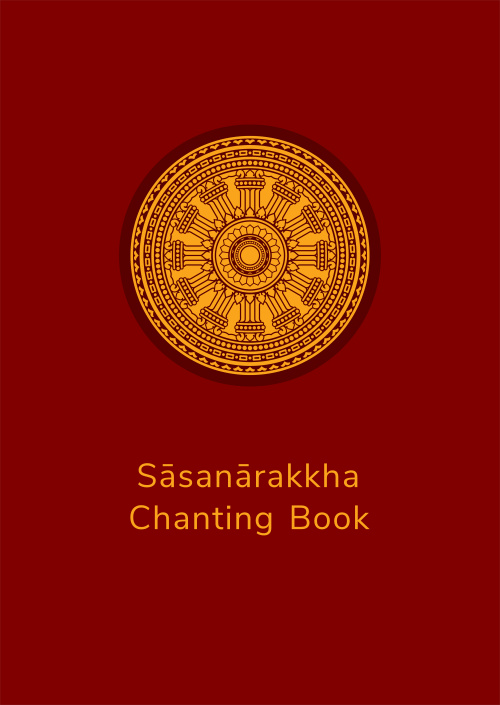
\includegraphics[height=\paperheight]{./handbook-desktop-cover.jpg}}
\fi

\cleartorecto
\thispagestyle{empty}
\vspace*{5em}

{\centering

\settowidth{\titleLength}{%
  {\Large\chapterTitleFont\textls*{\MakeUppercase{\thetitle}}}%
}

{\Large\chapterTitleFont\textls*{\MakeUppercase{\thetitle}}}\\[0.3\baselineskip]
\setlength{\xheight}{\heightof{X}}
\raisebox{0.5\xheight}{\color[gray]{0.4}\rule{\titleLength}{0.25pt}}\\[0.3\baselineskip]
{\itshape \thesubtitle}

\vfill

\vspace*{5em}

}



\cleartoverso
\thispagestyle{empty}

\vspace*{-\baselineskip}

{%

\fontsize{9}{11}\selectfont
\centering
\setlength{\parindent}{0pt}%
\setlength{\parskip}{0.8\baselineskip}%

% \thetitle\\
% \thesubtitle

This book is offered for free distribution,\\
please do not sell this book.

Download this book in PDF, EPUB and MOBI formats\\
at the following address:

\href{https://sasanarakkha.org/}{sasanarakkha.org}

\vfill

Project Manager: Ā. Ariyadhammika\\
Editors: Ā. Devamitta, Ā. Pāladhammika, Ā. Pamodadhammika\\
Typesetting: Ā. Gambhiro, Ā. Pāladhammika\\
Translators: Ā. Aggacitta, Ā. Bodhi, Ā. Sujāto\\
Endnotes: Ā. Ariyadhammika

\vfill

This version was created on:\\
\today\\
\currenttime

\vfill

This work is licensed under a Creative Commons\\
Attribution-NonCommercial-NoDerivatives 4.0 International~License.

Produced with the \LaTeX\ typesetting system,\\
set in Libertinus Serif.

\theEditionInfo

}


% \cleartorecto
\thispagestyle{empty}

{\setlength{\parskip}{10pt}

{\centering\fontsize{20}{25}\selectfont
\textsc{We Wish To Gratefully Acknowledge}
\par}

The Saṅghas of Wat Pah Nanachat (WPN), Amaravati, and Abhayagiri for allowing the use of material from their respective chanting books, the late Ven. Dr. Saddhātissa and Mr. Maurice Walshe for their English translations, as well as Ven. Bhikkhu Bodhi for granting permission to use and slightly adapt his translations. Further contributions are found on the previous page.

\vspace*{1.5\baselineskip}

Additional information on translations, as well as deviations\pagenote{%
  Due to the balanced and inspiring selction of chants, as well as for the sake of
  compatability, the WPN chanting book has served as the basis for the SBS
  chanting book. Over time, suggestions for the inclusion of additional chants, as
  well as occasional improvements of existing translations were incorporated. Such
  changes were meticulously marked down in the endnotes, so that someone familiar
  with the SBS chanting book can straight away find the relevant differences,
  which can be useful when visiting a branch monastery of the Ajahn Chah lineage,
  in order to know in which places to revert to the original version.}
from WPN Chanting Book (2014), have been annotated by Ven. Ariyadhammika in the endnotes.

\bigskip

{\centering
To Āyasmā Aggacitta, the founding father of\\
Sāsanārakkha Buddhist Sanctuary.

\bigskip


\includegraphics[height=65mm]{SBS_logo_Tuck_Loon_BAedit_2020_small.jpg}

}

}


% \chapter{Abbreviations}
\label{abbreviations}

\begin{tabular}{@{}ll@{}}
  \anglebracketleft\ \hspace{-0.5mm}... \hspace{-0.85mm}\anglebracketright\ & \hspace{7.35mm}Only recited by the leader \\
  \hspace{0.1cm} \abbrbreathmark\ & \hspace{7.35mm}Breathing pause \\
\end{tabular}

\begin{tabular}{@{}ll@{}}
  Vin   & Vinaya Piṭaka                                      \\
  DN    & Dīgha Nikāya                                       \\
  MN    & Majjhima Nikāya                                    \\
  SN    & Saṁyutta Nikāya                                    \\
  AN    & Aṅguttara Nikāya                                   \\
  Khp   & Khuddakapāṭha                                      \\
  Dhp   & Dhammapada                                         \\
  Ud    & Udāna                                              \\
  Snp   & Sutta Nipāta                                       \\
  Thag  & Theragāthā                                         \\
  Ja    & Jātaka                                             \\
  % Ps    & Paṭisambhidāmagga                                \\
  Vibh  & Abhidhamma Vibhaṅga                                \\
  Dhs   & Dhammasaṅganī                                      \\
  A     & Aṭṭhakathā (Commentary)                            \\
  MJG   & Mahā-jaya-maṅgala-gāthā (Sri Lanka)                \\
  Thai  & Composed in Thailand, normally in recent centuries \\
  Sri L & Composed in Sri Lanka                              \\
  Trad  & Traditional verses not found in the original Pāli  \\
  WPN  & Wat Pah Nanachat Buddhist Chanting (2014)           \\
\end{tabular}

\bigskip

Wisdom Publication sources: Nikāya and sutta \# (eg. DN 1)\\
P.T.S. sources: Nikāya, volume \#, page \# (eg. D i 1)


\cleartorecto
\pagestyle{toponerow-frontmatter}
\tableofcontents*

\clearpage
\listfirstlines*

\mainmatter
\pagestyle{toponerow}

\cleartorecto
\part{Essential Chants}

{\raggedright

\chapter{Morning Chanting}

\section*{Dedication of Offerings}

[Yo so] bhagavā arahaṃ sammāsambuddho\\
Svākkhāto yena bhagavatā dhammo\\
Supaṭipanno yassa bhagavato sāvakasaṅgho\\
Tam-mayaṃ bhagavantaṃ sadhammaṃ sasaṅghaṃ\\
Imehi sakkārehi yathārahaṃ āropitehi abhipūjayāma\\
Sādhu no bhante bhagavā sucira-parinibbutopi\\
Pacchimā-janatānukampa-mānasā\\
Ime sakkāre duggata-paṇṇākāra-bhūte paṭiggaṇhātu\\
Amhākaṃ dīgharattaṃ hitāya sukhāya\\
Arahaṃ sammāsambuddho bhagavā\\
Buddhaṃ bhagavantaṃ abhivādemi\\\relax
[Svākkhāto] bhagavatā dhammo\\
Dhammaṃ namassāmi\\\relax
[Supaṭipanno] bhagavato sāvakasaṅgho\\
Saṅghaṃ namāmi

\section*{Preliminary Homage}

\begin{leader}
  [Handa mayaṃ buddhassa bhagavato pubbabhāga-namakāraṃ karomase]
\end{leader}

Namo tassa bhagavato arahato sammāsambuddhassa (×3)

\section*{Homage to the Buddha}

\begin{leader}
  [Handa mayaṃ buddhābhitthutiṃ karomase]
\end{leader}

Yo so tathāgato arahaṃ sammāsambuddho\\
Vijjācaraṇa-sampanno sugato lokavidū\\
Anuttaro purisadamma-sārathi\\
Satthā deva-manussānaṃ buddho bhagavā

Yo imaṃ lokaṃ sadevakaṃ samārakaṃ sabrahmakaṃ\\
Sassamaṇa-brāhmaṇiṃ pajaṃ sadeva-manussaṃ sayaṃ abhiññā sacchikatvā pavedesi\\
Yo dhammaṃ desesi ādi-kalyāṇaṃ majjhe-kalyāṇaṃ pariyosāna-kalyāṇaṃ\\
Sātthaṃ sabyañjanaṃ kevala-paripuṇṇaṃ parisuddhaṃ brahma-cariyaṃ pakāsesi\\
Tam-ahaṃ bhagavantaṃ abhipūjayāmi tam-ahaṃ bhagavantaṃ sirasā namāmi

\section*{Homage to the Dhamma}

\begin{leader}
  [Handa mayaṃ dhammābhitthutiṃ karomase]
\end{leader}

Yo so svākkhāto bhagavatā dhammo\\
Sandiṭṭhiko akāliko ehipassiko opanayiko\\
Paccattaṃ veditabbo viññūhi\\
Tam-ahaṃ dhammaṃ abhipūjayāmi tam-ahaṃ dhammaṃ sirasā namāmi

\section*{Homage to the Saṅgha}

\enlargethispage{\baselineskip}

\begin{leader}
  [Handa mayaṃ saṅghābhitthutiṃ karomase]
\end{leader}

Yo so supaṭipanno bhagavato sāvakasaṅgho\\
Ujupaṭipanno bhagavato sāvakasaṅgho\\
Ñāyapaṭipanno bhagavato sāvakasaṅgho\\
Sāmīcipaṭipanno bhagavato sāvakasaṅgho\\
Yadidaṃ cattāri purisayugāni aṭṭha purisapuggalā\\
Esa bhagavato sāvakasaṅgho\\
Āhuneyyo pāhuneyyo dakkhiṇeyyo añjali-karaṇīyo\\
Anuttaraṃ puññakkhettaṃ lokassa\\
Tam-ahaṃ saṅghaṃ abhipūjayāmi tam-ahaṃ saṅghaṃ sirasā namāmi

\section*{Salutation to the Triple Gem}

\begin{leader}
  [Handa mayaṃ ratanattaya-paṇāma-gāthāyo c'eva\\
  saṃvega-parikittana-pāṭhañca bhaṇāmase]
\end{leader}

\firstline{Buddho susuddho karuṇā-mahaṇṇavo}

Buddho susuddho karuṇā-mahaṇṇavo\\
Yo'ccanta-suddhabbara-ñāṇa-locano\\
Lokassa pāpūpakilesa-ghātako\\
Vandāmi buddhaṃ aham-ādarena taṃ\\
Dhammo padīpo viya tassa satthuno\\
Yo magga-pākāmata-bheda-bhinnako\\
Lokuttaro yo ca tad-attha-dīpano\\
Vandāmi dhammaṃ aham-ādarena taṃ\\
Saṅgho sukhettābhyati-khetta-saññito\\
Yo diṭṭha-santo sugatānubodhako\\
Lolappahīno ariyo sumedhaso\\
Vandāmi saṅghaṃ aham-ādarena taṃ\\
Iccevam-ekantabhipūja-neyyakaṃ vatthuttayaṃ \\vandayatābhisaṅkhataṃ\\
Puññaṃ mayā yaṃ mama sabbupaddavā mā hontu ve tassa pabhāva-siddhiyā

Idha tathāgato loke uppanno arahaṃ sammāsambuddho\\
Dhammo ca desito niyyāniko upasamiko parinibbāniko sambodhagāmī sugatappavedito\\
Mayan-taṃ dhammaṃ sutvā evaṃ jānāma

Jātipi dukkhā jarāpi dukkhā maraṇampi dukkhaṃ\\
Soka-parideva-dukkha-domanass'upāyāsāpi dukkhā\\
Appiyehi sampayogo dukkho\\
Piyehi vippayogo dukkho\\
Yamp'icchaṃ na labhati tampi dukkhaṃ\\
Saṅkhittena pañcupādānakkhandhā dukkhā

Seyyathīdaṃ\\
Rūpūpādānakkhandho\\
Vedanūpādānakkhandho\\
Saññūpādānakkhandho\\
Saṅkhārūpādānakkhandho\\
Viññāṇūpādānakkhandho

Yesaṃ pariññāya\\
Dharamāno so bhagavā evaṃ bahulaṃ sāvake vineti\\
Evaṃ bhāgā ca panassa bhagavato sāvakesu anusāsanī bahulā pavattati

Rūpaṃ aniccaṃ vedanā aniccā saññā aniccā saṅkhārā aniccā viññāṇaṃ aniccaṃ

Rūpaṃ anattā vedanā anattā saññā anattā saṅkhārā anattā viññāṇaṃ anattā

Sabbe saṅkhārā aniccā\\
Sabbe dhammā anattā'ti

Te mayaṃ otiṇṇāmha jātiyā jarā-maraṇena\\
Sokehi paridevehi dukkhehi domanassehi upāyāsehi\\
Dukkhotiṇṇā dukkha-paretā\\
Appeva nāmimassa kevalassa dukkha-kkhandhassa\\
antakiriyā paññāyethā'ti

Cira-parinibbutampi taṃ bhagavantaṃ uddissa arahantaṃ sammāsambuddhaṃ\\
Saddhā agārasmā anagāriyaṃ pabbajitā\\
Tasmiṃ bhagavati brahma-cariyaṃ carāma\\
Bhikkhūnaṃ/Sīladharānaṃ sikkhāsājīva-samāpannā\\
Taṃ no brahma-cariyaṃ imassa kevalassa dukkha-kkhandhassa antakiriyāya saṃvattatu

\section*{Closing Homage}

[Arahaṃ] sammāsambuddho bhagavā\\
Buddhaṃ bhagavantaṃ abhivādemi

[Svākkhāto] bhagavatā dhammo\\
Dhammaṃ namassāmi

[Supaṭipanno] bhagavato sāvakasaṅgho\\
Saṅghaṃ namāmi


\input{./manuscript/tex/chants/verses-handbook.tex}
% \chapter{Reflections}

\section{Reflection on the Four Requisites}

\begin{leader}
  [Handa mayaṃ taṅkhaṇika-\\ paccavekkhaṇa-pāṭhaṃ bhaṇāmase]
\end{leader}

\firstline{Paṭisaṅkhā yoniso cīvaraṃ paṭisevāmi}

[Paṭisaṅkhā] yoniso cīvaraṃ paṭisevāmi,\\
yāvadeva sītassa paṭighātāya, uṇhassa paṭighātāya,\\
ḍaṃsa-makasa-vātātapa-siriṃsapa-samphassānaṃ\\
paṭighātāya, yāvadeva hirikopina-paṭicchādanatthaṃ

\begin{english}
  Wisely reflecting, I use the robe: only to ward off cold, to ward off heat, to
  ward off the touch of flies, mosquitoes, wind, burning and creeping things,
  only for the sake of modesty.
\end{english}

[Paṭisaṅkhā] yoniso piṇḍapātaṃ paṭisevāmi, neva davāya, na madāya, na maṇḍanāya,
na vibhūsanāya, yāvadeva imassa kāyassa ṭhitiyā, yāpanāya, vihiṃsūparatiyā,
brahmacariyānuggahāya, iti purāṇañca vedanaṃ paṭihaṅkhāmi, navañca vedanaṃ na
uppādessāmi, yātrā ca me bhavissati anavajjatā ca phāsuvihāro cā'ti

\begin{english}
  Wisely reflecting, I use almsfood: not for fun, not for pleasure, not for
  fattening, not for beautification, only for the maintenance and nourishment of
  this body, for keeping it healthy, for helping with the Holy Life; thinking
  thus, `I~will allay hunger without overeating, so that I may continue to live
  blamelessly and at ease.'
\end{english}

[Paṭisaṅkhā] yoniso senāsanaṃ paṭisevāmi,\\
yāvadeva sītassa paṭighātāya, uṇhassa paṭighātāya,\\
ḍaṃsa-makasa-vātātapa-siriṃsapa-samphassānaṃ\\
paṭighātāya, yāvadeva utuparissaya vinodanaṃ paṭisallānārāmatthaṃ

\begin{english}
  Wisely reflecting, I use the lodging: only to ward off cold, to ward off heat,
  to ward off the touch of flies, mosquitoes, wind, burning and creeping things,
  only to remove the danger from weather, and for living in seclusion.
\end{english}

[Paṭisaṅkhā] yoniso gilāna-paccaya-bhesajja-parikkhāraṃ paṭisevāmi, yāvadeva
uppannānaṃ veyyābādhikānaṃ vedanānaṃ paṭighātāya, abyāpajjha-paramatāyā'ti

\begin{english}
  Wisely reflecting, I use supports for the sick and medicinal requisites: only
  to ward off painful feelings that have arisen, for the maximum freedom from
  disease.
\end{english}

\suttaRef{M.I.10}

\section{Five Subjects for Frequent Recollection}

\begin{leader}
  [Handa mayaṃ abhiṇha-paccavekkhaṇa-pāṭhaṃ bhaṇāmase]
\end{leader}

\firstline{Jarā-dhammomhi jaraṃ anatīto}

\instr{(Men Chant)}

[Jarā-dhammomhi] jaraṃ anatīto

\begin{english}
  I am of the nature to age, I have not gone beyond ageing.
\end{english}

Byādhi-dhammomhi byādhiṃ anatīto

\begin{english}
  I am of the nature to sicken, I have not gone beyond sickness.
\end{english}

Maraṇa-dhammomhi maraṇaṃ anatīto

\begin{english}
  I am of the nature to die, I have not gone beyond dying.
\end{english}

Sabbehi me piyehi manāpehi nānābhāvo vinābhāvo

\begin{english}
  All that is mine, beloved and pleasing,\\
  will become otherwise, will become separated from me.
\end{english}

Kammassakomhi kammadāyādo kammayoni kammabandhu kammapaṭisaraṇo\\
Yaṃ kammaṃ karissāmi, kalyāṇaṃ vā pāpakaṃ vā, tassa dāyādo bhavissāmi

\begin{english}
  I am the owner of my kamma, heir to my kamma, born of my kamma, related to my
  kamma, abide supported by my kamma. Whatever kamma I shall do, for good or for
  ill, of that I will be the heir.
\end{english}

Evaṃ amhehi abhiṇhaṃ paccavekkhitabbaṃ

\begin{english}
  Thus we should frequently recollect.
\end{english}

\instr{(Women Chant)}

[Jarā-dhammāmhi] jaraṃ anatītā

\begin{english}
  I am of the nature to age, I have not gone beyond ageing.
\end{english}

Byādhi-dhammāmhi byādhiṃ anatītā

\begin{english}
  I am of the nature to sicken, I have not gone beyond sickness.
\end{english}

Maraṇa-dhammāmhi maraṇaṃ anatītā

\begin{english}
  I am of the nature to die, I have not gone beyond dying.
\end{english}

Sabbehi me piyehi manāpehi nānābhāvo vinābhāvo

\begin{english}
  All that is mine, beloved and pleasing,\\
  will become otherwise, will become separated from me.
\end{english}

Kammassakāmhi kammadāyādā kammayoni kammabandhu kammapaṭisaraṇā\\
Yaṃ kammaṃ karissāmi, kalyāṇaṃ vā pāpakaṃ vā, tassa dāyādā bhavissāmi

\begin{english}
  I am the owner of my kamma, heir to my kamma, born of my kamma, related to my
  kamma, abide supported by my kamma. Whatever kamma I shall do, for good or for
  ill, of that I will be the heir.
\end{english}

Evaṃ amhehi abhiṇhaṃ paccavekkhitabbaṃ

\begin{english}
  Thus we should frequently recollect.\\
  \suttaRef{A.III.71}
\end{english}

\section{Ten Subjects for Frequent Recollection}

\firstline{Dasa ime bhikkhave}

\begin{leader}
  [Handa mayaṃ pabbajita\hyp{}abhiṇha-\\ paccavekkhaṇa\hyp{}pāṭhaṃ bhaṇāmase]
\end{leader}

[Dasa ime bhikkhave] dhammā pabbajitena abhiṇhaṃ paccavekkhitabbā, katame dasa

\begin{english}
  Bhikkhus, there are ten dhammas which should be reflected upon, again and again, by one who has gone forth. What are these ten?
\end{english}

Vevaṇṇiyamhi ajjhūpagato'ti pabbajitena abhiṇhaṃ paccavekkhitabbaṃ

\begin{english}
  `I am no longer living according to worldly aims and values.'\\
  This should be reflected upon, again and again,\\
  by one who has gone forth.
\end{english}

Parapaṭibaddhā me jīvikā'ti pabbajitena abhiṇhaṃ paccavekkhitabbaṃ

\begin{english}
  `My very life is sustained through the gifts of others.'\\
  This should be reflected upon, again and again,\\
  by one who has gone forth.
\end{english}

Añño me ākappo karaṇīyo'ti pabbajitena abhiṇhaṃ paccavekkhitabbaṃ

\begin{english}
  `I should strive to abandon my former habits.'\\
  This should be reflected upon, again and again,\\
  by one who has gone forth.
\end{english}

Kacci nu kho me attā sīlato na upavadatī'ti pabbajitena abhiṇhaṃ paccavekkhitabbaṃ

\begin{english}
  `Does regret over my conduct arise in my mind?'\\
  This should be reflected upon, again and again,\\
  by one who has gone forth.
\end{english}

Kacci nu kho maṃ anuvicca viññū sabrahmacārī sīlato na upavadantī'ti pabbajitena abhiṇhaṃ paccavekkhitabbaṃ

\begin{english}
  `Could my spiritual companions find fault with my conduct?'\\
  This should be reflected upon, again and again,\\
  by one who has gone forth.
\end{english}

Sabbehi me piyehi manāpehi nānābhāvo vinābhāvo'ti pabbajitena abhiṇhaṃ paccavekkhitabbaṃ

\begin{english}
  `All that is mine, beloved and pleasing, will become otherwise, will become separated from me.'\\
  This should be reflected upon, again and again,\\
  by one who has gone forth.
\end{english}

Kammassakomhi kammadāyādo kammayoni kammabandhu kammapaṭisaraṇo, yaṃ kammaṃ karissāmi, kalyāṇaṃ vā pāpakaṃ vā, tassa dāyādo bhavissāmī'ti pabbajitena abhiṇhaṃ paccavekkhitabbaṃ

\begin{english}
  `I am the owner of my kamma, heir to my kamma,\\
  born of my kamma, related to my kamma,\\
  abide supported by my kamma; whatever kamma I shall do,\\
  for good or for ill, of that I will be the heir.'\\
  This should be reflected upon, again and again,\\
  by one who has gone forth.
\end{english}

`Kathambhūtassa me rattindivā vītipatantī'ti pabbajitena abhiṇhaṃ paccavekkhitabbaṃ

\begin{english}
  `The days and nights are relentlessly passing; how well am I spending my time?'\\
  This should be reflected upon, again and again,\\
  by one who has gone forth.
\end{english}

Kacci nu kho'haṃ suññāgāre abhiramāmī'ti pabbajitena abhiṇhaṃ paccavekkhitabbaṃ

\begin{english}
  `Do I delight in solitude or not?'\\
  This should be reflected upon, again and again,\\
  by one who has gone forth.
\end{english}

Atthi nu kho me uttari-manussa-dhammā alamariya-ñāṇa-dassana-viseso adhigato, so'haṃ pacchime kāle sabrahmacārīhi puṭṭho na maṅku bhavissāmī'ti pabbajitena abhiṇhaṃ paccavekkhitabbaṃ

\begin{english}
  `Has my practice borne fruit with freedom or insight so that at the end of my life I need not feel ashamed when questioned by my spiritual companions?'\\
  This should be reflected upon, again and again,\\
  by one who has gone forth.
\end{english}

Ime kho bhikkhave dasa dhammā pabbajitena abhiṇhaṃ paccavekkhitabbā'ti

\begin{english}
  Bhikkhus, these are the ten dhammas to be reflected upon, again and again, by one who has gone forth.
\end{english}

\suttaRef{A.V.87}

\section{Caturappamaññā-obhāsana}

\firstline{Mettā-sahagatena}

\begin{leader}
  [Handa mayaṃ caturappamaññā-obhāsanaṃ karomase]
\end{leader}

[Mettā-sahagatena] cetasā ekaṃ disaṃ pharitvā viharati\\
Tathā dutiyaṃ tathā tatiyaṃ tathā catutthaṃ\\
Iti uddhamadho tiriyaṃ sabbadhi sabbattatāya\\
Sabbāvantaṃ lokaṃ mettā-sahagatena cetasā\\
Vipulena mahaggatena appamāṇena averena\\
abyāpajjhena pharitvā viharati

Karuṇā-sahagatena cetasā ekaṃ disaṃ pharitvā viharati\\
Tathā dutiyaṃ tathā tatiyaṃ tathā catutthaṃ\\
Iti uddhamadho tiriyaṃ sabbadhi sabbattatāya\\
Sabbāvantaṃ lokaṃ karuṇā-sahagatena cetasā\\
Vipulena mahaggatena appamāṇena averena\\
abyāpajjhena pharitvā viharati

Muditā-sahagatena cetasā ekaṃ disaṃ pharitvā viharati\\
Tathā dutiyaṃ tathā tatiyaṃ tathā catutthaṃ\\
Iti uddhamadho tiriyaṃ sabbadhi sabbattatāya\\
Sabbāvantaṃ lokaṃ muditā-sahagatena cetasā\\
Vipulena mahaggatena appamāṇena averena\\
abyāpajjhena pharitvā viharati

\clearpage

Upekkhā-sahagatena cetasā ekaṃ disaṃ pharitvā viharati\\
Tathā dutiyaṃ tathā tatiyaṃ tathā catutthaṃ\\
Iti uddhamadho tiriyaṃ sabbadhi sabbattatāya\\
Sabbāvantaṃ lokaṃ upekkhā-sahagatena cetasā\\
Vipulena mahaggatena appamāṇena averena\\
abyāpajjhena pharitvā viharatī'ti \suttaRef{D.I.251}

\subsubsection{Suffusion With the Divine Abidings}

\firstline{I will abide}

\smallskip

\begin{leader}
  [Now let us make the Four Boundless Qualities\\ shine forth.]
\end{leader}

[I will abide] pervading one quarter\\
with a heart imbued with loving-kindness;\\
Likewise the second, likewise the third,\\ likewise the fourth;\\
So above and below, around and everywhere;\\ and to all as to myself.\\
I will abide pervading the all-encompassing\\
world with a heart imbued with loving-kindness;\\
abundant, exalted, immeasurable, without hostility,\\
and without ill-will.

I will abide pervading one quarter\\
with a heart imbued with compassion;\\
Likewise the second, likewise the third,\\ likewise the fourth;\\
So above and below, around and everywhere;\\ and to all as to myself.\\
I will abide pervading the all-encompassing\\
world with a heart imbued with compassion;\\
abundant, exalted, immeasurable, without hostility,\\
and without ill-will.

I will abide pervading one quarter\\
with a heart imbued with gladness;\\
Likewise the second, likewise the third,\\ likewise the fourth;\\
So above and below, around and everywhere;\\ and to all as to myself.\\
I will abide pervading the all-encompassing\\
world with a heart imbued with gladness;\\
abundant, exalted, immeasurable, without hostility,\\
and without ill-will.

I will abide pervading one quarter\\
with a heart imbued with equanimity;\\
Likewise the second, likewise the third,\\ likewise the fourth;\\
So above and below, around and everywhere;\\ and to all as to myself.\\
I will abide pervading the all-encompassing\\
world with a heart imbued with equanimity;\\
abundant, exalted, immeasurable, without hostility,\\
and without ill-will.

\section{Recollection After Using the Requisites}
\label{recollection-after-using}

\begin{leader}
  [Handa mayaṃ atīta-paccavekkhaṇa-pāṭhaṃ bhaṇāmase]
\end{leader}

\firstline{Ajja mayā apaccavekkhitvā yaṃ cīvaraṃ}

Ajja mayā apaccavekkhitvā yaṃ cīvaraṃ paribhuttaṃ, taṃ yāvadeva sītassa
paṭighātāya, uṇhassa paṭighātāya, ḍaṃsa-makasa-vātātapa-siriṃsapa-samphassānaṃ
paṭighātāya, yāvadeva hirikopina paṭicchādan'atthaṃ.

\begin{english}
  Whatever robe I used today without consideration, was only to ward off cold,
  to ward off heat, to ward off the touch of flies, mosquitoes, wind, burning
  and creeping things, only for the sake of modesty.
\end{english}

Ajja mayā apaccavekkhitvā yo piṇḍapāto paribhutto, so n'eva davāya, na madāya,
na maṇḍanāya, na vibhūsanāya, yāvad-eva imassa kāyassa ṭhitiyā, yāpanāya,
vihiṃsūparatiyā, brahmacariyānuggahāya, iti purāṇañca vedanaṃ paṭihaṅkhāmi,
navañca vedanaṃ na uppādessāmi, yātrā ca me bhavissati anavajjatā ca phāsuvihāro
cā'ti.

\begin{english}
  Whatever alms-food I used today without consideration, was not for fun, not
  for pleasure, not for fattening, not for beautification, only for the
  maintenance and nourishment of this body, for keeping it healthy, for helping
  with the Holy Life; thinking thus, `I will allay hunger without overeating, so
  that I may continue to live blamelessly and at ease.'
\end{english}

Ajja mayā apaccavekkhitvā yaṃ senāsanaṃ paribhuttaṃ, taṃ yāvadeva sītassa
paṭighātāya, uṇhassa paṭighātāya, ḍaṃsa-makasa-vātātapa-siriṃsapa-samphassānaṃ
paṭighātāya, yāvadeva utuparissaya vinodanaṃ paṭisallānārāmatthaṃ.

\begin{english}
  Whatever lodging I used today without consideration, was only to ward off
  cold, to ward off heat, to ward off the touch of flies, mosquitoes, wind,
  burning and creeping things, only to remove the danger from weather, and for
  living in seclusion.
\end{english}

Ajja mayā apaccavekkhitvā yo gilāna-paccayabhesajja-\\ parikkhāro paribhutto, so
yāvadeva uppannānaṃ veyyābādhikānaṃ vedanānaṃ paṭighātāya,
abyāpajjha-paramatāyā'ti.

\begin{english}
  Whatever medicinal requisite for supporting the sick I used today without
  consideration, was only to ward off painful feelings that have arisen, for the
  maximum freedom from disease.\\
  \suttaRef{M.I.10}
\end{english}

\section[Reflection on the Off-Putting Qualities]{Reflection on the Off-Putting Qualities of the Requisites}

% Pali title: Dhātu-paṭikūla-paccavekkhaṇa-pāṭho

% This seems to be a modern compilation somewhat based on the MN 28 sub-commentary.

\begin{leader}
  [Handa mayaṃ dhātu-paṭikūla-\\ paccavekkhaṇa-pāṭhaṃ bhaṇāmase]
\end{leader}

\firstline{Yathā paccayaṃ pavattamānaṃ dhātu-mattam}

[Yathā paccayaṃ] pavattamānaṃ dhātu-mattam-ev'etaṃ

\packedtrline{Composed of only elements according to causes and conditions}

Yad idaṃ cīvaraṃ tad upabhuñjako ca puggalo

\packedtrline{Are these robes and so is the person wearing them;}

Dhātu-mattako, nissatto, nijjīvo, suñño

\packedtrline{Merely elements, not a being, without a soul,\\ and empty of self.}

Sabbāni pana imāni cīvarāni ajigucchanīyāni

\packedtrline{None of these robes are innately repulsive}

Imaṃ pūti-kāyaṃ patvā, ativiya jigucchanīyāni jāyanti

\packedtrline{But touching this unclean body, they become disgusting~indeed.}

Yathā paccayaṃ pavattamānaṃ dhātu-mattam-ev'etaṃ

\packedtrline{Composed of only elements according to causes and conditions}

Yad idaṃ piṇḍapāto tad upabhuñjako ca puggalo

\packedtrline{Is this almsfood and so is the person eating it;}

Dhātu-mattako, nissatto, nijjīvo, suñño

\packedtrline{Merely elements, not a being, without a soul,\\ and empty of self.}

Sabbo panāyaṃ piṇḍapāto ajigucchanīyo

\packedtrline{None of this almsfood is innately repulsive}

Imaṃ pūti-kāyaṃ patvā, ativiya jigucchanīyo jāyati

\packedtrline{But touching this unclean body, it becomes disgusting~indeed.}

Yathā paccayaṃ pavattamānaṃ dhātu-mattam-ev'etaṃ

\packedtrline{Composed of only elements according to causes and conditions}

Yad idaṃ senāsanaṃ tad upabhuñjako ca puggalo

\packedtrline{Is this dwelling and so is the person using it;}

Dhātu-mattako, nissatto, nijjīvo, suñño

\packedtrline{Merely elements, not a being, without a soul,\\ and empty of self.}

Sabbāni pana imāni senāsanāni ajigucchanīyāni

\packedtrline{None of these dwellings are innately repulsive}

Imaṃ pūti-kāyaṃ patvā, ativiya jigucchanīyāni jāyanti

\packedtrline{But touching this unclean body, they become disgusting~indeed.}

Yathā paccayaṃ pavattamānaṃ dhātu-mattam-ev'etaṃ

\packedtrline{Composed of only elements according to causes and conditions}

Yad idaṃ gilāna-paccaya-bhesajja-parikkhāro tad upabhuñjako ca puggalo

\packedtrline{Is this medicinal requisite and so is the person that takes it;}

Dhātu-mattako, nissatto, nijjīvo, suñño

\packedtrline{Merely elements, not a being, without a soul,\\ and empty of self.}

Sabbo panāyaṃ gilāna-paccaya-bhesajja-parikkhāro ajigucchanīyo

\packedtrline{None of this medicinal requisite is innately repulsive}

Imaṃ pūti-kāyaṃ patvā, ativiya jigucchanīyo jāyati

\packedtrline{But touching this unclean body, it becomes disgusting~indeed.}

\section{Mettāpharaṇa}

\begin{leader}
  [Handa mayam mettāpharaṇaṃ karomase]
\end{leader}

\firstline{Ahaṃ sukhito homi niddukkho homi}

[Ahaṃ sukhito homi] niddukkho homi, avero homi, abyāpajjho homi, anīgho homi,
sukhī attānaṃ pariharāmi

Sabbe sattā sukhitā hontu, sabbe sattā averā hontu, sabbe sattā abyāpajjhā
hontu, sabbe sattā anīghā hontu, sabbe sattā sukhī attānaṃ pariharantu

Sabbe sattā sabbadukkhā pamuccantu

Sabbe sattā laddha-sampattito mā vigacchantu

Sabbe sattā kammassakā kammadāyādā kammayonī kammabandhū kammapaṭisaraṇā,
yaṃ kammaṃ karissanti, kalyāṇaṃ vā pāpakaṃ vā, tassa dāyādā bhavissanti

\suttaRef{M.I.288; A.V.88}

\subsubsection{Reflection on Universal Well-Being}

\enlargethispage{\baselineskip}

\begin{leader}
  [Now let us chant the reflections on universal well-being]
\end{leader}

\firstline{May I abide in well-being}

[May I abide in well-being,]\\
In freedom from affliction,\\
In freedom from hostility,\\
In freedom from ill-will,\\
In freedom from anxiety,\\
And may I maintain well-being in myself.

May everyone abide in well-being,\\
In freedom from hostility,\\
In freedom from ill-will,\\
In freedom from anxiety, and may they\\
Maintain well-being in themselves.

May all beings be released from all suffering.

And may they not be parted from the good fortune\\
they have attained.

When they act upon intention,\\
All beings are the owners of their action\\
and inherit its results.\\
Their future is born from such action,\\
companion to such action,\\
And its results will be their home.

All actions with intention,\\
Be they skilful or harmful --\\
Of such acts they will be the heirs. \suttaRef{M.I.288; A.V.88}

\section[The Unconditioned]{Reflection on the Unconditioned}

\begin{leader}
  [Handa mayaṃ nibbāna-sutta-pāṭhaṃ bhaṇāmase]
\end{leader}

\firstline{Atthi bhikkhave ajātaṃ abhūtaṃ akataṃ}

Atthi bhikkhave ajātaṃ abhūtaṃ akataṃ asaṅkhataṃ

\begin{english}
  There is an Unborn, Unoriginated, Uncreated and Unformed.
\end{english}

No cetaṃ bhikkhave abhavissa ajātaṃ abhūtaṃ akataṃ asaṅkhataṃ

\begin{english}
  If there was not this Unborn, this Unoriginated, this Uncreated, this~Unformed,
\end{english}

Na yidaṃ jātassa bhūtassa katassa saṅkhatassa nissaraṇaṃ paññāyetha

\begin{english}
  Freedom from the world of the born, the originated, the created, the formed would not be possible.
\end{english}

Yasmā ca kho bhikkhave atthi ajātaṃ abhūtaṃ akataṃ asaṅkhataṃ

\begin{english}
  But since there is an Unborn, Unoriginated, Uncreated and Unformed,
\end{english}

Tasmā jātassa bhūtassa katassa saṅkhatassa nissaraṇaṃ paññāyati

\begin{english}
  Therefore is freedom possible from the world of the born, the originated, the created and the formed. \suttaRef{Ud.8.3}
\end{english}

\section{Reflection on the Thirty-Two Parts}

\begin{leader}
  [Handa mayaṃ dvattiṃsākāra-pāṭhaṃ bhaṇāmase]
\end{leader}

\firstline{Ayaṃ kho me kāyo uddhaṃ pādatalā}

[Ayaṃ kho] me kāyo uddhaṃ pādatalā adho kesamatthakā\\
tacapariyanto pūro nānappakārassa asucino

\begin{english}
  This, which is my body, from the soles of the feet up, and down from the crown of the head, is a sealed bag of skin filled with unattractive things.
\end{english}

Atthi imasmiṃ kāye

\begin{english}
  In this body there are:
\end{english}

{\centering
\setArrayStretch{1}

\begin{tabular}{ r l }
kesā            & \tr{hair of the head} \\
lomā            & \tr{hair of the body} \\
nakhā           & \tr{nails} \\
dantā           & \tr{teeth} \\
taco            & \tr{skin} \\
maṃsaṃ          & \tr{flesh} \\
nahārū          & \tr{sinews} \\
\end{tabular}

\begin{tabular}{ r l }
aṭṭhī           & \tr{bones} \\
aṭṭhimiñjaṃ     & \tr{bone marrow} \\
vakkaṃ          & \tr{kidneys} \\
hadayaṃ         & \tr{heart} \\
yakanaṃ         & \tr{liver} \\
kilomakaṃ       & \tr{membranes} \\
pihakaṃ         & \tr{spleen} \\
papphāsaṃ       & \tr{lungs} \\
antaṃ           & \tr{bowels} \\
antaguṇaṃ       & \tr{entrails} \\
udariyaṃ        & \tr{undigested food} \\
karīsaṃ         & \tr{excrement} \\
pittaṃ          & \tr{bile} \\
semhaṃ          & \tr{phlegm} \\
pubbo           & \tr{pus} \\
lohitaṃ         & \tr{blood} \\
sedo            & \tr{sweat} \\
medo            & \tr{fat} \\
assu            & \tr{tears} \\
vasā            & \tr{grease} \\
kheḷo           & \tr{spittle} \\
siṅghāṇikā      & \tr{mucus} \\
lasikā          & \tr{oil of the joints} \\
muttaṃ          & \tr{urine} \\
matthaluṅgan'ti & \tr{brain} \\
\end{tabular}

\restoreArrayStretch
}

Evam-ayaṃ me kāyo uddhaṃ pādatalā adho kesamatthakā\\
tacapariyanto pūro nānappakārassa asucino

\begin{english}
  This, then, which is my body, from the soles of the feet up, and down from the crown of the head, is a sealed bag of skin filled with unattractive things. \suttaRef{M.I.57}
\end{english}

\section{Sabba-patti-dāna-gāthā}

\englishTitle{Verses on the Sharing of Merit}

\firstline{Puññass'idāni katassa yān'aññāni katāni me}

\begin{leader}
  [Handa mayaṃ sabba-patti-dāna-gāthāyo bhaṇāmase]
\end{leader}

Puññass'idāni katassa\\
Yān'aññāni katāni me\\
Tesañca bhāgino hontu\\
Sattānantāppamāṇakā

\begin{english}
  May whatever living beings,\\
  Without measure, without end,\\
  Partake of all the merit,\\
  From the good deeds I have done:
\end{english}

Ye piyā guṇavantā ca\\
Mayhaṃ mātā-pitādayo\\
Diṭṭhā me cāpyadiṭṭhā vā\\
Aññe majjhatta-verino

\begin{english}
  Those loved and full of goodness,\\
  My mother and my father dear,\\
  Beings seen by me and those unseen,\\
  Those neutral and averse,
\end{english}

Sattā tiṭṭhanti lokasmiṃ\\
Te bhummā catu-yonikā\\
Pañc'eka-catu-vokārā\\
Saṃsarantā bhavābhave

\begin{english}
  Beings established in the world,\\
  From the three planes and four grounds of birth,\\
  With five aggregates or one or four,\\
  Wand'ring on from realm to realm,
\end{english}

Ñātaṃ ye patti-dānam-me\\
Anumodantu te sayaṃ\\
Ye c'imaṃ nappajānanti\\
Devā tesaṃ nivedayuṃ

\enlargethispage{\baselineskip}

\begin{english}
  Those who know my act of dedication,\\
  May they all rejoice in it,\\
  And as for those yet unaware,\\
  May the devas let them know.
\end{english}

Mayā dinnāna-puññānaṃ anumodana-hetunā\\
Sabbe sattā sadā hontu\\
Averā sukha-jīvino\\
Khemappadañca pappontu\\
Tesāsā sijjhataṃ subhā

\begin{english}
  By rejoicing in my sharing,\\
  May all beings live at ease,\\
  In freedom from hostility,\\
  May their good wishes be fulfilled,\\
  And may they all reach safety.
\end{english}

\section{Uddissanādhiṭṭhāna-gāthā}

\enlargethispage{\baselineskip}

\begin{leader}
  [Handa mayaṃ uddissanādhiṭṭhāna-gāthāyo bhaṇāmase]
\end{leader}

\firstline{Iminā puññakammena upajjhāyā guṇuttarā}

[Iminā puññakammena] upajjhāyā guṇuttarā\\
Ācariyūpakārā ca mātāpitā ca ñātakā\\
Suriyo candimā rājā guṇavantā narāpi ca\\
Brahma-mārā ca indā ca lokapālā ca devatā\\
Yamo mittā manussā ca majjhattā verikāpi ca\\
Sabbe sattā sukhī hontu puññāni pakatāni me\\
Sukhañca tividhaṃ dentu khippaṃ pāpetha vomataṃ\\
Iminā puññakammena iminā uddissena ca\\
Khipp'āhaṃ sulabhe ceva taṇhūpādāna-chedanaṃ\\
Ye santāne hīnā dhammā yāva nibbānato mamaṃ\\
Nassantu sabbadā yeva yattha jāto bhave bhave\\
Ujucittaṃ satipaññā sallekho viriyamhinā

\clearpage

Mārā labhantu nokāsaṃ kātuñca viriyesu me\\
Buddhādhipavaro nātho dhammo nātho varuttamo\\
Nātho paccekabuddho ca saṅgho nāthottaro mamaṃ\\
Tesottamānubhāvena mārokāsaṃ labhantu mā\\\relax
[Dasapuññānubhāvena mārokāsaṃ labhantu mā]

\instr{(This chant is a short excerpt from a longer composition. Some
  monasteries include the last line in brackets.)}

% NOTE: This chant is an excerpt from a longer chant, composed by King Mongkut
% and translated by Ajahn Buddhadasa.
%
% It is a custom to include the additional line in brackets in Wat Pah Pong, and
% other monsteries following Thai chanting books such as the Wat Marp Jan book.

\subsubsection{Verses of Sharing and Aspiration}

\enlargethispage{\baselineskip}

\begin{leader}
  [Now let us chant the verses of sharing and aspiration]
\end{leader}

\firstline{Through the goodness that arises from my practice}

Through the goodness that arises from my practice,\\
May my spiritual teachers and guides of great virtue,\\
My mother, my father, and my relatives,\\
The Sun and the Moon, and all virtuous\\\vin leaders of the world,\\
May the highest gods and evil forces,\\
Celestial beings, guardian spirits of the Earth,\\\vin and the Lord of Death,\\
May those who are friendly, indifferent, or hostile,\\
May all beings receive the blessings of my life,\\
May they soon attain the threefold bliss\\\vin and realize the Deathless.\\
Through the goodness that arises from my practice,\\
And through this act of sharing,\\
May all desires and attachments quickly cease\\
And all harmful states of mind.\\
Until I realize Nibbāna,\\
In every kind of birth, may I have an upright mind,\\
With mindfulness and wisdom, austerity and vigour.\\
May the forces of delusion not take hold\\\vin nor weaken my resolve.\\
The Buddha is my excellent refuge,\\
Unsurpassed is the protection of the Dhamma,\\
The Solitary Buddha is my noble guide,\\
The Saṅgha is my supreme support.\\
Through the supreme power of all these,\\
May darkness and delusion be dispelled.\\\relax
[By the power of the ten merits,\\
May Māra gain no opening.]

\section{Sabbe sattā sadā hontu}

\enlargethispage{\baselineskip}

\firstline{Sabbe sattā sadā hontu}

\begin{paritta}
Sabbe sattā sadā hontu\\
Averā sukha-jīvino\\
Kataṃ puñña-phalaṃ mayhaṃ\\
Sabbe bhāgī bhavantu te
\end{paritta}

\begin{english}
  May all beings always live happily, free from animosity.\\
  May all share in the blessings springing from the good I~have~done.
\end{english}


% NOTE: make sure paritta chapter starts on the left side, to that the A B C
% marks of the invitation are on the outer margin of a right-hand page.
\cleartoverso
% \chapter{Paritta Chants}

\section{Thai Tradition}

{\fontsize{9}{13}\selectfont

Paritta chanting ceremonies in Thailand vary regionally but may be outlined as:

\begin{packeditemize}
  \item a layperson chants the invitation for paritta chanting
  \item the third bhikkhu or nun in seniority chants the invitation to the devas
  \item the introductory chants are chanted
  \item the core sequence of paritta chants follow
  \item the closing chants end the ceremony.
\end{packeditemize}

The third introductory chant in the Mahānikāya sect is commonly \emph{Sambuddhe}.
In Dhammayut circles and frequently in the forest tradition, the third chant is
\emph{Yo cakkhumā} instead.

There is a shorter and longer traditional core sequence. The \emph{jet tamnaan}
(\thai{เจ็ดตํานาน}) contains D1-D7 as below, the \emph{sipsong tamnaan}
(\thai{สิบสองตํานาน}) contains S1-S12. Chants that are not numbered `D' or `S' can
be included or not, as wished, but should be recited in the order listed here.

}

\clearpage

\enlargethispage{\baselineskip}

{\centering
\fontsize{9}{11}\selectfont
\setArrayStretch{1.1}

\begin{tabular}{@{}l l r r@{}}
  & first line & & page \\
  \hline
  i1  & Namo tassa & & \pageref{namo-tassa} \\
  i2  & Buddhaṃ saraṇaṃ gacchāmi & & \pageref{buddham-saranam} \\
  i3/a  & Sambuddhe aṭṭhavīsañca & & \pageref{sambuddhe} \\
  i3/b  & Yo cakkhumā & & \pageref{yo-cakkhuma} \\
  i4  & Namo arahato & & \pageref{namo-arahato} \\
      & & & \\
  D1 & Asevanā ca bālānaṃ & S1 & \pageref{asevana} \\
  D2 & Yaṅkiñci vittaṃ & S2 & \pageref{yankinci-vittam} \\
  D3 & Karaṇīyam-attha-kusalena & S3 & \pageref{karaniyam-attha} \\
  D4 & Virūpakkhehi me mettaṃ & S4 & \pageref{virupakkhehi} \\
  & Vadhissamenanti parāmasanto & & \pageref{vadhissamenanti} \\
  D5 & Udet'ayañ-cakkhumā eka-rājā & S5 & \pageref{udetayan-cakkhuma} \\
  & Atthi loke sīla-guṇo & S6 & \pageref{atthi-loke} \\
  D6 & Iti pi so bhagavā & S7 & \pageref{iti-pi-so} \\
  D7 & Vipassissa nam'atthu & S8 & \pageref{vipassissa} \\
  & Natthi me saraṇaṃ aññaṃ & & \pageref{natthi-me} \\
  & Yaṅkiñci ratanaṃ loke & & \pageref{yankinci-ratanam} \\
  & Sakkatvā buddharatanaṃ & & \pageref{sakkatva} \\
  & Yato'haṃ bhagini & S9 & \pageref{yato-ham-bhagini} \\
  & Bojjh'aṅgo sati-saṅkhāto & S10 & \pageref{bojjhango} \\
  & Yan-dunnimittaṃ & S11 & \pageref{yan-dunnimittam} \\
      & & & \\
  & Dukkhappattā ca niddukkhā & & \pageref{dukkhappatta} \\
  & Bāhuṃ sahassam-abhinimmita & & \pageref{bahum} \\
  & Mahā-kāruṇiko nātho & S12 & \pageref{maha-karuniko} \\
  & Te attha-laddhā sukhitā & & \pageref{te-attha-laddha} \\
  & Bhavatu sabba-maṅgalaṃ & & \pageref{bhavatu} \\
\end{tabular}

\restoreArrayStretch
}

\clearpage

\subsection*{Notes for Particular Chants}

\textbf{Asevanā ca bālānaṃ:} The candles on the shrine during a house invitation
are lit by the senior bhikkhu or nun at \emph{Asevanā}.

\textbf{Yaṅkiñci vittaṃ:} The candles are put out at \emph{Nibbanti
  dhīrā yathā'yam padīpo}.

\textbf{Atthi loke sīla-guṇo:} On the occasion of blessing a new house, this
chant should be included, as it is traditionally considered protection against
fire.

\textbf{Yato'haṃ bhagini:} This chant is to be used for expectant mothers since
the time of the Buddha for the blessing and protection of the mother and child.
It is also a good occasion to chant it when receiving alms from a newly married
couple. Sangha members are encouraged to practise it.

\textbf{Dukkhappattā ca niddukkhā:} This is usually chanted as second to last
before \emph{Bhavatu sabba-maṅgalaṃ}. It is considered necessary to include it
whenever the devas have been invited at the beginning of the paritta chanting
as this chant contains a line inviting them to leave again.

\clearpage

\textbf{Bāhuṃ sahassam-abhinimmita:} This is is a popular later addition to the
present day standard chants. It is not listed in the \emph{jet tamnaan} or
\emph{sipsong tamnaan} sets. Yet these days it is frequently added just before
\emph{Mahā-kāruṇiko nātho}. On some occasions (e.g. public birthdays, jubilees,
inauguration ceremonies, etc.), it is an alternative, instead of chanting
\emph{jet tamnaan} or \emph{sipsong tamnaan}, to do a minimum sequence called
\emph{suat phorn phra} which contains only:

(1)~\emph{Namo Tassa},\\
(2)~\emph{Iti pi so bhagavā},\\
(3)~\emph{Bāhuṃ},\\
(4)~\emph{Mahā-kāruṇiko nātho}, and\\
(5)~\emph{Bhavatu sabba-maṅgalaṃ}.

In this minimal chanting sequence usually one does not invite the devas.

\textbf{Te attha-laddhā sukhitā:} This is sometimes inserted before closing with
\emph{Bhavatu sabba-maṅgalaṃ}, as a special well-wishing when the occasion has
to do with Buddhism in general (e.g. inauguration of a new abbot, or at the end
of an \emph{upasampadā}).

\clearpage

\section{Invitations}

\subsection{Invitation for Paritta Chanting}
\label{paritta-invitation-for-chanting}

\firstline{Vipatti-paṭibāhāya sabba-sampatti-siddhiyā}

\vspace*{5pt}

\begin{paritta}

\instr{(After bowing three times, with hands joined in añjali,\\
  recite the following)\par}

Vipatti-paṭibāhāya sabba-sampatti-siddhiyā\\
Sabbadukkha-vināsāya\\
Parittaṃ brūtha maṅgalaṃ

Vipatti-paṭibāhāya sabba-sampatti-siddhiyā\\
Sabbabhaya-vināsāya\\
Parittaṃ brūtha maṅgalaṃ

Vipatti-paṭibāhāya sabba-sampatti-siddhiyā\\
Sabbaroga-vināsāya\\
Parittaṃ brūtha maṅgalaṃ

\instr{(Bow three times)}
\end{paritta}

\begin{english}
  For warding off misfortune, for the arising of good fortune,\\
  For the dispelling of all dukkha,\\
  May you chant a blessing and protection.

  For warding off misfortune, for the arising of good fortune,\\
  For the dispelling of all fear,\\
  May you chant a blessing and protection.

  For warding off misfortune, for the arising of good fortune,\\
  For the dispelling of all sickness,\\
  May you chant a blessing and protection.
\end{english}

\subsection{Invitation to the Devas}
\label{paritta-devas}

\firstline{Pharitvāna mettaṃ samettā bhadantā}
\firstline{Samantā cakka-vāḷesu}
\firstline{Sarajjaṃ sasenaṃ sabandhuṃ nar'indaṃ}

In Thai custom, the third monk in seniority invites the devas, holding his
hands in \emph{añjali}, and lifting up the ceremonial string.

The string is wound up at the beginning of the last chant, \emph{Mahā-kāruṇiko
  nātho} or \emph{Bhavatu sabba-maṅgalaṃ}, which should be kept in mind by the
last bhikkhu or \emph{sāmaṇera}.

Before royal ceremonies, the invitation starts with A.

Before the shorter \emph{jet tamnaan} set of parittas, B is used and C is
omitted. Before the longer \emph{sipsong tamnaan} set of parittas, B is
omitted and C is used.

The verses at D are always chanted.

When chanting outside the monastery, the invitation is concluded with E. When
chanting at the monastery, the invitation is concluded with either E or F.

\clearpage

\enlargethispage{\baselineskip}

\begin{paritta}

\instr{(With hands joined in añjali, recite the following)}

\sidepar{A.}%
Sarajjaṃ sasenaṃ sabandhuṃ nar'indaṃ\\
Paritt'ānubhāvo sadā rakkhatū'ti

\sidepar{B.}%
Pharitvāna mettaṃ samettā bhadantā\\
Avikkhitta-cittā parittaṃ bhaṇantu

\sidepar{C.}%
Samantā cakka-vāḷesu\\
Atr'āgacchantu devatā\\
Saddhammaṃ muni-rājassa\\
Suṇantu sagga-mokkha-daṃ

\sidepar{D.}%
Sagge kāme ca rūpe\\
Giri-sikhara-taṭe c'antalikkhe vimāne\\
Dīpe raṭṭhe ca gāme\\
Taru-vana-gahane geha-vatthumhi khette\\
Bhummā c'āyantu devā\\
Jala-thala-visame yakkha-gandhabba-nāgā\\
Tiṭṭhantā santike yaṃ\\
Muni-vara-vacanaṃ sādhavo me suṇantu

\sidepar{E.}%
Dhammassavana-kālo ayam-bhadantā (×3)

\instr{Or, end with:}

\sidepar{F.}%
Buddha-dassana-kālo ayam-bhadantā\\
Dhammassavana-kālo ayam-bhadantā\\
Saṅgha-payirūpāsana-kālo ayam-bhadantā
\end{paritta}

\clearpage

\section{Introductory Chants}

\subsection{Pubba-bhāga-nama-kāra-pāṭha}
\label{namo-tassa}

Namo tassa bhagavato arahato sammā-sambuddhassa\\
Namo tassa bhagavato arahato sammā-sambuddhassa\\
Namo tassa bhagavato arahato sammā-sambuddhassa

\subsection{Saraṇa-gamana-pāṭha}
\label{buddham-saranam}

\begin{paritta}
Buddhaṃ saraṇaṃ gacchāmi\\
Dhammaṃ saraṇaṃ gacchāmi\\
Saṅghaṃ saraṇaṃ gacchāmi

Dutiyam pi buddhaṃ saraṇaṃ gacchāmi\\
Dutiyam pi dhammaṃ saraṇaṃ gacchāmi\\
Dutiyam pi saṅghaṃ saraṇaṃ gacchāmi

Tatiyam pi buddhaṃ saraṇaṃ gacchāmi\\
Tatiyam pi dhammaṃ saraṇaṃ gacchāmi\\
Tatiyam pi saṅghaṃ saraṇaṃ gacchāmi
\end{paritta}

\subsection{Sambuddhe}
\label{sambuddhe}

\enlargethispage{\baselineskip}

\firstline{Sambuddhe aṭṭhavīsañca}

\begin{paritta}
Sambuddhe aṭṭhavīsañca\\
Dvādasañca sahassake\\
Pañca-sata-sahassāni\\
Namāmi sirasā ahaṃ

Tesaṃ dhammañca saṅghañca\\
Ādarena namāmihaṃ\\
Namakārānubhāvena\\
Hantvā sabbe upaddave\\
Anekā antarāyāpi\\
Vinassantu asesato

Sambuddhe pañca-paññāsañca\\
Catuvīsati sahassake\\
Dasa-sata-sahassāni\\
Namāmi sirasā ahaṃ

Tesaṃ dhammañca saṅghañca\\
Ādarena namāmihaṃ\\
Namakārānubhāvena\\
Hantvā sabbe upaddave\\
Anekā antarāyāpi\\
Vinassantu asesato

Sambuddhe navuttarasate\\
Aṭṭhacattāḷīsa sahassake\\
Vīsati-sata-sahassāni\\
Namāmi sirasā ahaṃ

Tesaṃ dhammañca saṅghañca\\
Ādarena namāmihaṃ\\
Namakārānubhāvena\\
Hantvā sabbe upaddave\\
Anekā antarāyāpi\\
Vinassantu asesato
\end{paritta}

\enlargethispage{\baselineskip}

\subsection{Nama-kāra-siddhi-gāthā}
\label{yo-cakkhuma}

\firstline{Yo cakkhumā moha-malāpakaṭṭho}

\begin{paritta}
Yo cakkhumā moha-malāpakaṭṭho\\
Sāmaṃ va buddho sugato vimutto\\
Mārassa pāsā vinimocayanto\\
Pāpesi khemaṃ janataṃ vineyyaṃ\\
Buddhaṃ varan-taṃ sirasā namāmi\\
Lokassa nāthañ-ca vināyakañ-ca\\
Tan-tejasā te jaya-siddhi hotu\\
Sabb'antarāyā ca vināsamentu

Dhammo dhajo yo viya tassa satthu\\
Dassesi lokassa visuddhi-maggaṃ\\
Niyyāniko dhamma-dharassa dhārī\\
Sāt'āvaho santi-karo suciṇṇo\\
Dhammaṃ varan-taṃ sirasā namāmi\\
Mohappadālaṃ upasanta-dāhaṃ\\
Tan-tejasā te jaya-siddhi hotu\\
Sabb'antarāyā ca vināsamentu

Saddhamma-senā sugatānugo yo\\
Lokassa pāpūpakilesa-jetā\\
Santo sayaṃ santi-niyojako ca\\
Svākkhāta-dhammaṃ viditaṃ karoti\\
Saṅghaṃ varan-taṃ sirasā namāmi\\
Buddhānubuddhaṃ sama-sīla-diṭṭhiṃ\\
Tan-tejasā te jaya-siddhi hotu\\
Sabb'antarāyā ca vināsamentu
\end{paritta}

\subsection{Namo-kāra-aṭṭhaka}
\label{namo-arahato}

\firstline{Namo arahato sammā}

\begin{paritta}
  Namo arahato sammā\\
  Sambuddhassa mahesino\\
  Namo uttama-dhammassa\\
  Svākkhātass'eva ten'idha\\
  Namo mahā-saṅghassāpi\\
  Visuddha-sīla-diṭṭhino\\
  Namo omāty-āraddhassa\\
  Ratanattayassa sādhukaṃ\\
  Namo omakātītassa\\
  Tassa vatthuttayassa-pi\\
  Namo-kārappabhāvena\\
  Vigacchantu upaddavā\\
  Namo-kārānubhāvena\\
  Suvatthi hotu sabbadā\\
  Namo-kārassa tejena\\
  Vidhimhi homi tejavā
\end{paritta}

\section{Core Sequence}

\subsection{Maṅgala-sutta}
\label{asevana}

\firstline{Asevanā ca bālānaṃ}

\enlargethispage{\baselineskip}

\begin{paritta}
Asevanā ca bālānaṃ\\
Paṇḍitānañ-ca sevanā\\
Pūjā ca pūjanīyānaṃ\\
Etam maṅgalam-uttamaṃ

Paṭirūpa-desa-vāso ca\\
Pubbe ca kata-puññatā\\
Atta-sammā-paṇidhi ca\\
Etam maṅgalam-uttamaṃ

Bāhu-saccañ-ca sippañ-ca,\\
Vinayo ca susikkhito\\
Subhāsitā ca yā vācā\\
Etam maṅgalam-uttamaṃ

Mātā-pitu-upaṭṭhānaṃ\\
Putta-dārassa saṅgaho\\
Anākulā ca kammantā\\
Etam maṅgalam-uttamaṃ

Dānañ-ca dhamma-cariyā ca\\
Ñātakānañ-ca saṅgaho\\
Anavajjāni kammāni\\
Etam maṅgalam-uttamaṃ

Āratī viratī pāpā\\
Majja-pānā ca saññamo\\
Appamādo ca dhammesu\\
Etam maṅgalam-uttamaṃ

Gāravo ca nivāto ca\\
Santuṭṭhī ca kataññutā\\
Kālena dhammassavanaṃ\\
Etam maṅgalam-uttamaṃ

Khantī ca sovacassatā\\
Samaṇānañ-ca dassanaṃ\\
Kālena dhamma-sākacchā\\
Etam maṅgalam-uttamaṃ

Tapo ca brahma-cariyañ-ca\\
Ariya-saccāna-dassanaṃ\\
Nibbāna-sacchikiriyā ca\\
Etam maṅgalam-uttamaṃ

Phuṭṭhassa loka-dhammehi\\
Cittaṃ yassa na kampati\\
Asokaṃ virajaṃ khemaṃ\\
Etam maṅgalam-uttamaṃ

Etādisāni katvāna\\
Sabbattham-aparājitā\\
Sabbattha sotthiṃ gacchanti\\
Tan-tesaṃ maṅgalam-uttaman'ti \suttaRef{Snp 2.4}
\end{paritta}

\subsubsection{The Thirty-Eight Highest Blessings}

\firstline{Avoiding those of foolish ways}

Avoiding those of foolish ways,\\
Associating with the wise,\\
And honouring those worthy of honour.\\
These are the highest blessings.

Living in places of suitable kinds,\\
With the fruits of past good deeds\\
And guided by the rightful way.\\
These are the highest blessings.

Accomplished in learning and craftsman's skills,\\
With discipline, highly trained,\\
And speech that is true and pleasant to hear.\\
These are the highest blessings.

Providing for mother and father's support\\
And cherishing family,\\
And ways of work that harm no being,\\
These are the highest blessings.

Generosity and a righteous life,\\
Offering help to relatives and kin,\\
And acting in ways that leave no blame.\\
These are the highest blessings.

Steadfast in restraint, and shunning evil ways,\\
Avoiding intoxicants that dull the mind,\\
And heedfulness in all things that arise.\\
These are the highest blessings.

Respectfulness and being of humble ways,\\
Contentment and gratitude,\\
And hearing the Dhamma frequently taught.\\
These are the highest blessings.

Patience and willingness to accept one's faults,\\
Seeing venerated seekers of the truth,\\
And sharing often the words of Dhamma.\\
These are the highest blessings.

Ardent, committed to the Holy Life,\\
Seeing for oneself the Noble Truths\\
And the realization of Nibbāna.\\
These are the highest blessings.

Although in contact with the world,\\
Unshaken the mind remains\\
Beyond all sorrow, spotless, secure.\\
These are the highest blessings.

They who live by following this path\\
Know victory wherever they go,\\
And every place for them is safe.\\
These are the highest blessings. \suttaRef{Snp 2.4}

\subsection{Ratana-sutta}

\firstline{Yānīdha bhūtāni samāgatāni}

\instr{(In certain monasteries only the numbered verses are chanted.)}

\bigskip

\begin{paritta}

Yānīdha bhūtāni samāgatāni\\
Bhummāni vā yāni va antalikkhe\\
Sabb'eva bhūtā sumanā bhavantu\\
Atho pi sakkacca suṇantu bhāsitaṃ\\
Tasmā hi bhūtā nisāmetha sabbe\\
Mettaṃ karotha mānusiyā pajāya\\
Divā ca ratto ca haranti ye baliṃ\\
Tasmā hi ne rakkhatha appamattā

\firstline{Yaṅkiñci vittaṃ idha vā huraṃ vā}

\label{yankinci-vittam}
\sidepar{1.}%
Yaṅkiñci vittaṃ idha vā huraṃ vā\\
Saggesu vā yaṃ ratanaṃ paṇītaṃ\\
Na no samaṃ atthi tathāgatena\\
Idam-pi buddhe ratanaṃ paṇītaṃ\\
Etena saccena suvatthi hotu

\sidepar{2.}%
Khayaṃ virāgaṃ amataṃ paṇītaṃ\\
Yad-ajjhagā sakya-munī samāhito\\
Na tena dhammena sam'atthi kiñci\\
Idam-pi dhamme ratanaṃ paṇītaṃ\\
Etena saccena suvatthi hotu

\sidepar{3.}%
Yam buddha-seṭṭho parivaṇṇayī suciṃ\\
Samādhim-ānantarikaññam-āhu\\
Samādhinā tena samo na vijjati\\
Idam-pi dhamme ratanaṃ paṇītaṃ\\
Etena saccena suvatthi hotu

\sidepar{4.}%
Ye puggalā aṭṭha sataṃ pasaṭṭhā\\
Cattāri etāni yugāni honti\\
Te dakkhiṇeyyā sugatassa sāvakā\\
Etesu dinnāni mahapphalāni\\
Idam-pi saṅghe ratanaṃ paṇītaṃ\\
Etena saccena suvatthi hotu

\sidepar{5.}%
Ye suppayuttā manasā daḷhena\\
Nikkāmino gotama-sāsanamhi\\
Te patti-pattā amataṃ vigayha\\
Laddhā mudhā nibbutiṃ bhuñjamānā\\
Idam-pi saṅghe ratanaṃ paṇītaṃ\\
Etena saccena suvatthi hotu

\enlargethispage{\baselineskip}

Yath'inda-khīlo paṭhaviṃ sito siyā\\
Catubbhi vātebhi asampakampiyo\\
Tathūpamaṃ sappurisaṃ vadāmi\\
Yo ariya-saccāni avecca passati\\
Idam-pi Saṅghe ratanaṃ paṇītaṃ\\
Etena saccena suvatthi hotu

Ye ariya-saccāni vibhāvayanti\\
Gambhīra-paññena sudesitāni\\
Kiñ-cāpi te honti bhusappamattā\\
Na te bhavaṃ aṭṭhamam-ādiyanti\\
Idam-pi Saṅghe ratanaṃ paṇītaṃ\\
Etena saccena suvatthi hotu

Sahā v'assa dassana-sampadāya\\
Tay'assu dhammā jahitā bhavanti\\
Sakkāya-diṭṭhi vicikicchitañ-ca\\
Sīlabbataṃ vā pi yad-atthi kiñci\\
Catūh'apāyehi ca vippamutto\\
Cha cābhiṭhānāni abhabbo kātuṃ\\
Idam-pi Saṅghe ratanaṃ paṇītaṃ\\
Etena saccena suvatthi hotu

Kiñ-cāpi so kammaṃ karoti pāpakaṃ\\
Kāyena vācā uda cetasā vā\\
Abhabbo so tassa paṭicchādāya\\
Abhabbatā diṭṭha-padassa vuttā\\
Idam-pi Saṅghe ratanaṃ paṇītaṃ\\
Etena saccena suvatthi hotu

Vanappagumbe yathā phussitagge\\
Gimhāna-māse paṭhamasmiṃ gimhe\\
Tathūpamaṃ dhamma-varaṃ adesayi\\
Nibbāna-gāmiṃ paramaṃ hitāya\\
Idam-pi Buddhe ratanaṃ paṇītaṃ\\
Etena saccena suvatthi hotu

Varo varaññū varado var'āharo\\
Anuttaro dhamma-varaṃ adesayi\\
Idam-pi Buddhe ratanaṃ paṇītaṃ\\
Etena saccena suvatthi hotu

\sidepar{6.}%
Khīṇaṃ purāṇaṃ navaṃ n'atthi sambhavaṃ\\
Viratta-citt'āyatike bhavasmiṃ\\
Te khīṇa-bījā aviruḷhi-chandā\\
Nibbanti dhīrā yathā'yam padīpo\\
Idam-pi saṅghe ratanaṃ paṇītaṃ\\
Etena saccena suvatthi hotu.

Yānīdha bhūtāni samāgatāni\\
Bhummāni vā yāni va antalikkhe\\
Tathāgataṃ deva-manussa-pūjitaṃ\\
Buddhaṃ namassāma suvatthi hotu

Yānīdha bhūtāni samāgatāni\\
Bhummāni vā yāni va antalikkhe\\
Tathāgataṃ deva-manussa-pūjitaṃ\\
Dhammaṃ namassāma suvatthi hotu

Yānīdha bhūtāni samāgatāni\\
Bhummāni vā yāni va antalikkhe\\
Tathāgataṃ deva-manussa-pūjitaṃ\\
Saṅghaṃ namassāma suvatthi hotū'ti. \suttaRef{Snp 2.1}

\end{paritta}

\subsubsection{Verses from the Discourse on Treasures}

\instr{(The translations correspond to the numbered verses above.)}

\sidepar{1.}%
Whatever wealth in this world or the next,\\
whatever exquisite treasure in the heavens,\\
is not, for us, equal to the Tathāgata.\\
This, too, is an exquisite treasure in the Buddha.\\
By this truth may there be well-being.

\sidepar{2.}%
The exquisite Deathless -- dispassion, ending --\\
discovered by the Sakyan Sage while in concentration:\\
There is nothing equal to that Dhamma.\\
This, too, is an exquisite treasure in the Dhamma.\\
By this truth may there be well-being.

\sidepar{3.}%
What the excellent Awakened One extolled as pure\\
and called the concentration of unmediated knowing:\\
No equal to that concentration can be found.\\
This, too, is an exquisite treasure in the Dhamma.\\
By this truth may there be well-being.

\sidepar{4.}%
The eight persons -- the four pairs --\\
praised by those at peace:\\
They, disciples of the One Well-Gone, deserve offerings.\\
What is given to them bears great fruit.\\
This, too, is an exquisite treasure in the Saṅgha.\\
By this truth may there be well-being.

\sidepar{5.}%
Those who, devoted, firm-minded,\\
apply themselves to Gotama's message,\\
on attaining their goal, plunge into the Deathless,\\
freely enjoying the Unbinding they've gained.\\
This, too, is an exquisite treasure in the Saṅgha.\\
By this truth may there be well-being.

\sidepar{6.}%
Ended the old, there is no new taking birth.\\
Dispassioned their minds toward further becoming,\\
they -- with no seed, no desire for growth,\\
enlightened -- go out like this flame.\\
This, too, is an exquisite treasure in the Saṅgha.\\
By this truth may there be well-being.

\clearpage

\subsection{Karaṇīya-metta-sutta}
\label{karaniyam-attha}

\firstline{Karaṇīyam-attha-kusalena}

\enlargethispage{\baselineskip}

\begin{paritta}

Karaṇīyam-attha-kusalena\\
Yan-taṃ santaṃ padaṃ abhisamecca\\
Sakko ujū ca suhujū ca\\
Suvaco c'assa mudu anatimānī

Santussako ca subharo ca\\
Appakicco ca sallahuka-vutti\\
Sant'indriyo ca nipako ca\\
Appagabbho kulesu ananugiddho

Na ca khuddaṃ samācare kiñci\\
Yena viññū pare upavadeyyuṃ\\
Sukhino vā khemino hontu\\
Sabbe sattā bhavantu sukhit'attā

Ye keci pāṇa-bhūt'atthi\\
Tasā vā thāvarā vā anavasesā\\
Dīghā vā ye mahantā vā\\
Majjhimā rassakā aṇuka-thūlā

Diṭṭhā vā ye ca adiṭṭhā\\
Ye ca dūre vasanti avidūre\\
Bhūtā vā sambhavesī vā\\
Sabbe sattā bhavantu sukhit'attā

Na paro paraṃ nikubbetha\\
Nātimaññetha katthaci naṃ kiñci\\
Byārosanā paṭighasaññā\\
Nāññam-aññassa dukkham-iccheyya

Mātā yathā niyaṃ puttaṃ\\
Āyusā eka-puttam-anurakkhe\\
Evam'pi sabba-bhūtesu\\
Mānasam-bhāvaye aparimāṇaṃ

\subsubsection{Mettañ-ca sabba-lokasmiṃ}

\instr{(A shorter form is sometimes started here)}

\firstline{Mettañ-ca sabba-lokasmiṃ}

Mettañ-ca sabba-lokasmiṃ\\
Mānasam-bhāvaye aparimāṇaṃ\\
Uddhaṃ adho ca tiriyañ-ca\\
Asambādhaṃ averaṃ asapattaṃ

Tiṭṭhañ-caraṃ nisinno vā\\
Sayāno vā yāvat'assa vigata-middho\\
Etaṃ satiṃ adhiṭṭheyya\\
Brahmam-etaṃ vihāraṃ idham-āhu

Diṭṭhiñca anupagamma\\
Sīlavā dassanena sampanno\\
Kāmesu vineyya gedhaṃ\\
Na hi jātu gabbha-seyyaṃ punaretī'ti \suttaRef{Snp 1.8}

\end{paritta}

\subsubsection{The Buddha's Words on Loving-Kindness}

\begin{leader}
  [Now let us chant the Buddha's words on loving-kindness]
\end{leader}

\firstline{This is what should be done}

[This is what should be done]\\
By one who is skilled in goodness\\
And who knows the path of peace:\\
Let them be able and upright,\\
Straightforward and gentle in speech,

Humble and not conceited,\\
Contented and easily satisfied,\\
Unburdened with duties and frugal in their ways.\\
Peaceful and calm, and wise and skilful,\\
Not proud and demanding in nature.

Let them not do the slightest thing\\
That the wise would later reprove,\\
Wishing: In gladness and in safety,\\
May all beings be at ease.

Whatever living beings there may be,\\
Whether they are weak or strong, omitting none,\\
The great or the mighty, medium, short, or small,

The seen and the unseen,\\
Those living near and far away,\\
Those born and to be born,\\
May all beings be at ease.

Let none deceive another\\
Or despise any being in any state.\\
Let none through anger or ill-will\\
Wish harm upon another.

Even as a mother protects with her life\\
Her child, her only child,\\
So with a boundless heart\\
Should one cherish all living beings,\\
Radiating kindness over the entire world:

Spreading upwards to the skies\\
And downwards to the depths,\\
Outwards and unbounded,\\
Freed from hatred and ill-will.

Whether standing or walking, seated, \\
Or lying down -- free from drowsiness --\\
One should sustain this recollection.\\
This is said to be the sublime abiding.

By not holding to fixed views,\\
The pure-hearted one, having clarity of vision,\\
Being freed from all sense-desires,\\
Is not born again into this world. \suttaRef{Snp 1.8}

\subsection{Khandha-paritta}
\label{virupakkhehi}

\firstline{Virūpakkhehi me mettaṃ mettaṃ erāpathehi me}

Virūpakkhehi me mettaṃ\\\vin mettaṃ erāpathehi me\\
Chabyā-puttehi me mettaṃ\\\vin mettaṃ kaṇhā-gotamakehi ca\\
Apādakehi me mettaṃ\\\vin mettaṃ dipādakehi me\\
Catuppadehi me mettaṃ\\\vin mettaṃ bahuppadehi me\\
Mā maṃ apādako hiṃsi\\\vin mā maṃ hiṃsi dipādako\\
Mā maṃ catuppado hiṃsi\\\vin mā maṃ hiṃsi bahuppado\\
Sabbe sattā sabbe pāṇā\\\vin sabbe bhūtā ca kevalā\\
Sabbe bhadrāni passantu\\\vin mā kiñci pāpam-āgamā

\subsubsection{Appamāṇo buddho appamāṇo dhammo}

\instr{(This part is sometimes chanted on its own)}

\firstline{Appamāṇo buddho appamāṇo dhammo}

Appamāṇo buddho\\\vin appamāṇo dhammo\\\vin appamāṇo saṅgho\\
Pamāṇavantāni siriṃsapāni\\\vin ahi-vicchikā sata-padī\\
Uṇṇā-nābhī sarabhū mūsikā

Katā me rakkhā katā me parittā\\\vin paṭikkamantu bhūtāni\\
So'haṃ namo bhagavato\\\vin namo sattannaṃ\\\vin sammā-sambuddhānaṃ \suttaRef{A.II.72-73}

\subsection{Chaddanta-paritta}
\label{vadhissamenanti}

\englishTitle{The Great Elephant Protection}

\firstline{Vadhissamenanti parāmasanto}

\begin{paritta}
Vadhissamenanti parāmasanto\\
Kāsāvamaddakkhi dhajaṃ isīnaṃ\\
Dukkhena phuṭṭhassudapādi saññā\\
Arahaddhajo sabbhi avajjharūpo

Sallena viddho byathitopi santo\\
Kāsāvavatthamhi manaṃ na dussayi\\
Sace imaṃ nāgavarena saccaṃ\\
Mā maṃ vane bālamigā agañchunti
\end{paritta}

\clearpage

\subsection{Mora-paritta}
\label{udetayan-cakkhuma}

\englishTitle{The Peacock's Protection}

\firstline{Udet'ayañ-cakkhumā eka-rājā}
\firstline{Apet'ayañ-cakkhumā eka-rājā}

\vspace*{-.7\baselineskip}

\instr{(a.m.)}

\vspace*{-.2\baselineskip}

Udet'ayañ-cakkhumā eka-rājā\\
Harissa-vaṇṇo paṭhavippabhāso\\
Taṃ taṃ namassāmi harissa-vaṇṇaṃ paṭhavippabhāsaṃ\\
Tay'ajja guttā viharemu divasaṃ

Ye brāhmaṇā vedagu sabba-dhamme\\
Te me namo te ca maṃ pālayantu\\
Nam'atthu Buddhānaṃ nam'atthu bodhiyā\\
Namo vimuttānaṃ namo vimuttiyā\\
Imaṃ so parittaṃ katvā\\
Moro carati esanā'ti

\vspace*{-.1\baselineskip}

\instr{(p.m.)}

\vspace*{-.2\baselineskip}

\enlargethispage{2\baselineskip}

Apet'ayañ-cakkhumā eka-rājā\\
Harissa-vaṇṇo paṭhavippabhāso\\
Taṃ taṃ namassāmi harissa-vaṇṇaṃ paṭhavippabhāsaṃ\\
Tay'ajja guttā viharemu rattiṃ

Ye brāhmaṇā vedagu sabba-dhamme\\
Te me namo te ca maṃ pālayantu\\
Nam'atthu Buddhānaṃ nam'atthu bodhiyā\\
Namo vimuttānaṃ namo vimuttiyā\\
Imaṃ so parittaṃ katvā\\
Moro vāsam-akappayī'ti \suttaRef{Ja.159}

\clearpage

\subsection{Vaṭṭaka-paritta}
\label{atthi-loke}

\englishTitle{The Quail's Protection}

\firstline{Atthi loke sīla-guṇo saccaṃ soceyy'anuddayā}

\begin{twochants}
Atthi loke sīla-guṇo & saccaṃ soceyy'anuddayā\\
Tena saccena kāhāmi & sacca-kiriyam-anuttaraṃ\\
Āvajjitvā dhamma-balaṃ & saritvā pubbake jine\\
Sacca-balam-avassāya & sacca-kiriyam-akās'ahaṃ\\
Santi pakkhā apattanā & santi pādā avañcanā\\
Mātā pitā ca nikkhantā & jāta-veda paṭikkama\\
Saha sacce kate mayhaṃ & mahā-pajjalito sikhī\\
Vajjesi soḷasa karīsāni & udakaṃ patvā yathā sikhī\\
Saccena me samo n'atthi & esā me sacca-pāramī'ti\\
\end{twochants}

\suttaRef{Cariyāpiṭaka vv.319-322}

\subsection{Buddha-dhamma-saṅgha-guṇā}
\label{iti-pi-so}

\firstline{Iti pi so bhagavā arahaṃ sammā-sambuddho}

\begin{paritta}
Iti pi so bhagavā arahaṃ sammā-sambuddho\\
Vijjā-caraṇa-sampanno sugato loka-vidū\\
Anuttaro purisa-damma-sārathi\\
Satthā devamanussānaṃ buddho bhagavā'ti

Svākkhāto bhagavatā dhammo sandiṭṭhiko\\
\vin akāliko ehi-passiko opanayiko\\
paccattaṃ veditabbo viññūhī'ti

Supaṭipanno bhagavato sāvaka-saṅgho\\
Uju-paṭipanno bhagavato sāvaka-saṅgho\\
Ñāya-paṭipanno bhagavato sāvaka-saṅgho\\
Sāmīci-paṭipanno bhagavato sāvaka-saṅgho\\
Yad-idaṃ cattāri purisa-yugāni aṭṭha purisa-puggalā\\
Esa bhagavato sāvaka-saṅgho\\
Āhuneyyo pāhuneyyo dakkhiṇeyyo añjali-karaṇīyo\\
Anuttaraṃ puññakkhettaṃ lokassā'ti
\end{paritta}

\subsection{Araññe rukkha-mūle vā}

\firstline{Araññe rukkha-mūle vā}

\begin{paritta}
Araññe rukkha-mūle vā\\
Suññāgāre va bhikkhavo\\
Anussaretha sambuddhaṃ\\
Bhayaṃ tumhāka no siyā\\
No ce buddhaṃ sareyyātha\\
Loka-jeṭṭhaṃ nar'āsabhaṃ\\
Atha dhammaṃ sareyyātha\\
Niyyānikaṃ sudesitaṃ\\
No ce dhammaṃ sareyyātha\\
Niyyānikaṃ sudesitaṃ\\
Atha saṅghaṃ sareyyātha\\
Puññakkhettaṃ anuttaraṃ\\
Evam-buddhaṃ sarantānaṃ\\
Dhammaṃ saṅghañ-ca bhikkhavo\\
Bhayaṃ vā chambhitattaṃ vā\\
Loma-haṃso na hessatī'ti. \suttaRef{S.I.219-220}
\end{paritta}

\subsection{Āṭānāṭiya-paritta (short)}
\label{vipassissa}

\englishTitle{Homage to the Seven Past Buddhas}

\firstline{Vipassissa nam'atthu cakkhumantassa sirīmato}

\begin{paritta}
Vipassissa nam'atthu\\\vin cakkhumantassa sirīmato\\
Sikhissa pi nam'atthu\\\vin sabba-bhūtānukampino\\
Vessabhussa nam'atthu\\\vin nhātakassa tapassino\\
Nam'atthu kakusandhassa\\\vin māra-senappamaddino\\
Konāgamanassa nam'atthu\\\vin brāhmaṇassa vusīmato\\
Kassapassa nam'atthu\\\vin vippamuttassa sabbadhi\\
Aṅgīrasassa nam'atthu\\\vin sakya-puttassa sirīmato\\
Yo imaṃ dhammam-adesesi\\\vin sabba-dukkhāpanūdanaṃ\\
Ye cāpi nibbutā loke\\\vin yathā-bhūtaṃ vipassisuṃ\\
Te janā apisuṇā\\\vin mahantā vīta-sāradā\\
Hitaṃ deva-manussānaṃ\\\vin yaṃ namassanti gotamaṃ\\
Vijjā-caraṇa-sampannaṃ\\\vin mahantaṃ vīta-sāradaṃ\\
Vijjā-caraṇa-sampannaṃ\\\vin buddhaṃ vandāma gotaman'ti \suttaRef{D.III.195-196}
\end{paritta}

\subsection{Sacca-kiriyā-gāthā}
\label{natthi-me}

\firstline{Natthi me saraṇaṃ aññaṃ}

Natthi me saraṇaṃ aññaṃ buddho me saraṇaṃ varaṃ\\
Etena sacca-vajjena sotthi te/me hotu sabbadā

Natthi me saraṇaṃ aññaṃ dhammo me saraṇaṃ varaṃ\\
Etena sacca-vajjena sotthi te/me hotu sabbadā

Natthi me saraṇaṃ aññaṃ saṅgho me saraṇaṃ varaṃ\\
Etena sacca-vajjena sotthi te/me hotu sabbadā

\subsection{Yaṅkiñci ratanaṃ loke}
\label{yankinci-ratanam}

\firstline{Yaṅkiñci ratanaṃ loke}

\begin{paritta}
  Yaṅkiñci ratanaṃ loke\\\vin vijjati vividhaṃ puthu\\
  Ratanaṃ buddhasamaṃ\\\vin natthi tasmā sotthī bhavantu te\\
  Yaṅkiñci ratanaṃ loke\\\vin vijjati vividhaṃ puthu\\
  Ratanaṃ dhammasamaṃ\\\vin natthi tasmā sotthī bhavantu te\\
  Yaṅkiñci ratanaṃ loke\\\vin vijjati vividhaṃ puthu\\
  Ratanaṃ saṅghasamaṃ\\\vin natthi tasmā sotthī bhavantu te\\
\end{paritta}

\subsection{Sakkatvā buddharatanaṃ}
\label{sakkatva}

\firstline{Sakkatvā buddharatanaṃ}

\begin{twochants}
  Sakkatvā buddharatanaṃ & osadhaṃ uttamaṃ varaṃ\\
  Hitaṃ devamanussānaṃ & buddhatejena sotthinā\\
  Nassantupaddavā sabbe & dukkhā vūpasamentu te\\
  Sakkatvā dhammaratanaṃ & osadhaṃ uttamaṃ varaṃ\\
  Pariḷāhūpasamanaṃ & dhammatejena sotthinā\\
\end{twochants}

\begin{twochants}
  Nassantupaddavā sabbe & bhayā vūpasamentu te\\
  Sakkatvā saṅgharatanaṃ & osadhaṃ uttamaṃ varaṃ\\
  Āhuneyyaṃ pāhuneyyaṃ & saṅghatejena sotthinā\\
  Nassantupaddavā sabbe & rogā vūpasamentu te\\
\end{twochants}

\bigskip

{\centering
  \instr{The \emph{jet tamnaan} sequence ends here\\ and continues with the closing sequence.}
\par}

\subsection{Aṅgulimāla-paritta}
\label{yato-ham-bhagini}

\firstline{Yato'haṃ bhagini ariyāya jātiyā jāto}

\begin{paritta}
Yato'haṃ bhagini ariyāya jātiyā jāto\\
Nābhijānāmi sañcicca pāṇaṃ jīvitā voropetā\\
Tena saccena sotthi te hotu sotthi gabbhassa \suttaRef{M.II.103}
\end{paritta}

\instr{(Three times)}

\enlargethispage{\baselineskip}

\subsection{Bojjhaṅga-paritta}
\label{bojjhango}

\englishTitle{The Factors of Awakening Protection}

\firstline{Bojjhaṅgo sati-saṅkhāto}

\begin{twochants}
Bojjhaṅgo sati-saṅkhāto & dhammānaṃ vicayo tathā\\
Viriyam-pīti-passaddhi & bojjhaṅgā ca tathā'pare\\
Samādh'upekkha-bojjhaṅgā & satt'ete sabba-dassinā\\
Muninā sammad-akkhātā & bhāvitā bahulīkatā\\
Saṃvattanti abhiññāya & nibbānāya ca bodhiyā\\
Etena sacca-vajjena & sotthi te hotu sabbadā\\
Ekasmiṃ samaye nātho & moggallānañ-ca kassapaṃ\\
Gilāne dukkhite disvā & bojjhaṅge satta desayi\\
Te ca taṃ abhinanditvā & rogā mucciṃsu taṅ-khaṇe\\
Etena sacca-vajjena & sotthi te hotu sabbadā\\
Ekadā dhamma-rājā pi & gelaññenābhipīḷito\\
Cundattherena tañ-ñeva & bhaṇāpetvāna sādaraṃ\\
Sammoditvā ca ābādhā & tamhā vuṭṭhāsi ṭhānaso\\
Etena sacca-vajjena & sotthi te hotu sabbadā\\
\end{twochants}

\begin{twochants}
Pahīnā te ca ābādhā & tiṇṇannam-pi mahesinaṃ\\
Magg'āhata-kilesā va & pattānuppatti-dhammataṃ\\
Etena sacca-vajjena & sotthi te hotu sabbadā\\
\end{twochants}

\suttaRef{S.V.80f}

\vspace*{-\baselineskip}

\subsection{Abhaya-paritta}
\label{yan-dunnimittam}

\englishTitle{The Danger-free Protection}

\firstline{Yan-dunnimittaṃ avamaṅgalañ-ca}

\begin{paritta}
Yan-dunnimittaṃ avamaṅgalañ-ca\\
Yo cāmanāpo sakuṇassa saddo\\
Pāpaggaho dussupinaṃ akantaṃ\\
Buddhānubhāvena vināsamentu

Yan-dunnimittaṃ avamaṅgalañ-ca\\
Yo cāmanāpo sakuṇassa saddo\\
Pāpaggaho dussupinaṃ akantaṃ\\
Dhammānubhāvena vināsamentu

Yan-dunnimittaṃ avamaṅgalañ-ca\\
Yo cāmanāpo sakuṇassa saddo\\
Pāpaggaho dussupinaṃ akantaṃ\\
Saṅghānubhāvena vināsamentu
\end{paritta}

\bigskip

{\centering
  \instr{The \emph{sipsong tamnaan} sequence ends here\\ and continues with the closing sequence.}
\par}

\clearpage

\section{Closing Sequence}

\subsection{Devatā-uyyojana-gāthā}
\label{dukkhappatta}

\englishTitle{Verses on Sending Off the Devatā}

\firstline{Dukkhappattā ca niddukkhā}
\firstline{Sabbe buddhā balappattā}

\begin{paritta}
Dukkhappattā ca niddukkhā\\\vin bhayappattā ca nibbhayā\\
Sokappattā ca nissokā\\\vin hontu sabbe pi pāṇino\\
Ettāvatā ca amhehi\\\vin sambhataṃ puñña-sampadaṃ\\
Sabbe devānumodantu\\\vin sabba-sampatti-siddhiyā\\
Dānaṃ dadantu saddhāya\\\vin sīlaṃ rakkhantu sabbadā\\
Bhāvanābhiratā hontu\\\vin gacchantu devatā-gatā\\\relax
[Sabbe buddhā] balappattā\\\vin paccekānañ-ca yaṃ balaṃ\\
Arahantānañ-ca tejena\\\vin rakkhaṃ bandhāmi sabbaso\\
\end{paritta}

\subsection{Jaya-maṅgala-aṭṭha-gāthā}
\label{bahum}

\englishTitle{Verses on the Buddha's Victories}

\firstline{Bāhuṃ sahassam-abhinimmita sāvudhan-taṃ}

\begin{paritta}
Bāhuṃ sahassam-abhinimmita sāvudhan-taṃ\\
Grīmekhalaṃ udita-ghora-sasena-māraṃ\\
Dān'ādi-dhamma-vidhinā jitavā mun'indo\\
Tan-tejasā bhavatu te jaya-maṅgalāni

Mārātirekam-abhiyujjhita-sabba-rattiṃ\\
Ghoram-pan'āḷavakam-akkhama-thaddha-yakkhaṃ\\
Khantī-sudanta-vidhinā jitavā mun'indo\\
Tan-tejasā bhavatu te jaya-maṅgalāni

Nāḷāgiriṃ gaja-varaṃ atimatta-bhūtaṃ\\
Dāv'aggi-cakkam-asanīva sudāruṇan-taṃ\\
Mett'ambu-seka-vidhinā jitavā mun'indo\\
Tan-tejasā bhavatu te jaya-maṅgalāni

\enlargethispage{\baselineskip}

Ukkhitta-khaggam-atihattha-sudāruṇan-taṃ\\
Dhāvan-ti-yojana-path'aṅguli- mālavantaṃ\\
Iddhī'bhisaṅkhata-mano jitavā mun'indo\\
Tan-tejasā bhavatu te jaya-maṅgalāni

Katvāna kaṭṭham-udaraṃ iva gabbhinīyā\\
Ciñcāya duṭṭha-vacanaṃ jana-kāya majjhe\\
Santena soma-vidhinā jitavā mun'indo\\
Tan-tejasā bhavatu te jaya-maṅgalāni

Saccaṃ vihāya-mati-saccaka-vāda-ketuṃ\\
Vādābhiropita-manaṃ ati-andha-bhūtaṃ\\
Paññā-padīpa-jalito jitavā mun'indo\\
Tan-tejasā bhavatu te jaya-maṅgalāni

Nandopananda-bhujagaṃ vibudhaṃ mah'iddhiṃ\\
Puttena thera-bhujagena damāpayanto\\
Iddhūpadesa-vidhinā jitavā mun'indo\\
Tan-tejasā bhavatu te jaya-maṅgalāni

Duggāha-diṭṭhi-bhujagena sudaṭṭha-hatthaṃ\\
Brahmaṃ visuddhi-jutim-iddhi-bakābhidhānaṃ\\
Ñāṇāgadena vidhinā jitavā mun'indo\\
Tan-tejasā bhavatu te jaya-maṅgalāni

Etā pi buddha-jaya-maṅgala-aṭṭha-gāthā\\
Yo vācano dina-dine saratem-atandī\\
Hitvān'aneka-vividhāni c'upaddavāni\\
Mokkhaṃ sukhaṃ adhigameyya naro sapañño
\end{paritta}

\subsection{Jaya-paritta}
\label{maha-karuniko}

\englishTitle{The Victory Protection}

\firstline{Mahā-kāruṇiko nātho hitāya sabba-pāṇinaṃ}

\begin{paritta}
  Mahā-kāruṇiko nātho\\
  Hitāya sabba-pāṇinaṃ\\
  Pūretvā pāramī sabbā\\
  Patto sambodhim-uttamaṃ\\
  Etena sacca-vajjena\\
  Hotu te jaya-maṅgalaṃ
\end{paritta}

\vspace*{-0.5\baselineskip}

\subsubsection{Jayanto bodhiyā mūle}

\instr{(This part is sometimes chanted on its own)}

\firstline{Jayanto bodhiyā mūle}

\bigskip

\begin{paritta}
  Jayanto bodhiyā mūle\\
  Sakyānaṃ nandi-vaḍḍhano\\
  Evaṃ tvaṃ vijayo hohi\\
  Jayassu jaya-maṅgale\\
  Aparājita-pallaṅke\\
  Sīse paṭhavi-pokkhare

\enlargethispage{\baselineskip}

  Abhiseke sabba-buddhānaṃ\\
  Aggappatto pamodati\\
  Sunakkhattaṃ sumaṅgalaṃ\\
  Supabhātaṃ suhuṭṭhitaṃ\\
  Sukhaṇo sumuhutto ca\\
  Suyiṭṭhaṃ brahma-cārisu

  Padakkhiṇaṃ kāya-kammaṃ\\
  Vācā-kammaṃ padakkhiṇaṃ\\
  Padakkhiṇaṃ mano-kammaṃ\\
  Paṇidhi te padakkhiṇā\\
  Padakkhiṇāni katvāna\\
  Labhant'atthe padakkhiṇe \suttaRef{A.I.294}
\end{paritta}

\subsection{So attha-laddho}

\firstline{So attha-laddho sukhito viruḷho buddha-sāsane}

\begin{twochants}
So attha-laddho sukhito & viruḷho buddha-sāsane\\
Arogo sukhito hohi & saha sabbehi ñātibhi (×3)\\
\end{twochants}

\subsection{Sā attha-laddhā}

\firstline{Sā attha-laddhā sukhitā viruḷhā buddha-sāsane}

\begin{twochants}
Sā attha-laddhā sukhitā & viruḷhā buddha-sāsane\\
Arogā sukhitā hohi & saha sabbehi ñātibhi (×3)\\
\end{twochants}

\subsection{Te attha-laddhā sukhitā}
\label{te-attha-laddha}

\firstline{Te attha-laddhā sukhitā viruḷhā buddha-sāsane}

\begin{twochants}
Te attha-laddhā sukhitā & viruḷhā buddha-sāsane\\
Arogā sukhitā hotha & saha sabbehi ñātibhi (×3)\\
\end{twochants}

\suttaRef{A.I.294}

\subsection{Bhavatu sabba-maṅgalaṃ}
\label{bhavatu}

\firstline{Bhavatu sabba-maṅgalaṃ}

Bhavatu sabba-maṅgalaṃ rakkhantu sabba-devatā\\
Sabba-buddhānubhāvena sadā sotthī bhavantu te

Bhavatu sabba-maṅgalaṃ rakkhantu sabba-devatā\\
Sabba-dhammānubhāvena sadā sotthī bhavantu te

Bhavatu sabba-maṅgalaṃ rakkhantu sabba-devatā\\
Sabba-saṅghānubhāvena sadā sotthī bhavantu te

\section{Mahā-kāruṇiko nātho'ti ādikā gāthā}

\firstline{Mahā-kāruṇiko nātho atthāya sabba-pāṇinaṃ}

\begin{paritta}
Mahā-kāruṇiko nātho\\
Atthāya sabba-pāṇinaṃ\\
Hitāya sabba-pāṇinaṃ\\
Sukhāya sabba-pāṇinaṃ

Pūretvā pāramī sabbā\\
Patto sambodhim-uttamaṃ\\
Etena sacca-vajjena\\
Mā hontu sabb'upaddavā
\end{paritta}

\clearpage

\section{Āṭānāṭiya-paritta (long)}

\englishTitle{The Twenty-Eight Buddhas' Protection}

\begin{leader}
\soloinstr{(Solo introduction)}

\firstline{Appasannehi nāthassa sāsane sādhusammate}

\begin{solotwochants}
  Appasannehi nāthassa & sāsane sādhusammate\\
  Amanussehi caṇḍehi & sadā kibbisakāribhi\\
  Parisānañca-tassannam & ahiṃsāya ca guttiyā\\
  Yandesesi mahāvīro & parittan-tam bhaṇāma se\\
\end{solotwochants}
\end{leader}

\firstline{Namo me sabbabuddhānaṃ}

{\centering
  \instr{(If starting with \emph{Vipassissa\ldots}, continue below\\
    without the solo introduction)}
\par}

\bigskip

\begin{twochants}
  [Namo me sabbabuddhānaṃ] & uppannānaṃ mahesinaṃ\\
  Taṇhaṅkaro mahāvīro & medhaṅkaro mahāyaso\\
  Saraṇaṅkaro lokahito & dīpaṅkaro jutindharo\\
  Koṇḍañño janapāmokkho & maṅgalo purisāsabho\\
  Sumano sumano dhīro & revato rativaḍḍhano\\
  Sobhito guṇasampanno & anomadassī januttamo\\
  Padumo lokapajjoto & nārado varasārathī\\
  Padumuttaro sattasāro & sumedho appaṭipuggalo\\
  Sujāto sabbalokaggo & piyadassī narāsabho\\
  Atthadassī kāruṇiko & dhammadassī tamonudo\\
  Siddhattho asamo loke & tisso ca vadataṃ varo\\
  Phusso ca varado buddho & vipassī ca anūpamo\\
  Sikhī sabbahito satthā & vessabhū sukhadāyako\\
\end{twochants}

\begin{twochants}
  Kakusandho satthavāho & koṇāgamano raṇañjaho\\
  Kassapo sirisampanno & gotamo sakyapuṅgavo\\
  Ete caññe ca sambuddhā & anekasatakoṭayo\\
  Sabbe buddhā asamasamā & sabbe buddhā mahiddhikā\\
  Sabbe dasabalūpetā & vesārajjehupāgatā\\
  Sabbe te paṭijānanti & āsabhaṇṭhānamuttamaṃ\\
  Sīhanādaṃ nadantete & parisāsu visāradā\\
  Brahmacakkaṃ pavattenti & loke appaṭivattiyaṃ\\
  Upetā buddhadhammehi & aṭṭhārasahi nāyakā\\
  Dvattiṃsa-lakkhaṇūpetā & sītyānubyañjanādharā\\
  Byāmappabhāya suppabhā & sabbe te munikuñjarā\\
  Buddhā sabbaññuno ete & sabbe khīṇāsavā jinā\\
  Mahappabhā mahātejā & mahāpaññā mahabbalā\\
  Mahākāruṇikā dhīrā & sabbesānaṃ sukhāvahā\\
  Dīpā nāthā patiṭṭhā & ca tāṇā leṇā ca pāṇinaṃ\\
  Gatī bandhū mahassāsā & saraṇā ca hitesino\\
  Sadevakassa lokassa & sabbe ete parāyanā\\
  Tesāhaṃ sirasā pāde & vandāmi purisuttame\\
  Vacasā manasā ceva & vandāmete tathāgate\\
  Sayane āsane ṭhāne & gamane cāpi sabbadā\\
  Sadā sukhena rakkhantu & buddhā santikarā tuvaṃ\\
  Tehi tvaṃ rakkhito santo & mutto sabbabhayena ca\\
\end{twochants}

\clearpage

\savenotes

\firstline{Tesaṃ saccena sīlena khantimettābalena ca}

\begin{twochants}
  Sabba-rogavinimutto & sabba-santāpavajjito\\
  Sabba-veramatikkanto & nibbuto ca tuvaṃ bhava\\
  Tesaṃ saccena sīlena & khantimettābalena ca\\
  Tepi tumhe%
  \footnote{If chanting for oneself, change \textit{tumhe} to \textit{amhe} here and in the lines below.}
  anurakkhantu & ārogyena sukhena ca\\
  Puratthimasmiṃ disābhāge & santi bhūtā mahiddhikā\\
  Tepi tumhe anurakkhantu & ārogyena sukhena ca\\
  Dakkhiṇasmiṃ disābhāge & santi devā mahiddhikā\\
  Tepi tumhe anurakkhantu & ārogyena sukhena ca\\
  Pacchimasmiṃ disābhāge & santi nāgā mahiddhikā\\
  Tepi tumhe anurakkhantu & ārogyena sukhena ca\\
  Uttarasmiṃ disābhāge & santi yakkhā mahiddhikā\\
  Tepi tumhe anurakkhantu & ārogyena sukhena ca\\
  Purimadisaṃ dhataraṭṭho & dakkhiṇena viruḷhako\\
  Pacchimena virūpakkho & kuvero uttaraṃ disaṃ\\
  Cattāro te mahārājā & lokapālā yasassino\\
  Tepi tumhe anurakkhantu & ārogyena sukhena ca\\
  Ākāsaṭṭhā ca bhummaṭṭhā & devā nāgā mahiddhikā\\
  Tepi tumhe anurakkhantu & ārogyena sukhena ca\\
\end{twochants}

\spewnotes

\clearpage

\subsubsection{Natthi me saraṇaṃ aññaṃ}

\vspace*{\parskip}

\firstline{Natthi me saraṇaṃ aññaṃ}

\savenotes

\begin{paritta}
  Natthi me saraṇaṃ aññaṃ\\\vin buddho me saraṇaṃ varaṃ\\
  Etena saccavajjena\\\vin hotu te%
  \footnote{If chanting for oneself, change \textit{te} to \textit{me} here and in the lines below.}
  jayamaṅgalaṃ\\
  Natthi me saraṇaṃ aññaṃ\\\vin dhammo me saraṇaṃ varaṃ\\
  Etena saccavajjena\\\vin hotu te jayamaṅgalaṃ\\
  Natthi me saraṇaṃ aññaṃ\\\vin saṅgho me saraṇaṃ varaṃ\\
  Etena saccavajjena\\\vin hotu te jayamaṅgalaṃ\\
\end{paritta}

\spewnotes

\subsubsection{Yaṅkiñci ratanaṃ loke}

\vspace*{\parskip}

\firstline{Yaṅkiñci ratanaṃ loke vijjati vividhaṃ puthu}

\begin{paritta}
  Yaṅkiñci ratanaṃ loke\\\vin vijjati vividhaṃ puthu\\
  Ratanaṃ buddhasamaṃ\\\vin natthi tasmā sotthī bhavantu te\\
  Yaṅkiñci ratanaṃ loke\\\vin vijjati vividhaṃ puthu\\
  Ratanaṃ dhammasamaṃ\\\vin natthi tasmā sotthī bhavantu te\\
  Yaṅkiñci ratanaṃ loke\\\vin vijjati vividhaṃ puthu\\
  Ratanaṃ saṅghasamaṃ\\\vin natthi tasmā sotthī bhavantu te\\
\end{paritta}

\subsubsection{Sakkatvā}

\vspace*{\parskip}

\firstline{Sakkatvā buddha-ratanaṃ osadhaṃ uttamaṃ varaṃ}

\begin{twochants}
  Sakkatvā buddharatanaṃ & osadhaṃ uttamaṃ varaṃ\\
  Hitaṃ devamanussānaṃ & buddhatejena sotthinā\\
  Nassantupaddavā sabbe & dukkhā vūpasamentu te\\
  Sakkatvā dhammaratanaṃ & osadhaṃ uttamaṃ varaṃ\\
  Pariḷāhūpasamanaṃ & dhammatejena sotthinā\\
  Nassantupaddavā sabbe & bhayā vūpasamentu te\\
  Sakkatvā saṅgharatanaṃ & osadhaṃ uttamaṃ varaṃ\\
  Āhuneyyaṃ pāhuneyyaṃ & saṅghatejena sotthinā\\
  Nassantupaddavā sabbe & rogā vūpasamentu te\\
\end{twochants}

\subsubsection{Sabbītiyo vivajjantu}

\vspace*{\parskip}

\firstline{Sabbītiyo vivajjantu sabbarogo vinassatu}

\begin{twochants}
  Sabbītiyo vivajjantu & sabbarogo vinassatu\\
  Mā te bhavatvantarāyo & sukhī dīghāyuko bhava\\
  Abhivādanasīlissa & niccaṃ vuḍḍhāpacāyino\\
  Cattāro dhammā vaḍḍhanti & āyu vaṇṇo sukhaṃ balaṃ\\
\end{twochants}

\clearpage

\section{Pabbatopama-gāthā}

\englishTitle{Verses on Mountains}

\firstline{Yathā pi selā vipulā nabhaṃ āhacca pabbatā}

\enlargethispage{\baselineskip}

\begin{paritta}
Yathā pi selā vipulā\\\vin nabhaṃ āhacca pabbatā\\
Samantā anupariyeyyuṃ\\\vin nippothentā catuddisā\\
Evaṃ jarā ca maccu ca\\\vin adhivattanti pāṇino\\
Khattiye brāhmaṇe vesse\\\vin sudde caṇḍāla-pukkuse\\
Na kiñci parivajjeti\\\vin sabbam-evābhimaddati\\
Na tattha hatthīnaṃ bhūmi\\\vin na rathānaṃ na pattiyā\\
Na cāpi manta-yuddhena\\\vin sakkā jetuṃ dhanena vā\\
Tasmā hi paṇḍito poso\\\vin sampassaṃ attham-attano\\
Buddhe dhamme ca saṅghe ca\\\vin dhīro saddhaṃ nivesaye\\
Yo dhamma-cārī kāyena\\\vin vācāya uda cetasā\\
Idh'eva naṃ pasaṃsanti\\\vin pecca sagge pamodati \suttaRef{S.I.102}
\end{paritta}

\section{Bhāra-sutta-gāthā}

\englishTitle{Verses on the Burden}

\firstline{Bhārā have pañcakkhandhā}

\begin{paritta}
Bhārā have pañcakkhandhā\\\vin bhāra-hāro ca puggalo \\
Bhār'ādānaṃ dukkhaṃ loke\\\vin bhāra-nikkhepanaṃ sukhaṃ \\
Nikkhipitvā garuṃ bhāraṃ\\\vin aññaṃ bhāraṃ anādiya \\
Samūlaṃ taṇhaṃ abbuyha\\\vin nicchāto parinibbuto \suttaRef{S.III.26}
\end{paritta}

\section{Khemākhema-saraṇa-gamana-paridīpikā-gāthā}

\englishTitle{True and False Refuges}

\firstline{Bahuṃ ve saraṇaṃ yanti pabbatāni vanāni ca}

\enlargethispage{\baselineskip}

\begin{paritta}
Bahuṃ ve saraṇaṃ yanti\\\vin pabbatāni vanāni ca\\
Ārāma-rukkha-cetyāni\\\vin manussā bhaya-tajjitā\\
N'etaṃ kho saraṇaṃ khemaṃ\\\vin n'etaṃ saraṇam-uttamaṃ\\
N'etaṃ saraṇam-āgamma\\\vin sabba-dukkhā pamuccati\\
Yo ca buddhañ-ca dhammañ-ca\\\vin saṅghañ-ca saraṇaṃ gato\\
Cattāri ariya-saccāni\\\vin sammappaññāya passati\\
Dukkhaṃ dukkha-samuppādaṃ\\\vin dukkhassa ca atikkamaṃ\\
Ariyañ-c'aṭṭh'aṅgikaṃ maggaṃ\\\vin dukkhūpasama-gāminaṃ\\
Etaṃ kho saraṇaṃ khemaṃ\\\vin etaṃ saraṇam-uttamaṃ\\
Etaṃ saraṇam-āgamma\\\vin sabba-dukkhā pamuccatī'ti. \suttaRef{Dhp 188-192}
\end{paritta}

\section{Bhadd'eka-ratta-gāthā}

\englishTitle{Verses on a Shining Night of Prosperity}

\firstline{Atītaṃ nānvāgameyya nappaṭikaṅkhe anāgataṃ}

\begin{paritta}
  Atītaṃ nānvāgameyya\\\vin nappaṭikaṅkhe anāgataṃ \\
  Yad'atītaṃ pahīnan-taṃ\\\vin appattañca anāgataṃ \\
  Paccuppannañca yo dhammaṃ\\\vin tattha tattha vipassati \\
  Asaṃhiraṃ asaṅkuppaṃ\\\vin taṃ viddhām-anubrūhaye \\
  Ajj'eva kiccam-ātappaṃ\\\vin ko jaññā maraṇaṃ suve \\
  Na hi no saṅgaran-tena\\\vin mahā-senena maccunā \\
  Evaṃ vihārim-ātāpiṃ\\\vin aho-rattam-atanditaṃ \\
  Taṃ ve bhadd'eka-ratto'ti\\\vin santo ācikkhate muni \suttaRef{M.III.187}
\end{paritta}

\section{Ti-lakkhaṇ'ādi-gāthā}

\englishTitle{Verses on the Three Characteristics}

\firstline{Sabbe saṅkhārā aniccā'ti yadā paññāya passati}

\begin{paritta}
  Sabbe saṅkhārā aniccā'ti\\\vin yadā paññāya passati \\
  Atha nibbindati dukkhe\\\vin esa maggo visuddhiyā \\
  Sabbe saṅkhārā dukkhā'ti\\\vin yadā paññāya passati \\
  Atha nibbindati dukkhe\\\vin esa maggo visuddhiyā \\
  Sabbe dhammā anattā'ti\\\vin yadā paññāya passati \\
  Atha nibbindati dukkhe\\\vin esa maggo visuddhiyā \suttaRef{Dhp 277-279}
\end{paritta}

\clearpage

\begin{paritta}
  Appakā te manussesu\\\vin ye janā pāra-gāmino \\
  Athāyaṃ itarā pajā\\\vin tīram-evānudhāvati \\
  Ye ca kho sammad-akkhāte\\\vin dhamme dhammānuvattino \\
  Te janā pāram-essanti\\\vin maccu-dheyyaṃ suduttaraṃ \\
  Kaṇhaṃ dhammaṃ vippahāya\\\vin sukkaṃ bhāvetha paṇḍito \\
  Okā anokam-āgamma\\\vin viveke yattha dūramaṃ \\
  Tatrābhiratim-iccheyya\\\vin hitvā kāme akiñcano \\
  Pariyodapeyya attānaṃ\\\vin citta-klesehi paṇḍito\\
  Yesaṃ sambodhiy-aṅgesu\\\vin sammā cittaṃ subhāvitaṃ\\
  Ādāna-paṭinissagge\\\vin anupādāya ye ratā\\
  Khīṇ'āsavā jutimanto\\\vin te loke parinibbutā'ti \suttaRef{Dhp 85-89}
\end{paritta}

\clearpage

\section{Dhamma-gārav'ādi-gāthā}

\englishTitle{Verses on Respect for the Dhamma}

\firstline{Ye ca atītā sambuddhā ye ca buddhā anāgatā}

\begin{paritta}
  Ye ca atītā sambuddhā\\
  Ye ca buddhā anāgatā\\
  Yo c'etarahi sambuddho\\
  Bahunnaṃ soka-nāsano

  Sabbe saddhamma-garuno\\
  Vihariṃsu viharanti ca\\
  Atho pi viharissanti\\
  Esā buddhāna dhammatā

  Tasmā hi atta-kāmena\\
  Mahattam-abhikaṅkhatā\\
  Saddhammo garu-kātabbo\\
  Saraṃ buddhāna sāsanaṃ \suttaRef{S.I.140}
\end{paritta}

\vspace*{\parskip}

\begin{paritta}
  Na hi dhammo adhammo ca\\
  Ubho sama-vipākino\\
  Adhammo nirayaṃ neti\\
  Dhammo pāpeti suggatiṃ

  Dhammo have rakkhati dhamma-cāriṃ\\
  Dhammo suciṇṇo sukham-āvahāti\\
  Esānisaṃso dhamme suciṇṇe \suttaRef{Thag 303-304}
\end{paritta}

% NOTE: The last line of the verse is usually omitted --
% [Na duggatiṃ gacchati dhamma-cārī.]

\section{Paṭhama-buddha-bhāsita-gāthā}

\englishTitle{Verses on the Buddha's First Exclamation}

\firstline{Aneka-jāti-saṃsāraṃ sandhāvissaṃ anibbisaṃ}

\begin{twochants}
  Aneka-jāti-saṃsāraṃ & sandhāvissaṃ anibbisaṃ \\
  Gaha-kāraṃ gavesanto & dukkhā jāti punappunaṃ \\
  Gaha-kāraka diṭṭho'si & puna gehaṃ na kāhasi \\
  Sabbā te phāsukā bhaggā & gaha-kūṭaṃ visaṅkhataṃ \\
  Visaṅkhāra-gataṃ cittaṃ & taṇhānaṃ khayam-ajjhagā \\
\end{twochants}

\suttaRef{Dhp 153-154}

\section{Pacchima-ovāda-gāthā}

\englishTitle{Verses on the Last Instructions}

\firstline{Handa dāni bhikkhave āmantayāmi vo}

\begin{paritta}
Handa dāni bhikkhave āmantayāmi vo\\
Vaya-dhammā saṅkhārā\\
Appamādena sampādethā'ti\\
Ayaṃ tathāgatassa pacchimā vācā
\end{paritta}

\begin{english}
  ‘Now, take heed, bhikkhus, I caution you thus: Dissolution is the nature of
  all conditions. Therefore strive on with diligence!’ These are the final words
  of the Tathāgata.
\end{english}

\suttaRef{D.II.156}

\clearpage

\section{Ye dhammā hetuppabhavā}

\englishTitle{Arising From a Cause}

\firstline{Ye dhammā hetuppabhavā}

\begin{paritta}
  Ye dhammā hetuppabhavā\\
  Tesaṃ hetuṃ tathāgato āha\\
  Tesañca yo nirodho\\
  Evaṃ-vādī mahāsamaṇo'ti
\end{paritta}

\begin{english}
  Whatever phenomena arise from a cause,\\
  The Tathāgata has explained their cause,\\
  And also their cessation.\\
  That is the teaching of the Great Ascetic.
\end{english}

\suttaRef{Mv.1.23.5}

\section{Nakkhattayakkha}

\firstline{Nakkhatta-yakkha-bhūtānaṃ}

\instr{The paritta chanting may be closed with the following:}

\bigskip

\begin{paritta}
  Nakkhatta-yakkha-bhūtānaṃ\\
  Pāpa-ggaha-nivāraṇā\\
  Parittassānubhāvena\\
  Hantvā tesaṃ upaddave
\end{paritta}

\instr{(Three times)}


% \chapter{Anumodanā}

\section{Yathā vāri-vahā pūrā}

\englishTitle{Just as Rivers}

\firstline{Yathā vāri-vahā pūrā}

Yathā vāri-vahā pūrā paripūrenti sāgaraṃ

\begin{cprenglish}
  Just as rivers full of water entirely fill up the sea,
\end{cprenglish}

Evam-eva ito dinnaṃ petānaṃ upakappati

\begin{cprenglish}
  So will what's here been given bring blessings to departed spirits.\\
  \suttaRef{Khp.VII.v8}
\end{cprenglish}

Icchitaṃ patthitaṃ tumhaṃ

\begin{cprenglish}
  May all your hopes and all your longings
\end{cprenglish}

Khippam-eva samijjhatu

\begin{cprenglish}
  Come true in no long time.
\end{cprenglish}

Sabbe pūrentu saṅkappā

\begin{cprenglish}
  May all your wishes be fulfilled
\end{cprenglish}

Cando paṇṇaraso yathā

\begin{cprenglish}
  Like on the fifteenth day the moon
\end{cprenglish}

Maṇi jotiraso yathā

\begin{cprenglish}
  Or like a bright and shining gem.\\
  \suttaRef{DhpA.I.198}
\end{cprenglish}

\firstline{Sabb'ītiyo vivajjantu sabba-rogo vinassatu}

Sabb'ītiyo vivajjantu

\begin{cprenglish}
  May all misfortunes be avoided,
\end{cprenglish}

Sabba-rogo vinassatu

\begin{cprenglish}
  May all illness be dispelled,
\end{cprenglish}

Mā te bhavatv-antarāyo

\begin{cprenglish}
  May you never meet with dangers,
\end{cprenglish}

Sukhī dīgh'āyuko bhava

\begin{cprenglish}
  May you be happy and live long.
\end{cprenglish}

Abhivādana-sīlissa\\
Niccaṃ vuḍḍhāpacāyino\\
Cattāro dhammā vaḍḍhanti\\
Āyu vaṇṇo sukhaṃ balaṃ

\begin{cprenglish}
  For those who are respectful,\\
  Who always honour the elders,\\
  Four are the qualities which will increase:\\
  Life, beauty, happiness and strength. \suttaRef{Dhp 109}
\end{cprenglish}

\firstline{Bhavatu sabba-maṅgalaṃ}

Bhavatu sabba-maṅgalaṃ

\begin{cprenglish}
  May every blessing come to be
\end{cprenglish}

Rakkhantu sabba-devatā

\begin{cprenglish}
  And all good spirits guard you well.
\end{cprenglish}

Sabba-buddhānubhāvena

\begin{cprenglish}
  Through the power of all Buddhas
\end{cprenglish}

Sadā sotthī bhavantu te

\begin{cprenglish}
  May you always be at ease.
\end{cprenglish}

Bhavatu sabba-maṅgalaṃ

\begin{cprenglish}
  May every blessing come to be
\end{cprenglish}

Rakkhantu sabba-devatā

\begin{cprenglish}
  And all good spirits guard you well.
\end{cprenglish}

Sabba-dhammānubhāvena

\begin{cprenglish}
  Through the power of all Dhammas
\end{cprenglish}

Sadā sotthī bhavantu te

\begin{cprenglish}
  May you always be at ease.
\end{cprenglish}

Bhavatu sabba-maṅgalaṃ

\begin{cprenglish}
  May every blessing come to be
\end{cprenglish}

Rakkhantu sabba-devatā

\begin{cprenglish}
  And all good spirits guard you well.
\end{cprenglish}

Sabba-saṅghānubhāvena

\begin{cprenglish}
  Through the power of all Saṅghas
\end{cprenglish}

Sadā sotthī bhavantu te

\begin{cprenglish}
  May you always be at ease.
\end{cprenglish}

\subsubsection{Sabba-roga-vinimutto}

\instr{(This shorter form is sometimes used instead of `Yathā\ldots')}

\firstline{Sabba-roga-vinimutto}

\bigskip

\enlargethispage{\baselineskip}

\begin{paritta}
  Sabba-roga-vinimutto\\\vin sabba-santāpa-vajjito\\
  Sabba-veram-atikkanto\\\vin nibbuto ca tuvam-bhava\\
  Sabb'ītiyo vivajjantu\\\vin sabba-rogo vinassatu\\
  Mā te bhavatv-antarāyo\\\vin sukhī dīgh'āyuko bhava\\
  Abhivādana-sīlissa\\\vin niccaṃ vuḍḍhāpacāyino\\
  Cattāro dhammā vaḍḍhanti\\\vin āyu vaṇṇo sukhaṃ balaṃ \suttaRef{Dhp 109}
\end{paritta}

\bigskip

\begin{english}
May you be freed from all disease, safe from all torment, beyond all animosity
and at peace.

May all misfortunes be avoided\ldots
\end{english}

\section{Bhojana-dānānumodanā}

\firstline{Āyu-do bala-do dhīro vaṇṇa-do paṭibhāṇa-do}

\begin{twochants}
  Āyu-do bala-do dhīro & vaṇṇa-do paṭibhāṇa-do\\
  Sukhassa dātā medhāvī & sukhaṃ so adhigacchati\\
  Āyuṃ datvā balaṃ vaṇṇaṃ & sukhañ-ca paṭibhāna-do\\
  Dīgh'āyu yasavā hoti & yattha yatthūpapajjatī'ti
\end{twochants}

\suttaRef{A.III.42}

\section{Aggappasāda-sutta-gāthā}

\firstline{Aggato ve pasannānaṃ}

\begin{paritta}
  Aggato ve pasannānaṃ\\\vin aggaṃ dhammaṃ vijānataṃ\\
  Agge Buddhe pasannānaṃ\\\vin dakkhiṇeyye anuttare\\
  Agge dhamme pasannānaṃ\\\vin virāgūpasame sukhe\\
  Agge saṅghe pasannānaṃ\\\vin puññakkhette anuttare\\
  Aggasmiṃ dānaṃ dadataṃ\\\vin aggaṃ puññaṃ pavaḍḍhati\\
  Aggaṃ āyu ca vaṇṇo ca\\\vin yaso kitti sukhaṃ balaṃ\\
  Aggassa dātā medhāvī\\\vin agga-dhamma-samāhito\\
  Deva-bhūto manusso vā\\\vin aggappatto pamodatī'ti \suttaRef{A.II.35; A.III.36}
\end{paritta}

\section{Adāsi-me ādi-gāthā}

% Alternative Pali title: Tiro-kuḍḍa-kaṇḍa

\firstline{Adāsi me akāsi me}

\enlargethispage{\baselineskip}

\begin{paritta}
Adāsi me akāsi me\\\vin ñāti-mittā sakhā ca me\\
Petānaṃ dakkhiṇaṃ dajjā\\\vin pubbe katam-anussaraṃ\\
Na hi ruṇṇaṃ vā soko vā\\\vin yā v'aññā paridevanā\\
Na taṃ petānam-atthāya\\\vin evaṃ tiṭṭhanti ñātayo

\firstline{Ayañ-ca kho dakkhiṇā dinnā}

Ayañ-ca kho dakkhiṇā dinnā\\\vin saṅghamhi supatiṭṭhitā\\
Dīgha-rattaṃ hitāy'assa\\\vin ṭhānaso upakappati\\
So ñāti-dhammo ca ayaṃ nidassito\\\vin petāna'pūjā ca katā uḷārā\\
Balañ-ca bhikkhūnam-anuppadinnaṃ\\\vin tumhehi puññaṃ pasutaṃ anappakan'ti.
\end{paritta}

% English source: Bodhivana Vol 2, p.182

\begin{english}
  \setlength{\parskip}{8pt}%
  ``He gave to me, he acted on my behalf, and he was my relative, companion,
  friend.'' Offerings should be given for the dead when one reflects thus on
  what was done in the past. For no weeping or sorrowing or any kind of
  lamentation benefit the dead whose relatives keep acting in that way.

  But when this offering is given, well-placed in the Sangha, it works for their
  long-term benefit and they profit immediately. In this way the proper duty to
  relatives has been shown and great honour has been done to the dead and the
  monks have been given strength: You have acquried merit that is not small.\\ \suttaRef{Khp.VII.v10-13}
\end{english}

\section{Kāla-dāna-sutta-gāthā}

\firstline{Kāle dadanti sapaññā vadaññū vīta-maccharā}

\begin{paritta}
  Kāle dadanti sapaññā\\\vin vadaññū vīta-maccharā\\
  Kālena dinnaṃ ariyesu\\\vin uju-bhūtesu tādisu\\
  Vippasanna-manā tassa\\\vin vipulā hoti dakkhiṇā\\
  Ye tattha anumodanti\\\vin veyyāvaccaṃ karonti vā\\
  Na tena dakkhiṇā onā\\\vin te pi puññassa bhāgino\\
  Tasmā dade appaṭivāna-citto\\\vin yattha dinnaṃ mahapphalaṃ\\
  Puññāni para-lokasmiṃ\\\vin patiṭṭhā honti pāṇinan'ti\\ \suttaRef{A.III.41}
\end{paritta}

\section{Ratanattay'ānubhāv'ādi-gāthā}

\firstline{Ratanattay'ānubhāvena ratanattaya-tejasā}

\begin{paritta}
  Ratanattay'ānubhāvena\\\vin ratanattaya-tejasā\\
  Dukkha-roga-bhayā verā\\\vin sokā sattu c'upaddavā\\
  Anekā antarāyā pi\\\vin vinassantu asesato\\
  Jaya-siddhi dhanaṃ lābhaṃ\\\vin sotthi bhāgyaṃ sukhaṃ balaṃ\\
  Siri āyu ca vaṇṇo ca\\\vin bhogaṃ vuḍḍhī ca yasavā\\
  Sata-vassā ca āyu ca\\\vin jīva-siddhī bhavantu te
\end{paritta}

\clearpage

\section{Culla-maṅgala-cakka-vāḷa}

\enlargethispage{\baselineskip}

\firstline{Sabba-buddh'ānubhāvena}

Sabba-buddh'ānubhāvena\\
sabba-dhamm'ānubhāvena\\
sabba-saṅgh'ānubhāvena

Buddha-ratanaṃ dhamma-ratanaṃ saṅgha-ratanaṃ

Tiṇṇaṃ ratanānaṃ ānubhāvena\\
Catur-āsīti-sahassa-dhammakkhandh'ānubhāvena\\
Piṭakattay'ānubhāvena\\
Jina-sāvak'ānubhāvena

Sabbe te rogā sabbe te bhayā sabbe te antarāyā sabbe te upaddavā sabbe te
dunnimittā sabbe te avamaṅgalā vinassantu

Āyu-vaḍḍhako dhana-vaḍḍhako siri-vaḍḍhako yasa-vaḍḍhako bala-vaḍḍhako
vaṇṇa-vaḍḍhako sukha-vaḍḍhako hotu sabbadā

Dukkha-roga-bhayā verā sokā sattu c'upaddavā\\
Anekā antarāyā pi vinassantu ca tejasā\\
Jaya-siddhi dhanaṃ lābhaṃ\\
Sotthi bhāgyaṃ sukhaṃ balaṃ\\
Siri āyu ca vaṇṇo ca bhogaṃ vuḍḍhī ca yasavā\\
Sata-vassā ca āyū ca jīva-siddhī bhavantu te

Bhavatu sabba-maṅgalaṃ\ldots{}

\section{Mahā-maṅgala-cakka-vāḷa}

\firstline{Siri-dhiti-mati-tejo-jayasiddhi}

Siri-dhiti-mati-tejo-jayasiddhi-mahiddhi-mahāguṇā-parimita-puññādhikarassa
sabbantarāya-nivāraṇa-samatthassa bhagavato arahato sammā-sambuddhassa

Dvattiṃsa-mahā-purisa-lakkhaṇānubhāvena\\
asītyānubyañjanānubhāvena\\
aṭṭhuttara-sata-maṅgalānubhāvena\\
chabbaṇṇa-raṃsiyānubhāvena ketumālānubhāvena\\
dasa-pāramitānubhāvena\\
dasa-upapāramitānubhāvena\\
dasa-paramattha-pāramitānubhāvena\\
sīla-samādhi-paññānubhāvena\\
buddhānubhāvena\\
dhammānubhāvena\\
saṅghānubhāvena\\
tejānubhāvena\\
iddhānubhāvena\\
balānubhāvena\\
ñeyya-dhammānubhāvena\\
caturāsīti-sahassa-dhamma-kkhandhānubhāvena\\
nava-lokuttara-dhammānubhāvena\\
aṭṭhaṅgika-maggānubhāvena\\
aṭṭha-samāpattiyānubhāvena\\
chaḷabhiññānubhāvena\\
catu-sacca-ñāṇānubhāvena\\
dasa-bala-ñāṇānubhāvena\\
sabbaññuta-ñāṇānubhāvena\\
mettā-karuṇā-muditā-upekkhānubhāvena\\
sabba-parittānubhāvena\\
ratanattaya-saraṇānubhāvena\\
tuyhaṃ sabba-roga-sok'upaddava-\\ dukkha-domanass'upāyāsā vinassantu\\
sabba-antarāyā pi vinassantu\\
sabba-saṅkappā tuyhaṃ samijjhantu\\
dīghāyukā tuyhaṃ hotu sata-vassa-jīvena\\
samaṅgiko hotu sabbadā

Ākāsa-pabbata-vana-bhūmi-gaṅgā-mahāsamuddā ārakkhakā
devatā sadā tumhe anurakkhantu

% Text source: Chomtong chanting book

\section{Vihāra-dāna-gāthā}

\begin{paritta}
  Sītaṃ uṇhaṃ paṭihanti\\\vin tato vāḷamigāni ca\\
  sariṃsape ca makase\\\vin sisire cāpi vuṭṭhiyo\\
  Tato vātātapo ghoro\\\vin sañjāto paṭihaññati\\
  Leṇatthañ ca sukhatthañ ca\\\vin jhāyituñ ca vipassituṃ\\
  Vihāradānaṃ saṅghassa\\\vin aggaṃ buddhehi vaṇṇitaṃ\\
  Tasmā hi paṇḍito poso\\\vin sampassaṃ attham attano\\
  Vihāre kāraye ramme\\\vin vāsayettha bahu-ssute\\
  Tesaṃ annañ ca pānañ ca\\\vin vattha-senāsanāni ca\\
  Dadeyya uju-bhūtesu\\\vin vippasannena cetasā\\
  Te tassa dhammaṃ desenti\\\vin sabbadukkhāpanūdanaṃ\\
  Yaṃ so dhammaṃ idh'aññāya\\\vin parinibbātayanāsavo'ti
\end{paritta}

% Source: Chomtong chanting book

% https://suttacentral.net/pli-tv-kd16/en/horner-brahmali

% https://www.dhammatalks.org/books/ChantingGuide/Section0089.html

\begin{english}
  \setlength{\parskip}{8pt}%
  They ward off cold and heat and beasts of prey from there\\
  And creeping things and gnats and rains in the wet season.\\
  When the dreaded hot wind arises, that is warded off.\\
  To meditate and obtain insight in a refuge and at ease:

  A dwelling-place is praised by the Awakened One\\\vin as chief gift to an Order.\\
  Therefore a wise man, looking to his own weal,\\
  Should have charming dwelling-places built\\
  So that those who have heard much can stay therein.

  To these food and drink, raiment and lodgings\\
  He should give, to the upright, with mind purified.\\
  (Then) these teach him Dhamma dispelling every ill;\\
  He, knowing that Dhamma,\\\vin here attains Nibbāna, free of taints.\\ \suttaRef{Vin.II.147}
\end{english}

% NOTE: The original translation: He, knowing that Dhamma, here attains Nibbāna, canker-less.
%
% Using as: 'free of taints'.


% \chapter{Funeral Chants}

\section{Dhamma-saṅgaṇī-mātikā}

\firstline{Kusalā dhammā akusalā dhammā}

Kusalā dhammā.\\
Akusalā dhammā.\\
Abyākatā dhammā.

Sukhāya vedanāya sampayuttā dhammā.\\
Dukkhāya vedanāya sampayuttā dhammā.\\
Adukkhamasukhāya vedanāya sampayuttā dhammā.

Vipākā dhammā.\\
Vipāka-dhamma-dhammā.\\
N'eva vipāka na vipāka-dhamma-dhammā.

Upādinn'upādāniyā dhammā.\\
Anupādinn'upādāniyā dhammā.\\
Anupādinnānupādāniyā dhammā.

Saṅkiliṭṭha-saṅkilesikā dhammā.\\
Asaṅkiliṭṭha-saṅkilesikā dhammā.\\
Asaṅkiliṭṭhāsaṅkilesikā dhammā.

\clearpage

Savitakka-savicārā dhammā.\\
Avitakka-vicāra-mattā dhammā.\\
Avitakkāvicārā dhammā.

Pīti-saha-gatā dhammā.\\
Sukha-saha-gatā dhammā.\\
Upekkhā-saha-gatā dhammā.

Dassanena pahātabbā dhammā.\\
Bhāvanāya pahātabbā dhammā.\\
N'eva dassanena na bhāvanāya pahātabbā dhammā.

Dassanena pahātabba-hetukā dhammā.\\
Bhāvanāya pahātabba-hetukā dhammā.\\
N'eva dassanena na bhāvanāya pahātabba-hetukā dhammā.

Ācaya-gāmino dhammā.\\
Apacaya-gāmino dhammā.\\
N'ev'ācaya-gāmino nāpacaya-gāmino dhammā.

Sekkhā dhammā.\\
Asekkhā dhammā.\\
N'eva sekkhā nāsekkhā dhammā.

Parittā dhammā.\\
Mahaggatā dhammā.\\
Appamāṇā dhammā.

\clearpage

Paritt'ārammaṇā dhammā.\\
Mahaggat'ārammaṇā dhammā.\\
Appamāṇ'ārammaṇā dhammā.

Hīnā dhammā.\\
Majjhimā dhammā.\\
Paṇītā dhammā.

Micchatta-niyatā dhammā.\\
Sammatta-niyatā dhammā.\\
Aniyatā dhammā.

Magg'ārammaṇā dhammā.\\
Magga-hetukā dhammā.\\
Maggādhipatino dhammā.

Uppannā dhammā.\\
Anuppannā dhammā.\\
Uppādino dhammā.

Atītā dhammā.\\
Anāgatā dhammā.\\
Paccuppannā dhammā.

Atīt'ārammaṇā dhammā.\\
Anāgat'ārammaṇā dhammā.\\
Paccuppann'ārammaṇā dhammā.

\clearpage

Ajjhattā dhammā.\\
Bahiddhā dhammā.\\
Ajjhatta-bahiddhā dhammā.

Ajjhatt'ārammaṇā dhammā.\\
Bahiddh'ārammaṇā dhammā.\\
Ajjhatta-bahiddh'ārammaṇā dhammā.

Sanidassana-sappaṭighā dhammā.\\
Anidassana-sappaṭighā dhammā.\\
Anidassanāppaṭighā dhammā. \suttaRef{Dhammasaṅganī 1f}

\section{Dhammasaṅgaṇī}

\enlargethispage{\baselineskip}

Kusalā dhammā, akusalā dhammā, abyākatā dhammā.

Katame dhammā kusalā.

Yasmiṃ samaye kāmāvacaraṃ kusalaṃ cittaṃ uppannaṃ hoti, somanassa-sahagataṃ
ñāṇa-sampayuttaṃ, rūpārammaṇaṃ vā saddārammaṇaṃ vā gandhārammaṇaṃ vā
rasārammaṇaṃ vā phoṭṭhabbārammaṇaṃ vā dhammārammaṇaṃ vā, yaṃ yaṃ vā panārabbha,
tasmiṃ samaye phasso hoti, avikkhepo hoti, ye vā pana tasmiṃ samaye aññe pi atthi paṭicca-samuppannā arūpino dhammā, ime dhammā kusalā.

\suttaRef{Dhammasaṅganī 56}

% Source: Chomtong chanting book

% NOTE: These 6.2-6.8 are extracts from the seven books (jet khampi) of the
% Abhidhamma. They are chanted usually for three days at the home of the
% deceased before a funeral takes place, depending on local custom.

\section{Vibhaṅga}

Pañcakkhandhā rūpakkhandho, vedanākkhandho, saññākkhandho, saṅkhārakkhandho,
viññāṇakkhandho.

Tattha katamo rūpakkhandho.

Yaṃ kiñci rūpaṃ atītānāgata-paccuppannaṃ ajjhattaṃ vā bahiddhā vā oḷārikaṃ vā
sukhumaṃ vā hīnaṃ vā paṇītaṃ vā yaṃ dūre santike vā, tad ekajjhaṃ
abhisaññūhitvā abhisaṅkhipitvā, ayaṃ vuccati rūpakkhandho.

\suttaRef{Vibhaṅga 1}

% Source: Chomtong chanting book

\section{Dhātukathā}

Saṅgaho asaṅgaho,\\
saṅgahitena asaṅgahitaṃ,\\
asaṅgahitena saṅgahitaṃ,\\
saṅgahitena saṅgahitaṃ,\\
asaṅgahitena asaṅgahitaṃ,\\
sampayogo vippayogo,\\
sampayuttena vippayuttaṃ,\\
vippayuttena sampayuttaṃ,\\
asaṅgahitaṃ.

\suttaRef{Dhātukathā 1}

% Source: Chomtong chanting book

\section{Puggalapaññatti}

Cha paññattiyo khandhapaññatti, āyatanapaññatti, dhātupaññatti, saccapaññatti,
indriyapaññatti, puggalapaññattī'ti.

Kittāvatā puggalānaṃ puggalapaññatti.

Samayavimutto, asamayavimutto,\\
kuppadhammo, akuppadhammo,\\
parihānadhammo, aparihānadhammo,\\
cetanābhabbo, anurakkhaṇābhabbo,\\
puthujjano, gotrabhū,\\
bhayūparato, abhayūparato,\\
bhabbāgamano, abhabbāgamano,\\
niyato, aniyato,\\
paṭipannako, phaleṭhito,\\
arahā, arahattāya paṭipanno. \suttaRef{Puggalapaññatti 1}

% Source: Chomtong chanting book

\section{Kathāvatthu}

Puggalo upalabbhati saccikaṭṭha-paramatthenā'ti.

Āmantā.

Yo saccikaṭṭho paramattho, tato so puggalo upalabbhati
saccikaṭṭha-paramatthenā'ti.

Na h’evaṃ vattabbe.

Ājānāhi niggahaṃ. Hañci puggalo upalabbhati
saccikaṭṭha-paramatthena, tena vata re vattabbe.

Yo saccikaṭṭho paramattho, tato so puggalo upalabbhati
saccikaṭṭha-paramatthenā'ti micchā.

\suttaRef{Kathāvatthu 1}

% Source: Chomtong chanting book

\section{Yamaka}

Ye keci kusalā dhammā, sabbe te kusalamūlā.\\ 
Ye vā pana kusalamūlā, sabbe te dhammā kusalā.\\
Ye keci kusalā dhammā, sabbe te kusalamūlena ekamūlā.\\ 
Ye vā pana kusalamūlena ekamūlā, sabbe te dhammā kusalā.

\suttaRef{Yamaka 1}

% Source: Chomtong chanting book

\section{Paṭṭhāna-mātikā-pāṭha}

\firstline{Hetu-paccayo ārammaṇa-paccayo}

Hetu-paccayo, ārammaṇa-paccayo,\\
adhipati-paccayo, anantara-paccayo,\\
samanantara-paccayo, saha-jāta-paccayo,\\
aññam-añña-paccayo, nissaya-paccayo,\\
upanissaya-paccayo, pure-jāta-paccayo,\\
pacchā-jāta-paccayo, āsevana-paccayo,\\
kamma-paccayo, vipāka-paccayo,\\
āhāra-paccayo, indriya-paccayo,\\
jhāna-paccayo, magga-paccayo,\\
sampayutta-paccayo, vippayutta-paccayo,\\
atthi-paccayo, n'atthi-paccayo,\\
vigata-paccayo, avigata-paccayo.

\suttaRef{Tika Paṭṭhāna 1}

\section{Vipassanā-bhūmi-pāṭha}

\enlargethispage{\baselineskip}

\firstline{Pañcakkhandhā rūpakkhandho vedanākkhandho}

Pañcakkhandhā:\\
Rūpakkhandho, vedanākkhandho, saññākkhandho, saṅkhārakkhandho, viññāṇakkhandho.

Dvā-das'āyatanāni:\\
Cakkhv-āyatanaṃ rūp'āyatanaṃ,\\
Sot'āyatanaṃ sadd'āyatanaṃ,\\
Ghān'āyatanaṃ gandh'āyatanaṃ,\\
Jivh'āyatanaṃ ras'āyatanaṃ\\
Kāy'āyatanaṃ phoṭṭhabb'āyatanaṃ\\
Man'āyatanaṃ dhamm'āyatanaṃ.

Aṭṭhārasa dhātuyo:\\
Cakkhu-dhātu rūpa-dhātu cakkhu-viññāṇa-dhātu,\\
Sota-dhātu sadda-dhātu sota-viññāṇa-dhātu,\\
Ghāna-dhātu gandha-dhātu ghāna-viññāṇa-dhātu,\\
Jivhā-dhātu rasa-dhātu jivhā-viññāṇa-dhātu,\\
Kāya-dhātu phoṭṭhabba-dhātu kāya-viññāṇa-dhātu,\\
Mano-dhātu dhamma-dhātu mano-viññāṇa-dhātu.

Bā-vīsat'indriyāni:\\
Cakkhu'ndriyaṃ sot'indriyaṃ ghān'indriyaṃ,\\
jivh'indriyaṃ kāy'indriyaṃ man'indriyaṃ,\\
Itth'indriyaṃ puris'indriyaṃ jīvit'indriyaṃ,\\
Sukh'indriyaṃ dukkh'indriyaṃ,\\
somanass'indriyaṃ domanass'indriyaṃ upekkh'indriyaṃ,\\
saddh'indriyaṃ viriy'indriyaṃ sat'indriyaṃ\\
samādh'indriyaṃ paññ'indriyaṃ,\\
Anaññātañ-ñassāmī-t'indriyaṃ aññ'indriyaṃ\\
aññātāv'indriyaṃ.

Cattāri ariya-saccāni:\\
Dukkhaṃ ariya-saccaṃ,\\
Dukkha-samudayo ariya-saccaṃ,\\
Dukkha-nirodho ariya-saccaṃ,\\
Dukkha-nirodha-gāminī paṭipadā ariya-saccaṃ.

Avijjā-paccayā saṅkhārā,\\
Saṅkhāra-paccayā viññāṇaṃ,\\
Viññāṇa-paccayā nāma-rūpaṃ,\\
Nāma-rūpa-paccayā saḷ-āyatanaṃ,\\
Saḷ-āyatana-paccayā phasso,\\
Phassa-paccayā vedanā,\\
Vedanā-paccayā taṇhā,\\
Taṇhā-paccayā upādānaṃ,\\
Upādāna-paccayā bhavo,\\
Bhava-paccayā jāti,\\
Jāti-paccayā jarā-maraṇaṃ soka-parideva-dukkha-domanass'upāyāsā sambhavanti.\\
Evam-etassa kevalassa dukkhakkhandhassa samudayo hoti.

Avijjāya tv-eva asesa-virāga-nirodhā saṅkhāra-nirodho,\\
Saṅkhāra-nirodhā viññāṇa-nirodho,\\
Viññāṇa-nirodhā nāma-rūpa-nirodho,\\
Nāma-rūpa-nirodhā saḷ-āyatana-nirodho,\\
Saḷ-āyatana-nirodhā phassa-nirodho,\\
Phassa-nirodhā vedanā-nirodho,\\
Vedanā-nirodhā taṇhā-nirodho,\\
Taṇhā-nirodhā upādāna-nirodho,\\
Upādāna-nirodhā bhava-nirodho,\\
Bhava-nirodhā jāti-nirodho,\\
Jāti-nirodhā jarā-maraṇaṃ soka-parideva-dukkha-domanass'upāyāsā nirujjhanti.\\
Evam-etassa kevalassa dukkhakkhandhassa nirodho hoti.

\suttaRef{M.III.15f; M.III.280f; M.III.62; M.III.249f; S.II.1f}

\clearpage

\section{Paṃsukūla}

\enlargethispage{\baselineskip}

\instr{The following verses are often repeated three times.}

\instr{(For the dead)}

\firstline{Aniccā vata saṅkhārā}

Aniccā vata saṅkhārā\\
Uppāda-vaya-dhammino\\
Uppajjitvā nirujjhanti\\
Tesaṃ vūpasamo sukho.

Sabbe sattā maranti ca\\
Mariṃsu ca marissare\\
Tath'evāhaṃ marissāmi\\
N'atthi me ettha saṃsayo. \suttaRef{D.II.157; S.I.6}

\firstline{Addhuvaṃ jīvitaṃ}

Addhuvaṃ jīvitaṃ\\
Dhuvaṃ maraṇaṃ\\
Avassaṃ mayā maritabbaṃ\\
Maraṇapariyosānaṃ me jīvitaṃ\\
Jīvitaṃ me aniyataṃ\\
Maraṇaṃ me niyataṃ. \suttaRef{DhpA.III.170}

\instr{(For the living)}

\firstline{Aciraṃ vat'ayaṃ kāyo}

Aciraṃ vat'ayaṃ kāyo\\
Paṭhaviṃ adhisessati\\
Chuḍḍho apeta-viññāṇo\\
Niratthaṃ va kaliṅgaraṃ. \suttaRef{Dhp 41}


% \chapter{Suttas}

\section{Dhammacakkappavattana-sutta}

\firstline{Anuttaraṃ abhisambodhiṃ sambujjhitvā tathāgato}

\soloinstr{Solo introduction}

\begin{solotwochants}
Anuttaraṃ abhisambodhiṃ & sambujjhitvā tathāgato\\
Pathamaṃ yaṃ adesesi & dhammacakkaṃ anuttaraṃ\\
Sammadeva pavattento & loke appativattiyaṃ\\
Yatthākkhātā ubho antā & paṭipatti ca majjhimā\\
Catūsvāriyasaccesu & visuddhaṃ ñāṇadassanaṃ\\
Desitaṃ dhammarājena & sammāsambodhikittanaṃ\\
Nāmena vissutaṃ suttaṃ & dhammacakkappavattanaṃ\\
Veyyākaraṇapāthena & saṅgītantam bhaṇāma se\\
\end{solotwochants}

[Evaṃ me sutaṃ]

Ekaṃ samayaṃ bhagavā bārāṇasiyaṃ viharati isipatane migadāye. Tatra kho
bhagavā pañcavaggiye bhikkhū āmantesi:

Dve'me, bhikkhave, antā pabbajitena na sevitabbā: yo cāyaṃ kāmesu
kāma-sukh'allikānuyogo, hīno, gammo, pothujjaniko, anariyo,
anattha-sañhito; yo cāyaṃ atta-kilamathānuyogo, dukkho, anariyo,
anattha-sañhito.

Ete te, bhikkhave, ubho ante anupagamma majjhimā paṭipadā tathāgatena
abhisambuddhā cakkhukaraṇī, ñāṇakaraṇī, upasamāya, abhiññāya,
sambodhāya, nibbānāya saṃvattati.

Katamā ca sā, bhikkhave, majjhimā paṭipadā tathāgatena abhisambuddhā
cakkhukaraṇī, ñāṇakaraṇī, upasamāya, abhiññāya, sambodhāya, nibbānāya
saṃvattati.

Ayam-eva ariyo aṭṭhaṅgiko maggo seyyathīdaṃ:

Sammā-diṭṭhi, sammā-saṅkappo, sammā-vācā, sammā-kammanto, sammā-ājīvo,
sammā-vāyāmo, sammā-sati, sammā-samādhi.

Ayaṃ kho sā, bhikkhave, majjhimā paṭipadā tathāgatena abhisambuddhā
cakkhukaraṇī, ñāṇakaraṇī, upasamāya, abhiññāya, sambodhāya, nibbānāya
saṃvattati.

Idaṃ kho pana, bhikkhave, dukkhaṃ ariya-saccaṃ:

Jātipi dukkhā, jarāpi dukkhā, maranampi dukkhaṃ,
soka-parideva-dukkha-domanass'upāyāsāpi dukkhā, appiyehi sampayogo
dukkho, piyehi vippayogo dukkho, yamp'icchaṃ na labhati tampi dukkhaṃ,
saṅkhittena pañcupādānakkhandā dukkhā.

Idaṃ kho pana, bhikkhave, dukkha-samudayo ariya-saccaṃ:

Yā'yaṃ taṇhā ponobbhavikā nandi-rāga-sahagatā tatra-tatrābhinandinī
seyyathīdaṃ: kāma-taṇhā, bhava-taṇhā, vibhava-taṇhā.

Idaṃ kho pana, bhikkhave, dukkha-nirodho ariya-saccaṃ:

Yo tassā yeva taṇhāya asesa-virāga-nirodho, cāgo, paṭinissaggo, mutti,
anālayo.

Idaṃ kho pana, bhikkhave, dukkha-nirodha-gāminī paṭipadā ariya-saccaṃ:

Ayam-eva ariyo aṭṭhaṅgiko maggo seyyathīdam: sammā-diṭṭhi,
sammā-saṅkappo, sammā-vācā, sammā-kammanto, sammā-ājīvo, sammā-vāyāmo,
sammā-sati, sammā-samādhi.

[Idaṃ dukkhaṃ] ariya-saccan'ti me bhikkhave, pubbe ananussutesu dhammesu
cakkhuṃ udapādi, ñāṇaṃ udapādi, paññā udapādi, vijjā udapādi, āloko
udapādi.

Taṃ kho pan'idaṃ dukkhaṃ ariya-saccaṃ pariññeyyan'ti me bhikkhave, pubbe
ananussutesu dhammesu cakkhuṃ udapādi, ñāṇaṃ udapādi, paññā udapādi,
vijjā udapādi, āloko udapādi.

Taṃ kho pan'idaṃ dukkhaṃ ariya-saccaṃ pariññātan'ti me bhikkhave, pubbe
ananussutesu dhammesu cakkhuṃ udapādi, ñāṇaṃ udapādi, paññā udapādi,
vijjā udapādi, āloko udapādi.

Idaṃ dukkha-samudayo ariya-saccan'ti me bhikkhave, pubbe ananussutesu
dhammesu cakkhuṃ udapādi, ñāṇaṃ udapādi, paññā udapādi, vijjā udapādi,
āloko udapādi.

Taṃ kho pan'idaṃ dukkhasamudayo ariyasaccaṃ pahātabban'ti me bhikkhave,
pubbe ananussutesu dhammesu cakkhuṃ udapādi, ñāṇaṃ udapādi, paññā
udapādi, vijjā udapādi, āloko udapādi.

Taṃ kho pan'idaṃ dukkha-samudayo ariya-saccaṃ pahīnan'ti me bhikkhave, pubbe
ananussutesu dhammesu cakkhuṃ udapādi, ñāṇaṃ udapādi, paññā udapādi,
vijjā udapādi, āloko udapādi.

Idaṃ dukkha-nirodho ariya-saccan'ti me bhikkhave, pubbe ananussutesu
dhammesu cakkhuṃ udapādi, ñāṇaṃ udapādi, paññā udapādi, vijjā udapādi,
āloko udapādi.

Taṃ kho pan'idaṃ dukkha-nirodho ariya-saccaṃ sacchikātabban'ti me bhikkhave,
pubbe ananussutesu dhammesu cakkhuṃ udapādi, ñāṇaṃ udapādi, paññā
udapādi, vijjā udapādi, āloko udapādi.

Taṃ kho pan'idaṃ dukkha-nirodho ariya-saccaṃ sacchikatan'ti me bhikkhave,
pubbe ananussutesu dhammesu cakkhuṃ udapādi, ñāṇaṃ udapādi, paññā
udapādi, vijjā udapādi, āloko udapādi.

Idaṃ dukkha-nirodha-gāminī paṭipadā ariya-saccan'ti me bhikkhave, pubbe
ananussutesu dhammesu cakkhuṃ udapādi, ñāṇaṃ udapādi, paññā udapādi,
vijjā udapādi, āloko udapādi.

Taṃ kho pan'idaṃ dukkha-nirodha-gāminī paṭipadā ariya-saccaṃ bhāvetabban'ti
me bhikkhave, pubbe ananussutesu dhammesu cakkhuṃ udapādi, ñāṇaṃ
udapādi, paññā udapādi, vijjā udapādi, āloko udapādi.

Taṃ kho pan'idaṃ dukkha-nirodha-gāminī paṭipadā ariya-saccaṃ bhāvitan'ti me
bhikkhave, pubbe ananussutesu dhammesu cakkhuṃ udapādi, ñāṇaṃ udapādi,
paññā udapādi, vijjā udapādi, āloko udapādi.

[Yāva kīvañca me bhikkhave] imesu catūsu ariya-saccesu evan-ti-parivaṭṭaṃ
dvādas'ākāraṃ yathā-bhūtaṃ ñāṇa-dassanaṃ na suvisuddhaṃ ahosi, n'eva tāv'āhaṃ
bhikkhave, sadevake loke samārake sabrahmake sassamaṇa-brāhmaṇiyā pajāya
sadeva-manussāya anuttaraṃ sammā-sambodhiṃ abhisambuddho paccaññāsiṃ.

Yato ca kho me bhikkhave, imesu catūsu ariya-saccesu evan-ti-parivaṭṭaṃ
dvādas'ākāraṃ yathā-bhūtaṃ ñāṇa-dassanaṃ suvisuddham ahosi, ath'āham
bhikkhave, sadevake loke samārake sabrahmake sassamaṇa-brāhmaṇiyā pajāya
sadeva-manussāya anuttaraṃ sammā-sambodhiṃ abhisambuddho paccaññāsiṃ.

Ñāṇañca pana me dassanaṃ udapādi, akuppā me vimutti ayam-antimā jāti,
natthi dāni punabbhavo'ti.

Idam-avoca bhagavā. Attamanā pañcavaggiyā bhikkhū bhagavato bhāsitaṃ
abhinanduṃ.

Imasmiñca pana veyyākaraṇasmiṃ bhaññamāne āyasmato koṇḍaññassa virajaṃ
vītamalaṃ dhammacakkhuṃ udapādi: yaṃ kiñci samudaya-dhammaṃ sabban-taṃ
nirodha-dhamman'ti.

[Pavattite ca bhagavatā] dhammacakke bhummā devā saddamanussāvesuṃ:

Etaṃ bhagavatā bārāṇasiyaṃ isipatane migadāye anuttaraṃ dhammacakkaṃ
pavattitaṃ appaṭivattiyaṃ samaṇena vā brāhmaṇena vā devena vā mārena vā
brahmunā vā kenaci vā lokasmin'ti.

\subsubsection{Bhummānaṃ devānaṃ}

\firstline{Bhummānaṃ devānaṃ saddaṃ sutvā}

Bhummānaṃ devānaṃ saddaṃ sutvā, cātummahārājikā devā
saddamanussāvesuṃ\ldots

Cātummahārājikānaṃ devānaṃ saddaṃ sutvā, tāvatiṃsā devā
saddamanussāvesuṃ\ldots

Tāvatiṃsānaṃ devānaṃ saddaṃ sutvā, yāmā devā saddamanussāvesuṃ\ldots

Yāmānaṃ devānaṃ saddaṃ sutvā, tusitā devā saddamanussāvesuṃ\ldots

Tusitānaṃ devānaṃ saddaṃ sutvā, nimmānaratī devā saddamanussāvesuṃ\ldots

Nimmānaratīnaṃ devānaṃ saddaṃ sutvā, paranimmitavasavattī devā
saddamanussāvesuṃ\ldots

Paranimmitavasavattīnaṃ devānaṃ saddaṃ sutvā, brahmakāyikā devā
saddamanussāvesuṃ:

Etaṃ bhagavatā bārāṇasiyaṃ isipatane migadāye anuttaraṃ dhammacakkaṃ
pavattitaṃ appaṭivattiyaṃ samaṇena vā brāhmaṇena vā devena vā mārena vā
brahmunā vā kenaci vā lokasmin'ti.

Iti'ha tena khaṇena, tena muhuttena, yāva brahmalokā saddo abbhuggacchi.
Ayañca dasa-sahassī lokadhātu saṅkampi sampakampi sampavedhi, appamāṇo ca
oḷāro obhāso loke pāturahosi atikkammeva devānaṃ devānubhāvaṃ.

Atha kho bhagavā udānaṃ udānesi:

Aññāsi vata bho koṇḍañño, aññāsi vata bho koṇḍañño ti. Iti hidaṃ āyasmato
koṇḍaññassa aññā-koṇḍañño tveva nāmaṃ ahosī ti.

Dhammacakkappavattana-suttaṃ niṭṭhitaṃ.

\suttaRef{S.V.420; Vin.I.10f}



\clearpage

\section{Anatta-lakkhaṇa-sutta}

[Evaṁ me sutaṁ] ekaṁ samayaṁ bhagavā bārāṇasiyaṁ viharati isipatane migadāye. Tatra kho bhagavā pañcavaggiye bhikkhū āmantesi: “Bhikkhavo”ti  ̓  “Bhadante”ti te bhikkhū bhagavato paccassosuṁ. Bhagavā etadavoca.

Rūpaṁ bhikkhave anattā  ̓  rūpañca hidaṁ bhikkhave attā abhavissa  ̓  nayidaṁ rūpaṁ ābādhāya saṁvatteyya  ̓  labbhetha ca rūpe  ̓  “Evaṁ me rūpaṁ hotu  ̓  evaṁ me rūpaṁ mā ahosī”ti.

Yasmā ca kho bhikkhave rūpaṁ anattā  ̓  tasmā rūpaṁ ābādhāya saṁvattati  ̓  na ca labbhati rūpe  ̓  “Evaṁ me rūpaṁ hotu  ̓  evaṁ me rūpaṁ mā ahosī”ti.

Vedanā anattā  ̓  vedanā ca hidaṁ bhikkhave attā abhavissa  ̓  nayidaṁ vedanā ābādhāya saṁvatteyya  ̓  labbhetha ca vedanāya  ̓  “Evaṁ me vedanā hotu  ̓  evaṁ me vedanā mā ahosī”ti.

Yasmā ca kho bhikkhave vedanā anattā  ̓  tasmā vedanā ābādhāya saṁvattati  ̓  na ca labbhati vedanāya  ̓  “Evaṁ me vedanā hotu  ̓  evaṁ me vedanā mā ahosī”ti.

Saññā anattā  ̓  saññā ca hidaṁ bhikkhave attā abhavissa  ̓  nayidaṁ saññā ābādhāya saṁvatteyya  ̓  labbhetha ca saññāya  ̓  “Evaṁ me saññā hotu  ̓  evaṁ me saññā mā ahosī”ti.
>>>>>>> main

Yasmā ca kho bhikkhave saññā anattā  ̓  tasmā saññā ābādhāya saṁvattati  ̓  na ca labbhati saññāya  ̓  “Evaṁ me saññā hotu  ̓  evaṁ me saññā mā ahosī”ti.

Saṅkhārā anattā  ̓  saṅkhārā ca hidaṁ bhikkhave attā abhavissaṁsu  ̓  nayidaṁ saṅkhārā ābādhāya saṁvatteyyuṁ  ̓  labbhetha ca saṅkhāresu  ̓  “Evaṁ me saṅkhārā hontu  ̓  evaṁ me saṅkhārā mā ahesun”ti.

Yasmā ca kho bhikkhave saṅkhārā anattā  ̓  tasmā saṅkhārā ābādhāya saṁvattanti  ̓  na ca labbhati saṅkhāresu  ̓  “Evaṁ me saṅkhārā hontu  ̓  evaṁ me saṅkhārā mā ahesun”ti.

Viññāṇaṁ anattā  ̓  viññāṇañca hidaṁ bhikkhave attā abhavissa  ̓  nayidaṁ viññāṇam ābādhāya saṁvatteyya  ̓  labbhetha ca viññāṇe  ̓  “Evaṁ me viññāṇaṁ hotu  ̓  evaṁ me viññāṇaṁ mā ahosī”ti.

Yasmā ca kho bhikkhave viññāṇaṁ anattā  ̓  tasmā viññāṇaṁ ābādhāya saṁvattati  ̓  na ca labbhati viññāṇe  ̓  “Evaṁ me viññāṇaṁ hotu  ̓  evaṁ me viññāṇaṁ mā ahosī”ti.

[Taṁ kiṁ maññatha bhikkhave] rūpaṁ niccaṁ vā aniccaṁ vāti? Aniccaṁ bhante.

Yam panāniccaṁ dukkhaṁ vā taṁ sukhaṁ vāti?

Dukkhaṁ bhante.

Yam panāniccaṁ dukkhaṁ viparināmadhammaṁ kallaṁ nu taṁ samanupassituṁ  ̓  “Etaṁ mama esohamasmi eso me attā”ti?

No hetaṁ bhante.

Taṁ kiṁ maññatha bhikkhave vedanā niccā vā aniccā vāti?

Aniccā bhante.

Yam panāniccaṁ dukkhaṁ vā taṁ sukhaṁ vāti?

Dukkhaṁ bhante.

Yam panāniccaṁ dukkhaṁ viparināmadhammaṁ kallaṁ nu taṁ samanupassituṁ  ̓  “Etaṁ mama esohamasmi eso me attā”ti?

No hetaṁ bhante.

Taṁ kiṁ maññatha bhikkhave saññā niccā vā aniccā vāti?

Aniccā bhante.

Yam panāniccaṁ dukkhaṁ vā taṁ sukhaṁ vāti?

Dukkhaṁ bhante.

Yam panāniccaṁ dukkhaṁ viparināmadhammaṁ kallaṁ nu taṁ samanupassituṁ  ̓  “Etaṁ mama esohamasmi eso me attā”ti?

No hetaṁ bhante.

Taṁ kiṁ maññatha bhikkhave saṅkhārā niccā vā aniccā vāti?

Aniccā bhante.

Yam panāniccaṁ dukkhaṁ vā taṁ sukhaṁ vāti?

Dukkhaṁ bhante.

Yam panāniccaṁ dukkhaṁ viparināmadhammaṁ kallaṁ nu taṁ samanupassituṁ  ̓  “Etaṁ mama esohamasmi eso me attā”ti?

No hetaṁ bhante.

Taṁ kiṁ maññatha bhikkhave viññāṇaṁ niccaṁ vā aniccaṁ vāti?

Aniccaṁ bhante.

Yam panāniccaṁ dukkhaṁ vā taṁ sukhaṁ vāti?

Dukkhaṁ bhante.

Yam panāniccaṁ dukkhaṁ viparināmadhammaṁ kallaṁ nu taṁ samanupassituṁ  ̓  “Etaṁ mama esohamasmi eso me attā”ti?

No hetaṁ bhante.

[Tasmātiha bhikkhave] yaṅkiñci rūpaṁ atītānāgata-paccuppannaṁ  ̓  ajjhattaṁ vā bahiddhā vā  ̓  oḷārikaṁ vā sukhumaṁ vā  ̓  hīnaṁ vā paṇītaṁ vā  ̓  yaṁ dūre santike vā  ̓  sabbaṁ rūpaṁ:  ̓  “Netaṁ mama nesohamasmi na m’eso attā”ti  ̓  evametaṁ yathābhūtaṁ sammappaññāya daṭṭhabbaṁ.

Yā kāci vedanā atītānāgata-paccuppannā  ̓  ajjhattā vā bahiddhā vā  ̓  oḷārikā vā sukhumā vā  ̓  hīnā vā paṇītā vā  ̓  yā dūre santike vā  ̓  sabbā vedanā:  ̓  “Netaṁ mama nesohamasmi na m’eso attā”ti  ̓  evametaṁ yathābhūtaṁ sammappaññāya daṭṭhabbaṁ.

Yā kāci saññā atītānāgata-paccuppannā  ̓  ajjhattā vā bahiddhā vā  ̓  oḷārikā vā sukhumā vā  ̓  hīnā vā paṇītā vā  ̓  yā dūre santike vā  ̓  sabbā saññā:  ̓  “Netaṁ mama nesohamasmi na m’eso attā”ti  ̓  evametaṁ yathābhūtaṁ sammappaññāya daṭṭhabbaṁ.

Ye keci saṅkhārā atītānāgata-paccuppannā  ̓  ajjhattā vā bahiddhā vā  ̓  oḷārikā vā sukhumā vā  ̓  hīnā vā paṇītā vā  ̓  yā dūre santike vā  ̓  sabbe saṅkhārā:  ̓  “Netaṁ mama nesohamasmi na m’eso attā”ti  ̓  evametaṁ yathābhūtaṁ sammappaññāya daṭṭhabbaṁ.

Yaṅkiñci viññāṇaṁ atītānāgata-paccuppannaṁ  ̓  ajjhattaṁ vā bahiddhā vā  ̓  oḷārikaṁ vā sukhumaṁ vā  ̓  hīnaṁ vā paṇītaṁ vā  ̓  yaṁ dūre santike vā  ̓  sabbaṁ viññāṇaṁ:  ̓  “Netaṁ mama nesohamasmi na m’eso attā”ti  ̓  evametaṁ yathābhūtaṁ sammappaññāya daṭṭhabbaṁ.

[Evaṁ passaṁ bhikkhave] sutvā ariyasāvako rūpasmim-pi nibbindati  ̓  vedanāya-pi nibbindati  ̓  saññāya-pi nibbindati  ̓  saṅkhāresu-pi nibbindati  ̓  viññāṇasmim-pi nibbindati  ̓  nibbindaṁ virajjati  ̓  virāgā vimuccati  ̓  vimuttasmiṁ “Vimuttam” iti ñāṇaṁ hoti  ̓  “Khīṇā jāti vusitaṁ brahmacariyaṁ kataṁ karaṇīyaṁ nāparaṁ itthattāyā”ti pajānātī’ti.

Idamavoca bhagavā. Attamanā pañcavaggiyā bhikkhū bhagavato bhāsitaṁ abhinanduṁ. Imasmiñca pana veyyākaraṇasmiṁ bhaññamāne pañcavaggiyānaṁ bhikkhūnaṁ anupādāya āsavehi cittāni vimucciṁsū’ti.

\suttaRef{SN 22.59}


\clearpage

\section{Āditta-pariyāya-sutta}

[Evaṁ me sutaṁ] ekaṁ samayaṁ bhagavā gayāyaṁ viharati gayāsīse saddhiṁ bhikkhusahassena. Tatra kho bhagavā bhikkhū āmantesi:

Sabbaṁ bhikkhave ādittaṁ!

Kiñca bhikkhave sabbaṁ ādittaṁ?

Cakkhuṁ bhikkhave ādittaṁ  ̓  rūpā ādittā  ̓  cakkhuviññāṇaṁ ādittaṁ  ̓  cakkhusamphasso āditto  ̓  yampidaṁ cakkhusamphassapaccayā uppajjati vedayitaṁ sukhaṁ vā dukkhaṁ vā adukkhamasukhaṁ vā tam pi ādittaṁ.

Kena ādittaṁ?

Ādittaṁ rāgagginā dosagginā mohagginā  ̓  ādittaṁ jātiyā jarāya maraṇena  ̓  sokehi paridevehi dukkhehi domanassehi upāyāsehi ādittan’ti vadāmi.

Sotaṁ ādittaṁ  ̓  saddā ādittā  ̓  sotaviññāṇaṁ ādittaṁ  ̓  sotasamphasso āditto  ̓  yampidaṁ sotasamphassapaccayā uppajjati vedayitaṁ sukhaṁ vā dukkhaṁ vā adukkhamasukhaṁ vā tam pi ādittaṁ.

Kena ādittaṁ?

Ādittaṁ rāgagginā dosagginā mohagginā  ̓  ādittaṁ jātiyā jarāya maraṇena  ̓  sokehi paridevehi dukkhehi domanassehi upāyāsehi ādittan’ti vadāmi.

Ghānaṁ ādittaṁ  ̓  gandhā ādittā  ̓  ghānaviññāṇaṁ ādittaṁ  ̓  ghānasamphasso āditto  ̓  yampidaṁ ghānasamphassapaccayā uppajjati vedayitaṁ sukhaṁ vā dukkhaṁ vā adukkhamasukhaṁ vā tam pi ādittaṁ.

Kena ādittaṁ?

Ādittaṁ rāgagginā dosagginā mohagginā  ̓  ādittaṁ jātiyā jarāya maraṇena  ̓  sokehi paridevehi dukkhehi domanassehi upāyāsehi ādittan’ti vadāmi.

Jivhā ādittā  ̓  rasā ādittā  ̓  jivhāviññāṇaṁ ādittaṁ  ̓  jivhāsamphasso āditto  ̓  yampidaṁ jivhāsamphassapaccayā uppajjati vedayitaṁ sukhaṁ vā dukkhaṁ vā adukkhamasukhaṁ vā tam pi ādittaṁ.

Kena ādittaṁ?

Ādittaṁ rāgagginā dosagginā mohagginā  ̓  ādittaṁ jātiyā jarāya maraṇena  ̓  sokehi paridevehi dukkhehi domanassehi upāyāsehi ādittan’ti vadāmi.

Kāyo āditto  ̓  phoṭṭhabbā ādittā  ̓  kāyaviññāṇaṁ ādittaṁ  ̓  kāyasamphasso āditto  ̓  yampidaṁ kāyasamphassapaccayā uppajjati vedayitaṁ sukhaṁ vā dukkhaṁ vā adukkhamasukhaṁ vā tam pi ādittaṁ.

Kena ādittaṁ?

Ādittaṁ rāgagginā dosagginā mohagginā  ̓  ādittaṁ jātiyā jarāya maraṇena  ̓  sokehi paridevehi dukkhehi domanassehi upāyāsehi ādittan’ti vadāmi.

Mano āditto  ̓  dhammā ādittā  ̓  manoviññāṇaṁ ādittaṁ  ̓  manosamphasso āditto  ̓  yampidaṁ manosamphassapaccayā uppajjati vedayitaṁ sukhaṁ vā dukkhaṁ vā adukkhamasukhaṁ vā tam pi ādittaṁ.

Kena ādittaṁ?

Ādittaṁ rāgagginā dosagginā mohagginā  ̓  ādittaṁ jātiyā jarāya maraṇena  ̓  sokehi paridevehi dukkhehi domanassehi upāyāsehi ādittan’ti vadāmi.

[Evaṁ passaṁ bhikkhave] sutvā ariyasāvako cakkhusmimpi nibbindati  ̓  rūpesu pi nibbindati  ̓  cakkhuviññāṇe pi nibbindati  ̓  cakkhusamphassepi nibbindati  ̓  yampidaṁ cakkhusamphassapaccayā uppajjati vedayitaṁ sukhaṁ vā dukkhaṁ vā adukkhamasukhaṁ vā tasmimpi nibbindati.

Sotasmimpi nibbindati  ̓  saddesu pi nibbindati  ̓  sotaviññāṇe pi nibbindati  ̓  sotasamphassepi nibbindati  ̓  yampidaṁ sotasamphassapaccayā uppajjati vedayitaṁ sukhaṁ vā dukkhaṁ vā adukkhamasukhaṁ vā tasmimpi nibbindati.

Ghānasmimpi nibbindati  ̓  gandhesu pi nibbindati  ̓  ghānaviññāṇe pi nibbindati  ̓  ghānasamphassepi nibbindati  ̓  yampidaṁ ghānasamphassapaccayā uppajjati vedayitaṁ sukhaṁ vā dukkhaṁ vā adukkhamasukhaṁ vā tasmimpi nibbindati.

Jivhāya pi nibbindati  ̓  rasesu pi nibbindati  ̓  jivhāviññāṇe pi nibbindati  ̓  jivhāsamphassepi nibbindati  ̓  yampidaṁ jivhāsamphassapaccayā uppajjati vedayitaṁ sukhaṁ vā dukkhaṁ vā adukkhamasukhaṁ vā tasmimpi nibbindati.

Kāyasmimpi nibbindati  ̓  phoṭṭhabbesu pi nibbindati  ̓  kāyaviññāṇe pi nibbindati  ̓  kāyasamphassepi nibbindati  ̓  yampidaṁ kāyasamphassapaccayā uppajjati vedayitaṁ sukhaṁ vā dukkhaṁ vā adukkhamasukhaṁ vā tasmimpi nibbindati.

Manasmimpi nibbindati  ̓  dhammesu pi nibbindati  ̓  manoviññāṇe pi nibbindati  ̓  manosamphasse pi nibbindati  ̓  yampidaṁ manosamphassapaccayā uppajjati vedayitaṁ sukhaṁ vā dukkhaṁ vā adukkhamasukhaṁ vā tasmimpi nibbindati.

Nibbindaṁ virajjati  ̓  virāgā vimuccati  ̓  vimuttasmiṁ ‘Vimuttam’ iti ñāṇaṁ hoti:

‘Khīṇā jāti vusitaṁ brahmacariyaṁ kataṁ karaṇīyaṁ nāparaṁ itthattāyā’ti pajānātī’ti.

Idamavoca bhagavā. Attamanā te bhikkhū bhagavato bhāsitaṁ abhinanduṁ. Imasmiñca pana veyyākaraṇasmiṁ bhaññamāne tassa bhikkhusahassassa anupādāya āsavehi cittāni vimucciṁsū’ti.

\suttaRef{SN 35.28}


\clearpage

\section{Ānāpānassati-sutta}

\firstline{Ānāpānassati bhikkhave bhāvitā bahulīkatā}

\begin{leader}
  [Handa mayam ānāpānassati-sutta-pāṭhaṃ bhaṇāmase]
\end{leader}

{\fontsize{9.5}{13}\selectfont

Ānāpānassati bhikkhave bhāvitā bahulīkatā

Mahapphalā hoti mahānisaṃsā

Ānāpānassati bhikkhave bhāvitā bahulīkatā

Cattāro satipaṭṭhāne paripūreti

Cattāro satipaṭṭhānā bhāvitā bahulīkatā

Satta-bojjhaṅge paripūrenti

Satta-bojjhaṅgā bhāvitā bahulīkatā

Vijjā-vimuttiṃ paripūrenti

Kathaṃ bhāvitā ca bhikkhave ānāpānassati kathaṃ bahulīkatā

Mahapphalā hoti mahānisaṃsā

Idha bhikkhave bhikkhu

Arañña-gato vā

Rukkha-mūla-gato vā

Suññāgāra-gato vā

Nisīdati pallaṅkaṃ ābhujitvā

Ujuṃ kāyaṃ paṇidhāya parimukhaṃ satiṃ upaṭṭhapetvā

So sato'va assasati sato'va passasati

Dīghaṃ vā assasanto dīghaṃ assasāmī'ti pajānāti

Dīghaṃ vā passasanto dīghaṃ passasāmī'ti pajānāti

Rassaṃ vā assasanto rassaṃ assasāmī'ti pajānāti

Rassaṃ vā passasanto rassaṃ passasāmī'ti pajānāti

Sabba-kāya-paṭisaṃvedī assasissāmī'ti sikkhati

Sabba-kāya-paṭisaṃvedī passasissāmī'ti sikkhati

Passambhayaṃ kāya-saṅkhāraṃ assasissāmī'ti sikkhati

Passambhayaṃ kāya-saṅkhāraṃ passasissāmī'ti sikkhati

Pīti-paṭisaṃvedī assasissāmī'ti sikkhati

Pīti-paṭisaṃvedī passasissāmī'ti sikkhati

Sukha-paṭisaṃvedī assasissāmī'ti sikkhati

Sukha-paṭisaṃvedī passasissāmī'ti sikkhati

Citta-saṅkhāra-paṭisaṃvedī assasissāmī'ti sikkhati

Citta-saṅkhāra-paṭisaṃvedī passasissāmī'ti sikkhati

Passambhayaṃ citta-saṅkhāraṃ assasissāmī'ti sikkhati

Passambhayaṃ citta-saṅkhāraṃ passasissāmī'ti sikkhati

Citta-paṭisaṃvedī assasissāmī'ti sikkhati

Citta-paṭisaṃvedī passasissāmī'ti sikkhati

Abhippamodayaṃ cittaṃ assasissāmī'ti sikkhati

Abhippamodayaṃ cittaṃ passasissāmī'ti sikkhati

Samādahaṃ cittaṃ assasissāmī'ti sikkhati

Samādahaṃ cittaṃ passasissāmī'ti sikkhati

Vimocayaṃ cittaṃ assasissāmī'ti sikkhati

Vimocayaṃ cittaṃ passasissāmī'ti sikkhati

Aniccānupassī assasissāmī'ti sikkhati

Aniccānupassī passasissāmī'ti sikkhati

Virāgānupassī assasissāmī'ti sikkhati

Virāgānupassī passasissāmī'ti sikkhati

Nirodhānupassī assasissāmī'ti sikkhati

Nirodhānupassī passasissāmī'ti sikkhati

Paṭinissaggānupassī assasissāmī'ti sikkhati

Paṭinissaggānupassī passasissāmī'ti sikkhati

Evaṃ bhāvitā kho bhikkhave ānāpānassati evaṃ bahulīkatā

Mahapphalā hoti mahānisaṃsā'ti

\suttaRef{M.III.78}

}



\clearpage

\section{Girimānanda-suttaṃ}

[Evaṃ me sutaṃ] 
Ekaṃ samayaṃ bhagavā sāvatthiyaṃ viharati jetavane
Anāthapiṇḍikassa ārāme. Tena kho pana samayena āyasmā Girimānando ābādhiko hoti
dukkhito bāḷha-gilāno. Atha kho āyasmā Ānando yena bhagavā ten’upasaṅkami,
upasaṅkamitvā Bhagavantaṃ abhivādetvā ekam-antaṃ nisīdi. Ekam-antaṃ nisinno kho
āyasmā Ānando bhagavantaṃ etad-avoca:

Āyasmā bhante Girimānando ābādhiko hoti dukkhito bāḷha-gilāno. Sādhu bhante
bhagavā yen’āyasmā Girimānando ten’upasaṅkamatu anukampaṃ upādāyā ti.

Sace kho tvaṃ Ānanda Girimānandassa bhikkhuno dasa saññā bhāseyyāsi, ṭhānaṃ kho
pan’etaṃ vijjati yaṃ Girimānandassa bhikkhuno dasa saññā sutvā so ābādho ṭhānaso
paṭipassambheyya.

Katamā dasa? Anicca-saññā, anatta-saññā, asubha-saññā, ādīnava-saññā,
pahāna-saññā, virāga-saññā, nirodha-saññā, sabba-loke anabhirata-saññā,
sabba-saṅkhāresu anicchāsaññā, ānāpānassati.

Katamā c’Ānanda anicca-saññā? Idh’Ānanda, bhikkhu arañña-gato vā
rukkhamūla-gato vā suññāgāra-gato vā iti paṭisañcikkhati: rūpaṃ aniccaṃ, vedanā
aniccā, saññā aniccā, saṅkhārā aniccā, viññāṇaṃ aniccan’ti. Iti imesu pañcasu
upādānakkhandhesu aniccānupassī viharati. Ayaṃ vuccat’Ānanda anicca-saññā.

Katamā c’Ānanda anatta-saññā? Idh’Ānanda, bhikkhu arañña-gato vā
rukkhamūla-gato vā suññāgāra-gato vā iti paṭisañcikkhati: cakkhuṃ anattā, rūpā
anattā, sotaṃ anattā, saddā anattā, ghānaṃ anattā, gandhā anattā, jivhā anattā,
rasā anattā, kāyo anattā, phoṭṭhabbā anattā, mano anattā, dhammā anattā’ti. Iti
imesu chasu ajjhattikabāhiresu āyatanesu anattānupassī viharati. Ayaṃ
vuccat’Ānanda anatta-saññā.

Katamā c’Ānanda asubha-saññā? Idh’Ānanda, bhikkhu imam-eva kāyaṃ uddhaṃ
pāda-talā adho kesa-matthakā taca-pariyantaṃ pūraṃ nānāppakārassa asucino
paccavekkhati: Atthi imasmiṃ kāye kesā, lomā, nakhā, dantā, taco, maṃsaṃ,
nhāru, aṭṭhi, aṭṭhi-miñjaṃ, vakkaṃ, hadayaṃ, yakanaṃ, kilomakaṃ, pihakaṃ,
papphāsaṃ, antaṃ, anta-guṇaṃ, udariyaṃ, karīsaṃ, pittaṃ, semhaṃ, pubbo, lohitaṃ,
sedo, medo, assu, vasā, kheḷo, siṅghāṇikā, lasikā, muttan’ti. Iti imasmiṃ kāye
asubhānupassī viharati. Ayaṃ vuccat’Ānanda asubha-saññā.

Katamā c’Ānanda ādīnava-saññā? Idh’Ānanda, bhikkhu arañña-gato vā
rukkhamūla-gato vā suññāgāra-gato vā iti paṭisañcikkhati: Bahu-dukkho kho ayaṃ
kāyo bahu-ādīnavo. Iti imasmiṃ kāye vividhā ābādhā uppajjanti, seyyathīdaṃ
cakkhu-rogo, sota-rogo, ghāna-rogo, jivhā-rogo, kāya-rogo, sīsa-rogo,
kaṇṇa-rogo, mukha-rogo, dantarogo, oṭṭha-rogo, kāso, sāso, pināso, ḍāho, jaro,
kucchi-rogo, mucchā, pakkhandikā, sūlā, visūcikā, kuṭṭhaṃ, gaṇḍo, kilāso, soso,
apamāro, daddu, kaṇḍu, kacchu, nakhasā, vitacchikā, lohitaṃ, pittaṃ, madhu-meho,
aṃsā, piḷakā, bhagandalā, pitta-samuṭṭhānā ābādhā, semha-samuṭṭhānā ābādhā,
vāta-samuṭṭhānā ābādhā, sannipātikā ābādhā, utupariṇāma-jā ābādhā,
visama-parihāra-jā ābādhā, opakkamikā ābādhā, kamma-vipāka-jā ābādhā, sītaṃ,
uṇhaṃ, jighacchā, pipāsā, uccāro, passāvo’ti. Iti imasmiṃ kāye ādīnavānupassī
viharati. Ayaṃ vuccat’Ānanda ādīnava-saññā.

Katamā c’Ānanda pahāna-saññā? Idh’Ānanda, bhikkhu uppannaṃ kāma-vitakkaṃ
nādhivāseti, pajahati, vinodeti, byantīkaroti, anabhāvaṃ gameti. Uppannaṃ
byāpāda-vitakkaṃ nādhivāseti, pajahati, vinodeti, byantīkaroti, anabhāvaṃ
gameti. Uppannaṃ vihiṃsā-vitakkaṃ nādhivāseti, pajahati, vinodeti, byantīkaroti,
anabhāvaṃ gameti. Uppann’uppanne pāpake akusale dhamme nādhivāseti, pajahati,
vinodeti, byantīkaroti, anabhāvaṃ gameti. Ayaṃ vuccat’Ānanda pahāna-saññā.

Katamā c’Ānanda, virāga-saññā? Idh’Ānanda, bhikkhu arañña-gato vā
rukkhamūla-gato vā suññāgāra-gato vā iti paṭisañcikkhati: Etaṃ santaṃ, etaṃ
paṇītaṃ, yad-idaṃ sabba-saṅkhāra-samatho sabbūpadhippaṭinissaggo taṇhākkhayo
virāgo nibbānan’ti. Ayaṃ vuccat’Ānanda virāgasaññā.

Katamā c’Ānanda, nirodha-saññā? Idh’Ānanda, bhikkhu arañña-gato vā
rukkhamūla-gato vā suññāgāra-gato vā iti paṭisañcikkhati: Etaṃ santaṃ, etaṃ
paṇītaṃ, yad-idaṃ sabba-saṅkhāra-samatho sabbūpadhippaṭinissaggo taṇhākkhayo
nirodho nibbānan’ti. Ayaṃ vuccat’Ānanda nirodhasaññā.

Katamā c’Ānanda, sabba-loke anabhiratasaññā? Idh’Ānanda, bhikkhu ye loke
upādānā cetaso adhiṭṭhānābhinivesānusayā, te pajahanto viharati anupādiyanto.
Ayaṃ vuccat’Ānanda sabba-loke anabhirata-saññā.

Katamā c’Ānanda sabba-saṅkhāresu anicchāsaññā? Idh’Ānanda bhikkhu
sabba-saṅkhāresu aṭṭīyati, harāyati, jigucchati. Ayaṃ vuccat’ Ānanda,
sabba-saṅkhāresu anicchā-saññā.

Katamā c’Ānanda ānāpānassati?
Idh’Ānanda, bhikkhu arañña-gato vā rukkhamūla-gato vā suññāgāra-gato vā nisīdati,
pallaṅkaṃ ābhujitvā ujuṃ kāyaṃ paṇidhāya parimukhaṃ satiṃ upaṭṭhapetvā. So sato’va
assasati sato’va passasati.

Dīghaṃ vā assasanto: Dīghaṃ assasāmī’ti pajānāti. Dīghaṃ vā passasanto:
Dīghaṃ passasāmī’ti pajānāti. Rassaṃ vā assasanto: Rassaṃ assasāmī’ti
pajānāti. Rassaṃ vā passasanto: Rassaṃ passasāmī’ti pajānāti.
Sabba-kāyapaṭisaṃvedī assasissāmī’ti sikkhati. Sabbakāya-paṭisaṃvedī
passasissāmī’ti sikkhati. Passambhayaṃ kāya-saṅkhāraṃ assasissāmī’ti
sikkhati. Passambhayaṃ kāya-saṅkhāraṃ passasissāmī’ti sikkhati.

Pīti-paṭisaṃvedī assasissāmī’ti sikkhati. Pīti-paṭisaṃvedī passasissāmī’ti
sikkhati. Sukha-paṭisaṃvedī assasissāmī’ti sikkhati. Sukha-paṭisaṃvedī
passasissāmī’ti sikkhati. Citta-saṅkhāra-paṭisaṃvedī assasissāmī’ti sikkhati.
Citta-saṅkhāra-paṭisaṃvedī passasissāmī’ti sikkhati. Passambhayaṃ
cittasaṅkhāraṃ assasissāmī’ti sikkhati. Passambhayaṃ citta-saṅkhāraṃ
passasissāmī’ti sikkhati.

Citta-paṭisaṃvedī assasissāmī’ti sikkhati. Citta-paṭisaṃvedī passasissāmī’ti
sikkhati. Abhippamodayaṃ cittaṃ assasissāmī’ti sikkhati. Abhippamodayaṃ
cittaṃ passasissāmī’ti sikkhati. Samādahaṃ cittaṃ assasissāmī’ti sikkhati.
Samādahaṃ cittaṃ passasissāmī’ti sikkhati. Vimocayaṃ cittaṃ assasissāmī’ti
sikkhati. Vimocayaṃ cittaṃ passasissāmī’ti sikkhati.

Aniccānupassī assasissāmī’ti sikkhati. Aniccānupassī passasissāmī’ti
sikkhati. Virāgānupassī assasissāmī’ti sikkhati. Virāgānupassī
passasissāmī’ti sikkhati. Nirodhānupassī assasissāmī’ti sikkhati.
Nirodhānupassī passasissāmī’ti sikkhati. Paṭinissaggānupassī assasissāmī’ti
sikkhati. Paṭinissaggānupassī passasissāmī’ti sikkhati. Ayaṃ vuccat’ Ānanda,
ānāpānassati.

Sace kho tvaṃ Ānanda Girimānandassa bhikkhuno imā dasa saññā bhāseyyāsi,
ṭhānaṃ kho pan’etaṃ vijjati yaṃ Girimānandassa bhikkhuno imā dasa saññā sutvā so
ābādho ṭhānaso paṭippassambheyyā ti.

Atha kho āyasmā Ānando bhagavato santike imā dasa saññā uggahetvā yen’āyasmā
Girimānando ten’upasaṅkami, upasaṅkamitvā āyasmato Girimānandassa imā dasa saññā
abhāsi.

Atha kho āyasmato Girimānandassa dasa saññā sutvā so ābādho ṭhānaso
paṭippassambhi. Vuṭṭhahi c’āyasmā Girimānando tamhā ābādhā. Tathā pahīno ca
pan’āyasmato Girimānandassa so ābādho ahosī ti.

Girimānanda-suttaṃ niṭṭhitaṃ. \suttaRef{A.V.108}




% \chapter{Pāṭimokkha Chants}

\section{Ovāda-pāṭimokkha-gāthā}

\englishTitle{Verses on the Training Code}

\begin{leader}
  [Handa mayaṃ ovāda-pāṭimokkha-gāthāyo bhaṇāmase]
\end{leader}

\firstline{Sabba-pāpassa akaraṇaṃ}
\firstline{Khantī paramaṃ tapo tītikkhā}

Sabba-pāpassa akaraṇaṃ

\begin{cprenglish}
  Not doing any evil;
\end{cprenglish}

Kusalassūpasampadā

\begin{cprenglish}
  To be committed to the good;
\end{cprenglish}

Sacitta-pariyodapanaṃ

\begin{cprenglish}
  To purify one's mind:
\end{cprenglish}

Etaṃ buddhāna sāsanaṃ

\begin{cprenglish}
  These are the teachings of all Buddhas.
\end{cprenglish}

Khantī paramaṃ tapo tītikkhā

\begin{cprenglish}
  Patient endurance is the highest practice,\\
  burning out defilements;\\
\end{cprenglish}

Nibbānaṃ paramaṃ vadanti buddhā

\begin{cprenglish}
  The Buddhas say Nibbāna is supreme.
\end{cprenglish}

Na hi pabbajito parūpaghātī

\begin{cprenglish}
  Not a renunciant is one who injures others;
\end{cprenglish}

Samaṇo hoti paraṃ viheṭhayanto

\begin{cprenglish}
  Whoever troubles others can't be called a monk.
\end{cprenglish}

Anūpavādo anūpaghāto

\begin{cprenglish}
  Not to insult and not to injure;
\end{cprenglish}

Pāṭimokkhe ca saṃvaro

\begin{cprenglish}
  To live restrained by training rules;
\end{cprenglish}

Mattaññutā ca bhattasmiṃ

\begin{cprenglish}
  Knowing one's measure at the meal;
\end{cprenglish}

Pantañca sayan'āsanaṃ

\begin{cprenglish}
  Retreating to a lonely place;
\end{cprenglish}

Adhicitte ca āyogo

\begin{cprenglish}
  Devotion to the higher mind:
\end{cprenglish}

Etaṃ buddhāna sāsanaṃ

\begin{cprenglish}
  These are the teachings of all Buddhas. \suttaRef{Dhp 183-185}
\end{cprenglish}

\section{Sacca-kiriyā-gāthā}

\begin{leader}
  [Handa mayaṃ sacca-kiriyā-gāthāyo bhaṇāmase]
\end{leader}

\firstline{Natthi me saraṇaṃ aññaṃ}

Natthi me saraṇaṃ aññaṃ buddho me saraṇaṃ varaṃ\\
Etena sacca-vajjena sotthi me hotu sabbadā

Natthi me saraṇaṃ aññaṃ dhammo me saraṇaṃ varaṃ\\
Etena sacca-vajjena sotthi me hotu sabbadā

Natthi me saraṇaṃ aññaṃ saṅgho me saraṇaṃ varaṃ\\
Etena sacca-vajjena sotthi me hotu sabbadā

% English source: Mahamakut Patimokkha, p.138

\begin{english}
  For me there is no other Refuge, the Buddha \ldots\ Dhamma \ldots\ Sangha is
  my excellent refuge. By the utterance of this Truth, may there be blessings
  for me.
\end{english}

\section{Sīl'uddesa-pāṭha}

\begin{leader}
  [Handa mayaṃ sīl'uddesa-pāṭhaṃ bhaṇāmase]
\end{leader}

\firstline{Bhāsitam idaṃ tena bhagavatā jānatā passatā}

Bhāsitam idaṃ tena bhagavatā jānatā passatā\\\vin arahatā sammā-sambuddhena\\
Sampanna-sīlā bhikkhave viharatha\\\vin sampanna-pāṭimokkhā\\
Pāṭimokkha-saṃvara-saṃvutā viharatha\\\vin ācāra-gocara-sampannā\\
Aṇu-mattesu vajjesu bhaya-dassāvī\\\vin samādāya sikkhatha sikkhāpadesū'ti

Tasmā-tih'amhehi sikkhitabbaṃ\\
Sampanna-sīlā viharissāma sampanna-pāṭimokkhā\\
Pāṭimokkha-saṃvara-saṃvutā viharissāma\\\vin ācāra-gocara-sampannā\\
Aṇu-mattesu vajjesu bhaya-dassāvī\\\vin samādāya sikkhissāma sikkhāpadesū'ti\\
Evañ hi no sikkhitabbaṃ

% English source: Mahamakut Patimokkha, p.138

\begin{english}
  \setlength{\parskip}{8pt}%
  This has been said by the Lord, One-who-knows, One-who-sees, the Arahant, the
  Perfect Buddha enlightened by himself: `Bhikkhus, be perfect in moral
  conduct. Be perfect in the Pāṭimokkha. Dwell restrained in accordance with the
  the Pāṭimokkha. Be perfect in conduct and resort, seeing danger even in the
  slightest faults. Train yourselves by undertaking rightly the rules of training.'

  Therefore we should train ourselves thus: `We will be perfect in the
  Pāṭimokkha. We will dwell restrained in accordance with the Pāṭimokkha. We
  will be perfect in conduct and resort, seeing danger even in the slightest
  faults.' Thus indeed we should train ourselves.
\end{english}

\suttaRef{D.I.63; D.III.266f}

\section{Tāyana-gāthā}

\englishTitle{The Verses of Tāyana}

\begin{leader}
  [Handa mayaṃ tāyana-gāthāyo bhaṇāmase]
\end{leader}

\smallskip

\firstline{Chinda sotaṃ parakkamma}

Chinda sotaṃ parakkamma\\
Kāme panūda brāhmaṇa\\
Nappahāya muni kāme\\
N'ekattam-upapajjati

\begin{english}
  Exert yourself and cut the stream.\\
  Discard sense pleasures, brahmin;\\
  Not letting sensual pleasures go,\\
  A sage will not reach unity.
\end{english}

Kayirā ce kayirāthenaṃ\\
Daḷham-enaṃ parakkame\\
Sithilo hi paribbājo\\
Bhiyyo ākirate rajaṃ

\clearpage

\begin{english}
  Vigorously, with all one's strength,\\
  It should be done, what should be done;\\
  A lax monastic life stirs up\\
  The dust of passions all the more.
\end{english}

Akataṃ dukkaṭaṃ seyyo\\
Pacchā tappati dukkaṭaṃ\\
Katañca sukataṃ seyyo\\
Yaṃ katvā nānutappati

\begin{english}
  Better is not to do bad deeds\\
  That afterwards would bring remorse;\\
  It's rather good deeds one should do\\
  Which having done one won't regret.
\end{english}

Kuso yathā duggahito\\
Hattham-evānukantati\\
Sāmaññaṃ dupparāmaṭṭhaṃ\\
Nirayāyūpakaḍḍhati

\begin{english}
  As Kusa-grass, when wrongly grasped,\\
  Will only cut into one's hand\\
  So does the monk's life wrongly led\\
  Indeed drag one to hellish states.
\end{english}

Yaṃ kiñci sithilaṃ kammaṃ\\
Saṅkiliṭṭhañca yaṃ vataṃ\\
Saṅkassaraṃ brahma-cariyaṃ\\
Na taṃ hoti mahapphalan'ti

\clearpage

\begin{english}
  Whatever deed that's slackly done,\\
  Whatever vow corruptly kept,\\
  The Holy Life led in doubtful ways --\\
  All these will never bear great fruit. \suttaRef{S.I.49f}
\end{english}

\section{Sāmaṇera-sikkhā}

\firstline{Anuññāsi kho bhagavā sāmaṇerānaṃ dasa}

Anuññāsi kho bhagavā\\
Sāmaṇerānaṃ dasa sikkhā-padāni

\begin{cprenglish}
  Ten novice training rules\\
  were established by the Blessed One.
\end{cprenglish}

Tesu ca sāmaṇerehi sikkhituṃ

\begin{cprenglish}
  They are the things in which a novice should train:
\end{cprenglish}

Pāṇātipātā veramaṇī

\begin{cprenglish}
  Abstaining from killing living beings
\end{cprenglish}

Adinn'ādānā veramaṇī

\begin{cprenglish}
  Abstaining from taking what is not given
\end{cprenglish}

Abrahma-cariyā veramaṇī

\begin{cprenglish}
  Abstaining from unchastity
\end{cprenglish}

Musā-vādā veramaṇī

\begin{cprenglish}
  Abstaining from false speech
\end{cprenglish}

Surā-meraya-majja-pamādaṭṭhānā veramaṇī

\begin{cprenglish}
  Abstaining from intoxicants that dull the mind
\end{cprenglish}

Vikāla-bhojanā veramaṇī

\begin{cprenglish}
  Abstaining from eating at the wrong time
\end{cprenglish}

Nacca-gīta-vādita-visūka-dassanā veramaṇī

\begin{cprenglish}
  Abstaining from dancing, singing, music and watching shows
\end{cprenglish}

Mālā-gandha-vilepana-dhāraṇa-\\
\vin maṇḍana-vibhūsanaṭṭhānā veramaṇī

\begin{cprenglish}
  Abstaining from perfumes, beautification and adornment
\end{cprenglish}

Uccā-sayana-mahā-sayanā veramaṇī

\begin{cprenglish}
  Abstaining from lying on high or luxurious beds
\end{cprenglish}

Jāta-rūpa-rajata-paṭiggahaṇā veramaṇī'ti.

\begin{cprenglish}
  Abstaining from using gold, silver or money. \suttaRef{Vin.I.83f}
\end{cprenglish}

Anuññāsi kho Bhagavā\\
Dasahi aṅgehi samannāgataṃ sāmaṇeraṃ nāsetuṃ

\begin{cprenglish}
  Ten grounds for a novice to be dismissed\\
  were established by the Blessed One.
\end{cprenglish}

Katamehi dasahi

\begin{cprenglish}
  What are these ten?
\end{cprenglish}

Pāṇātipātī hoti

\begin{cprenglish}
  He is a killer of living beings
\end{cprenglish}

Adinn'ādāyī hoti

\begin{cprenglish}
  He is a taker of what is not given
\end{cprenglish}

Abrahma-cārī hoti

\begin{cprenglish}
  He is a practicioner of unchastity
\end{cprenglish}

Musā-vādī hoti

\begin{cprenglish}
  He is a speaker of falsity
\end{cprenglish}

Majja-pāyī hoti

\begin{cprenglish}
  He is a consumer of intoxicants
\end{cprenglish}

Buddhassa avaṇṇaṃ bhāsati

\begin{cprenglish}
  He speaks in dispraise of the Buddha
\end{cprenglish}

Dhammassa avaṇṇaṃ bhāsati

\begin{cprenglish}
  He speaks in dispraise of the Dhamma
\end{cprenglish}

Saṅghassa avaṇṇaṃ bhāsati

\begin{cprenglish}
  He speaks in dispraise of the Saṅgha
\end{cprenglish}

Micchā-diṭṭhiko hoti

\begin{cprenglish}
  He is a holder of wrong views
\end{cprenglish}

Bhikkhunī-dūsako hoti

\begin{cprenglish}
  He has corrupted a nun
\end{cprenglish}

Anuññāsi kho Bhagavā\\
Imehi dasahi aṅgehi samannāgataṃ sāmaṇeraṃ nāsetun'ti.

\begin{cprenglish}
  These are the ten grounds for a novice to be dismissed\\
  which were established by the Blessed One. \suttaRef{Vin.I.85}
\end{cprenglish}

Anuññāsi kho Bhagavā\\
Pañcahi aṅgehi samannāgatassa sāmaṇerassa daṇḍa-kammaṃ kātuṃ

\begin{cprenglish}
  Five grounds for a novice to be punished\\
  were established by the Blessed One.
\end{cprenglish}

Katamehi pañcahi

\begin{cprenglish}
  What are these five?
\end{cprenglish}

Bhikkhūnaṃ alābhāya parisakkati

\begin{cprenglish}
  He strives for the loss of the Bhikkhus
\end{cprenglish}

Bhikkhūnaṃ anatthāya parisakkati

\begin{cprenglish}
  He strives for the non-benefit of the Bhikkhus
\end{cprenglish}

Bhikkhūnaṃ anāvāsāya parisakkati

\begin{cprenglish}
  He strives for the non-residence of the Bhikkhus
\end{cprenglish}

Bhikkhū akkosati paribhāsati

\begin{cprenglish}
  He insults or abuses the Bhikkhus
\end{cprenglish}

Bhikkhū bhikkhūhi bhedeti

\begin{cprenglish}
  He causes a split between the Bhikkhus
\end{cprenglish}

Anuññāsi kho Bhagavā\\
Imehi pañcahi aṅgehi samannāgatassa\\
sāmaṇerassa daṇḍa-kammaṃ kātun'ti

\begin{cprenglish}
  These are the ten grounds for a novice to be punished\\
  that were established by the Blessed One.
\end{cprenglish}

\suttaRef{Vin.I.84}



}

\appendix

\cleartorecto
\part{Appendix}

{\raggedright

% \chapter{Pāli Phonetics and Pronunciation}

Pāli is the original scriptural language of Theravāda Buddhism. It was a spoken
language, closely related to Sanskrit, with no written script of its own. As
written forms have emerged, they have been in the letterings of other languages
(e.g. Devanagari, Sinhalese, Burmese, Khmer, Thai, Roman). The Roman lettering
used here is pronounced as in English, with the following clarifications:

\section*{Vowels}

{\centering

\begin{tabular}{@{} ll @{}}
  Short & Long\\
  \textbf{a} as in \prul{a}bout &
  \textbf{ā} as in f\prul{a}ther\\
  \textbf{i} as in h\prul{i}t &
  \textbf{ī} as in mach\prul{i}ne\\
  \textbf{u} as in p\prul{u}t &
  \textbf{ū} as in r\prul{u}le\\
  & \textbf{e} as in gr\prul{e}y\\
  & \textbf{o} as in m\prul{o}re\\
\end{tabular}

}

Exceptions: \textbf{e} and \textbf{o} change to short sounds in syllables
ending in consonants. They are then pronounced as in `g\prul{e}t' and
`\prul{o}x', respectively.

\section*{Consonants}

\textbf{c} as in an\prul{c}ient (like \prul{ch} but unaspirated)

\textbf{ṃ, ṅ} as \prul{ng} in sa\prul{ng}

\textbf{ñ} as \prul{ny} in ca\prul{ny}on

\textbf{v} rather softer than the English \prul{v}; near \prul{w}

\subsection{Aspirated consonants}

\textbf{bh ch dh ḍh gh jh kh ph th ṭh}

These two-lettered notations with \prul{h} denote an aspirated, airy sound,
distinct from the hard, crisp sound of the single consonant. They should be
considered as one unit.

However, the other combinations with \textbf{h,} i.e., \textbf{lh, mh, ñh,} and
\textbf{vh,} do count as two consonants (for example in the Pāli words
‘ji\textbf{vh}ā’ or ‘mu\textbf{ḷh}o’).

\subsection{Examples}

\textbf{th} as \prul{t} in \prul{t}ongue. (Never pronounced as in `\prul{th}e'.)

\textbf{ph} as \prul{p} in \prul{p}alate. (Never pronounced as in `\prul{ph}oto'.)

These are distinct from the hard, crisp sound of the single consonant, e.g.
\textbf{th} as in `\prul{Th}omas' (not as in `\prul{th}in') or \textbf{ph} as
in `\prul{p}uff' (not as in `\prul{ph}one').

\subsection{Retroflex consonants}

\textbf{ḍ ḍh ḷ ṇ ṭ ṭh}

These retroflex consonants have no English equivalents. They are sounded
by curling the tip of the tongue back against the palate.

\section*{Chanting technique}

Once you have grasped the system of Pāli pronunciation and the following
chanting technique, it allows you to chant a text in Pāli from sight
with the correct rhythm.

\textbf{Unstressed syllables} end in a short \textbf{a, i} or
\textbf{u}. All other syllables are stressed. Stressed syllables take
twice the time of unstressed syllables --- rather like two beats in a bar
of music compared to one. This is what gives the chanting its particular
rhythm.

\begin{centering}

{\setlength{\tabcolsep}{1.45pt}%
\fontsize{8}{13}\selectfont
\begin{tabular}{@{} ccc c ccccc c ccccc c ccccccc @{}}
BUD & · & DHO & \hsp & SU & · & SUD & · & DHO & \hsp & KA & · & RU & · & ṆĀ & \hsp & MA & · & HAṆ & · & ṆA & · & VO\\
 1  &   & 1   &      & ½  &   & 1   &   & 1   &      & ½  &   & ½  &   & 1  &      & ½  &   & 1   &   & ½  &   & 1\\
\end{tabular}%
}

\end{centering}

Two details that are important when separating the syllables:

\textbf{1.} Syllables with double letters get divided in this way:

\begin{centering}

\begin{minipage}{0.8\linewidth}
\fontsize{8}{13}\selectfont
\begin{multicols}{2}
\setlength{\tabcolsep}{1.8pt}%

\begin{tabular}{@{} rrcccl @{}}
     & A & · & NIC & · & CA   \\
     & ½ &   &  1  &   & ½    \\
(not & A & · & NI  & · & CCA) \\
     & ½ &   & ½   &   & ½    \\
\end{tabular}

\columnbreak

\begin{tabular}{@{} rrcccl @{}}
     & PUG & · & GA  & · & LĀ \\
     &  1  &   &  ½  &   &  1 \\
(not & PU  & · & GGA & · & LĀ)\\
     &  ½  &   &  ½  &   &  1 \\
\end{tabular}

\end{multicols}
\end{minipage}

\end{centering}

\vspace*{\parskip}

They are always enunciated separately, e.g. \textbf{dd} in ‘uddeso’ as
in ‘mad dog’, or \textbf{gg} in ‘maggo’ as in ‘big gun’.

\textbf{2.} \textbf{Aspirated consonants} like \textbf{bh, dh} etc.
count as single consonant and don't get divided (Therefore
\textbf{am·hā·kaṃ}, but \textbf{sa·dham·maṃ}, not \textbf{sad·ham·maṃ}
or, another example: \textbf{Bud·dho} and not \textbf{Bu·ddho}).

Precise pronunciation and correct separation of the syllables is
especially important when someone is interested in learning Pāli and to
understand and memorize the meaning of Suttas and other chants,
otherwise the meaning of it will get distorted.

\ifhandbookedition
\clearpage
\fi

\textbf{An example to illustrate this:}

The Pāli word ‘\textbf{sukka}’ means ‘bright’; ‘\textbf{sukkha}’ means
‘dry’; ‘\textbf{sukha}’ --- ‘happiness’; ‘\textbf{suka}’ --- ‘parrot’ and
‘\textbf{sūka}’ --- ‘bristles on an ear of barley’.

So if you chant ‘\textbf{sukha}’ with a ‘\textbf{k}’ instead of a
‘\textbf{kh}’, you would chant ‘parrot’ instead of ‘happiness’.

A general rule of thumb for understanding the practice of chanting is to
listen carefully to what the leader and the group are chanting and to
follow, keeping the same pitch, tempo and speed. All voices should blend
together as one.



}

\backmatter

\clearpage
\thispagestyle{empty}

\mbox{}
\vfill

{\centering

  \sectionFmt{NOTE}
  
  The Pali chanting and translation in this book is presented in the form being
  used at Sāsanārakkha Buddhist Sanctuary.

  \href{https://sasanarakkha.org/}{sasanarakkha.org}

}

\vfill
\vspace*{5em}
\mbox{}


\clearpage
\thispagestyle{plain}

{%

\fontsize{11}{17}\selectfont%

\setlength{\parindent}{0pt}%
\raggedright\label{copyright-details}%
\setlength{\parskip}{4.5pt}%

{\centering

{\fontsize{25}{17}\selectfont \ccbyncnd}

\vspace{0.5cm}

This work is licensed under a Creative Commons\\
Attribution-NonCommercial-NoDerivatives 4.0 International~License.\\
\href{https://creativecommons.org/licenses/by-nc-nd/4.0/}{https://creativecommons.org/licenses/by-nc-nd/4.0/}

\vspace{0.5cm}

}

You are free to:

\begin{packeditemize}
  \item \textbf{Share} — copy and redistribute the material in any medium or format.
\end{packeditemize}

The licensor cannot revoke these freedoms as long as you follow the license terms listed below:

\begin{packeditemize}
  \item \textbf{Attribution} — You must give appropriate credit, provide a link to the license, and indicate if changes were made. You may do so in any reasonable manner, but not in any way that suggests the licensor endorses you or your use.
  \item \textbf{NonCommercial} — You may not use the material for commercial purposes.
  \item \textbf{NoDerivatives} — If you remix, transform, or build upon the material, you may not distribute the modified material.
\end{packeditemize}

\vspace{0.5cm}

No additional restrictions — You may not apply legal terms or technological measures that legally restrict others from doing anything the license permits.

You do not have to comply with the license for elements of the material in the public domain or where your use is permitted by an applicable exception or limitation.

No warranties are given. The license may not give you all of the permissions necessary for your intended use. For example, other rights such as publicity, privacy, or moral rights may limit how you use the material.

}


\emptyUntilEven

\end{document}
